\documentclass[a4paper,12pt]{book} % nie: report!

\usepackage[T1,plmath]{polski} % lepiej to zamiast babel!
\usepackage[utf8]{inputenc} % w razie kłopotów spróbować: \usepackage[utf8x]{inputenc}
\usepackage{fancyhdr} % nagłówki i stopki
\usepackage{indentfirst} % WAŻNE, MA BYĆ!
\usepackage[pdftex]{graphicx} % to do wstawiania rysunków
\usepackage{amsfonts} % pakiety od AMS, ułatwiają składanie pewnych techniczno-matematcyznych rzeczy
\usepackage{amsmath} % to do dodatkowych symboli, przydatne
\usepackage{amssymb} % to też do dodatkowych symboli, też przydatne
\usepackage{amsthm}
\usepackage[pdftex,
            left=1.1in,right=1.1in,
            top=1.1in,bottom=1.1in]{geometry} % marginesy
\usepackage{float}
\usepackage{tikz}
\usepackage[font=small,labelfont=bf]{caption}
\usepackage{cite}
\usepackage{xcolor}

\usepackage[colorlinks=true]{hyperref} % odnośniki interaktywne w PDFie
\hypersetup{allcolors=blue} % odnośniki proszę zostawić kolorowe -- a jeśli ktoś nie lubi to zmienić na czarne dopiero w ostatniej wersji!
\usepackage{listings}
\lstset{
    basicstyle=\footnotesize\tt,
    numbers=left,
    numberstyle=\tiny,
    frame=tb,
    tabsize=4,
    columns=fixed,
    showstringspaces=false,
    showtabs=false,
    keepspaces,
    captionpos=t,
    commentstyle=\color{red},
    keywordstyle=\color{blue}
}
\newfloat{lstfloat}{htbp}{lolst}[chapter]
\floatname{lstfloat}{Listing}
\def\lstfloatautorefname{Listing}

\usepackage{pdflscape} % strony poziome dla szerokich tabel wyników

% jesli potrzeba, można oczywiście wstawić inne pakiety i swoje definicje...

% placeholder cytowania -- źródła rejestrowane osobno w zrodla.md
\newcommand{\src}[1]{\textcolor{red}{[źródło: #1]}}



% definicje nagłówków i stopek
\pagestyle{fancy}
\renewcommand{\chaptermark}[1]{\markboth{#1}{}}
\renewcommand{\sectionmark}[1]{\markright{\thesection\ #1}}
\fancyhf{}
\fancyhead[LE,RO]{\footnotesize\bfseries\thepage}
\fancyhead[LO]{\footnotesize\rightmark}
\fancyhead[RE]{\footnotesize\leftmark}
\renewcommand{\headrulewidth}{0.5pt}
\renewcommand{\footrulewidth}{0pt}
\addtolength{\headheight}{1.5pt}
\fancypagestyle{plain}{\fancyhead{}\cfoot{\footnotesize\bfseries\thepage}\renewcommand{\headrulewidth}{0pt}}


% interlinia
\linespread{1.25}

\bibliographystyle{plainurl}

\begin{document}
\begin{titlepage}

\begin{tabular}{c@{\hspace{21mm}}|@{\hspace{5mm}}l}
\vspace{-20mm} & \\
\multicolumn{2}{l}{\hspace{-12.5mm} 
\includegraphics[width=8cm]{LogoUMCS.jpg}} \\
\multicolumn{2}{@{\hspace{20mm}}l}{\vspace{-4mm}} \\
\multicolumn{2}{@{\hspace{28mm}}l}{\Large \sf UNIWERSYTET MARII
	CURIE-SKŁODOWSKIEJ} \\
\multicolumn{2}{@{\hspace{28mm}}l}{\vspace{-4mm}} \\
\multicolumn{2}{@{\hspace{28mm}}l}{\Large \sf W LUBLINIE} \\
\multicolumn{2}{@{\hspace{28mm}}l}{\vspace{-4mm}} \\
\multicolumn{2}{@{\hspace{28mm}}l}{\Large \sf Wydział Matematyki, Fizyki i
	Informatyki} \\
\multicolumn{2}{@{\hspace{28mm}}l}{\vspace{21mm}} \\
& {\sf Kierunek: \textbf{Informatyka} } \\
& \\\\\\
& {\sf \large \bfseries Rafał Lenart} \\
& {\sf nr albumu: 307726} \\
& \\\\\\
& \Large \sf \bfseries Optymalizacja lokalności danych i~wykorzystania\\
& \Large \sf \bfseries pamięci podręcznej w~implementacjach\\
& \Large \sf \bfseries wybranych funkcji BLAS i~operacji splotu\\\\[-10pt]
& {\large \sf Optimization of data locality and cache utilization} \\
& {\large \sf in implementations of selected BLAS routines} \\
& {\large \sf and convolution operations} \\
& \\
& {\sf Praca magisterska}  \\
& \vspace{-7mm} \\
&  {\sf napisana w Katedrze Oprogramowania Systemów Informatycznych} \\
&  {\sf Instytutu Informatyki i Matematyki UMCS} \\
& \vspace{-7mm} \\
& {\sf pod kierunkiem \bfseries dr hab. Beaty Byliny} \\
\multicolumn{2}{@{\hspace{28mm}}l}{\vspace{15mm}} \\
\multicolumn{2}{@{\hspace{28mm}}l}{\textbf{\textsf{Lublin 2026}}}
\end{tabular}
\end{titlepage}




\sloppy



\thispagestyle{empty}


\newpage{}

\thispagestyle{empty}

\newpage{}



\tableofcontents{}

\chapter*{Wstęp} % z gwiazdką, więc bez numerka...
\addcontentsline{toc}{chapter}{Wstęp} % ...ale w spisie treści ma być...
\chaptermark{Wstęp} % ...i w paginie górnej

Wydajność współczesnych programów obliczeniowych w coraz mniejszym stopniu zależy od samej liczby operacji arytmetycznych, jakie procesor potrafi wykonać, a w coraz większym, od tempa, w jakim dane docierają do jego jednostek wykonawczych. Przez wiele lat wydajność procesorów rosła szybciej, niż malała latencja pamięci dynamicznej, pogłębiając rozbieżność znaną jako ,,ściana pamięci'' \cite{wulf1995memorywall}. Skutkiem tego jest to, że wiele operacji obliczeniowych jest obecnie ograniczonych nie prędkością procesora, lecz przepustowością i opóźnieniem pamięci, a decydującym czynnikiem staje się sposób wykorzystania hierarchii pamięci podręcznej oraz technik utrzymywania lokalności danych.

Niniejsza praca dotyczy optymalizacji lokalności danych i wykorzystania pamięci podręcznej w implementacjach wybranych funkcji BLAS (ang. \emph{Basic Linear Algebra Subprograms}) oraz operacji splotu dwuwymiarowego. Operacje te wybrano nieprzypadkowo: BLAS stanowi podstawową warstwę obliczeniową bibliotek algebry liniowej i obliczeń naukowych, a splot jest operacją dominującą w sieciach splotowych. Razem obejmują one pełne spektrum charakterystyk wydajnościowych, od operacji silnie ograniczonych przepustowością pamięci (iloczyn skalarny, mnożenie macierzy przez wektor) po ograniczone mocą obliczeniową (mnożenie dwóch macierzy, splot), co czyni je odpowiednimi badania różnorodnych technik optymalizacji. Rozważania osadzono w realiach konkretnego procesora docelowego (AMD Ryzen 5 5600 z mikroarchitekturą Zen 3), a pomiary prowadzono głównie jednowątkowo, z wariantami równoległymi opartymi na interfejsie OpenMP.

Celem pracy jest zaprojektowanie, implementacja i pomiar wydajności dla powyższych operacji, dostrojonych pod architekturę docelową, oraz porównanie ich z dojrzałymi bibliotekami wysokiej wydajności. Teza pracy brzmi następująco: Świadome zastosowanie technik poprawy lokalności danych i wykorzystania pamięci podręcznej pozwala zbliżyć implementacje wybranych operacji BLAS oraz splotu dwuwymiarowego do sprzętowych pułapów wydajności procesora i uczynić je konkurencyjnymi wobec dojrzałych bibliotek numerycznych, przy czym osiągalny pułap oraz właściwy dobór tych technik są wyznaczone przez intensywność operacyjną operacji \cite{williams2009roofline}.

Pracę podzielono na sześć rozdziałów. Rozdział \ref{chap:hierarchia} opisuje hierarchię pamięci oraz jednostki obliczeniowe procesora docelowego, a rozdział \ref{chap:lokalnosc} --- zasadę lokalności i techniki optymalizacji wykorzystania pamięci podręcznej. Rozdział \ref{chap:blas} przedstawia standard BLAS, jego popularne implementacje oraz pojęcie intensywności operacyjnej, a rozdział \ref{chap:splot} --- operację splotu i metody jej obliczania. Rozdział \ref{chap:implementacja} omawia autorskie implementacje czterech operacji wraz ze środowiskiem testowym i metodyką pomiarów, a rozdział \ref{chap:wyniki} przedstawia wyniki pomiarów oraz ich analizę. Pracę zamyka podsumowanie wraz z kierunkami dalszych prac.

\chapter{Hierarchia pamięci i jednostki obliczeniowe procesora}
\label{chap:hierarchia}

\section{Kompromis szybkość--pojemność--koszt i ,,ściana pamięci''}
\label{sec:motywacja}

Wydajność współczesnych programów obliczeniowych tylko w części zależy od liczby operacji arytmetycznych, jakie procesor jest w stanie wykonać w określonym czasie. Równie istotne --- a w wielu zastosowaniach decydujące --- jest tempo, w jakim dane docierają do jednostek wykonawczych. Aby zrozumieć, dlaczego tak się dzieje, należy przyjrzeć się ograniczeniom samej pamięci.

Od pamięci operacyjnej oczekuje się jednocześnie kilku, częściowo sprzecznych, właściwości: aby była szybka (krótki czas dostępu), pojemna (zdolna pomieścić duże zbiory danych) oraz tania w przeliczeniu na bit \cite{drepper2007memory}. Żadna pojedyncza technologia pamięci nie spełnia wszystkich tych wymagań naraz: pamięci najszybsze są drogie i mało pojemne, a pamięci tanie i pojemne --- powolne. Różnice te wynikają wprost z budowy komórek pamięci, którą omówiono w dalszej części rozdziału.

Istnieje także zjawisko historyczne nazywane ścianą pamięci (ang. \emph{memory wall}) \cite{wulf1995memorywall}. Przez wiele lat wydajność procesorów rosła znacznie szybciej, niż malała latencja pamięci dynamicznej (DRAM). W efekcie koszt pojedynczego odwołania do pamięci głównej, wyrażony w cyklach maszynowych, rósł: dziś opóźnienie dostępu do DRAM sięga setek cykli, podczas gdy operacja arytmetyczna na danych znajdujących się w rejestrach trwa zaledwie pojedyncze cykle \cite{hennessy2017architecture}. Procesor oczekujący na dane z pamięci pozostaje wówczas bezczynny, co marnuje jego potencjał obliczeniowy. Pogłębiającą się w czasie rozbieżność między wydajnością procesorów a szybkością pamięci ilustruje rysunek \ref{rys:memory-wall}.

\begin{figure}[t!]
\centering
\begin{tikzpicture}
  \draw[->] (0,0) -- (8.6,0) node[below] {rok};
  \draw[->] (0,0) -- (0,5.4) node[above right] {wydajność};
  \draw[thick] (0.3,0.7) .. controls (4,1.4) and (6,3.3) .. (7.5,5.0) node[right] {CPU};
  \draw[thick,dashed] (0.3,0.45) .. controls (4,0.8) and (6,1.2) .. (7.5,1.55) node[right] {DRAM};
  \draw[<->] (6.2,1.32) -- (6.2,3.55);
  \node[right] at (6.3,2.4) {rosnąca luka};
\end{tikzpicture}
\caption{Zjawisko ,,ściany pamięci'': pogłębiająca się w czasie rozbieżność między wydajnością procesorów a szybkością pamięci}
\label{rys:memory-wall}
\end{figure}

Odpowiedzią na ten problem jest hierarchia pamięci: szereg warstw o rosnącej pojemności i rosnącej latencji: od rejestrów i wielopoziomowej pamięci podręcznej (ang. \emph{cache}), przez pamięć operacyjną, aż po pamięć masową. Warstwy szybkie i małe, przechowują dane używane najczęściej i w najbliższym czasie, ograniczając liczbę kosztownych odwołań do warstw wolniejszych. Skuteczność takiej organizacji opiera się na zasadzie lokalności odwołań, omówionej szczegółowo w kolejnym rozdziale.

Aby opisać, kiedy o wydajności decyduje pamięć, a kiedy moc obliczeniowa procesora, posługujemy się pojęciem intensywności operacyjnej (ang. \emph{operational intensity}), czyli liczby operacji zmiennoprzecinkowych przypadających na jeden bajt danych przeniesionych między procesorem a pamięcią główną. Model roofline \cite{williams2009roofline} wiąże osiągalną wydajność $P$ z intensywnością operacyjną $I$, przepustowością pamięci $B$ oraz szczytową wydajnością obliczeniową $P_{\max}$ zależnością
\[
  P \le \min(P_{\max}, B \cdot I).
\]
Dla algorytmów o niskiej intensywności operacyjnej, typowych dla operacji BLAS (ang. \emph{Basic Linear Algebra Subprograms}) poziomu 1 i 2, wiążącym ograniczeniem jest część $B \cdot I$. Mówimy wówczas, że obliczenia są ograniczone przepustowością pamięci (ang. \emph{memory-bound}): o ich wydajności decyduje nie liczba dostępnych jednostek arytmetycznych, lecz tempo dostarczania danych przez pamięć. Model roofline w postaci graficznej przedstawia rysunek \ref{rys:roofline}.

\begin{figure}[t!]
\centering
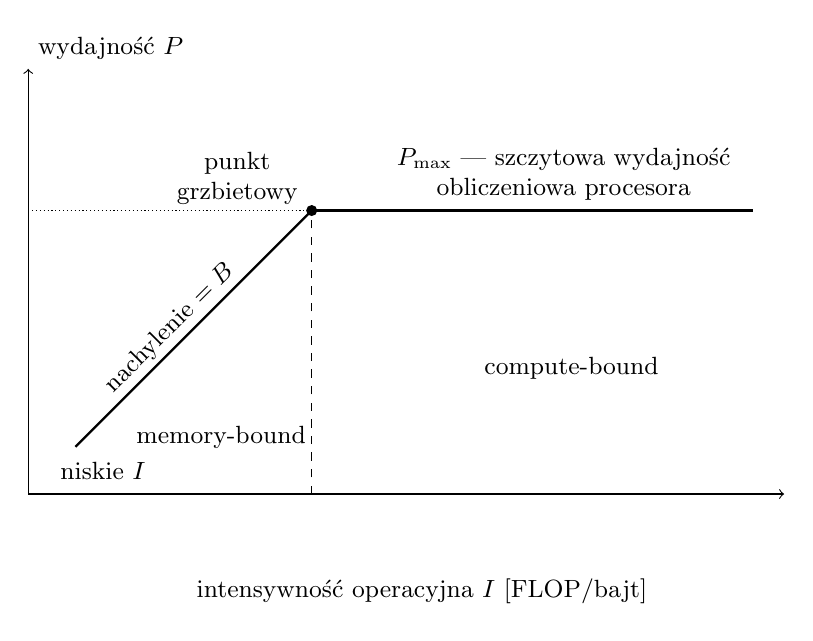
\begin{tikzpicture}[font=\small]
  \draw[->] (0,0) -- (9.6,0);
  \node[below] at (5.0,-0.95) {intensywność operacyjna $I$ [FLOP/bajt]};
  \draw[->] (0,0) -- (0,5.4) node[above right] {wydajność $P$};
  \draw[thick] (0.6,0.6) -- (3.6,3.6);
  \draw[thick] (3.6,3.6) -- (9.2,3.6);
  \draw[densely dotted] (0,3.6) -- (3.6,3.6);
  \node[above,align=center] at (6.8,3.6) {$P_{\max}$ --- szczytowa wydajność\\obliczeniowa procesora};
  \node[rotate=45,anchor=south,inner sep=2pt] at (1.95,1.95) {nachylenie $=B$};
  \fill (3.6,3.6) circle (2pt);
  \draw[dashed] (3.6,0) -- (3.6,3.6);
  \node[above left,align=center,inner sep=2pt] at (3.5,3.6) {punkt\\grzbietowy};
  \node at (0.95,0.3) {niskie $I$};
  \node at (2.45,0.72) {memory-bound};
  \node at (6.9,1.6) {compute-bound};
\end{tikzpicture}
\caption{Model roofline: osiągalna wydajność w funkcji intensywności operacyjnej. Pułap $P_{\max}$ wyznaczają liczba jednostek FMA, szerokość rejestrów wektorowych i częstotliwość procesora, a nachylenie skośnego pułapu --- przepustowość pamięci $B$. Operacje o niskim $I$ (np. iloczyn skalarny, mnożenie macierz--wektor) leżą na lewo od punktu grzbietowego}
\label{rys:roofline}
\end{figure}

Z tego powodu kluczem do wydajnych implementacji rozważanych w niniejszej pracy operacji jest świadome wykorzystanie pamięci podręcznej i lokalności danych. Pozostała część rozdziału opisuje budowę oraz organizację hierarchii pamięci i jednostek obliczeniowych konkretnego procesora docelowego, natomiast kolejny rozdział przedstawia techniki programistyczne pozwalające tę wiedzę wykorzystać.

\section{Pamięci półprzewodnikowe: SRAM i DRAM}
\label{sec:sram-dram}

Pamięć o dostępie swobodnym (ang. \emph{Random Access Memory}, RAM) występuje w dwóch odmianach: pamięci dynamicznej (ang. \emph{Dynamic RAM}, DRAM) oraz pamięci statycznej (ang. \emph{Static RAM}, SRAM) \cite{drepper2007memory}. Różnią się one budową komórki przechowującej pojedynczy bit, a wynikające z tego właściwości decydują o roli, jaką każda z nich pełni w hierarchii pamięci.

Komórka pamięci DRAM składa się z jednego tranzystora i jednego kondensatora (rysunek \ref{rys:dram-cell}). Bit zapisany jest jako obecność lub brak ładunku na kondensatorze, a tranzystor pełni funkcję przełącznika łączącego kondensator z linią danych, sterowanego linią adresową. Tak prosta budowa pozwala zmieścić ogromną liczbę komórek na małej powierzchni, co przekłada się na dużą pojemność i niski koszt w przeliczeniu na bit. Cena za to jest jednak wysoka: kondensator stopniowo traci ładunek wskutek prądów upływu, więc jego zawartość musi być cyklicznie odświeżana. Ponadto odczyt jest destrukcyjny (rozładowuje kondensator, który trzeba następnie naładować ponownie), a odczytany sygnał jest na tyle słaby, że wymaga wzmacniacza odczytu (ang. \emph{sense amplifier}). Operacje te wydłużają czas dostępu, dlatego DRAM stosuje się przede wszystkim jako pojemną pamięć operacyjną \cite{drepper2007memory}.

\begin{figure}[t!]
\centering
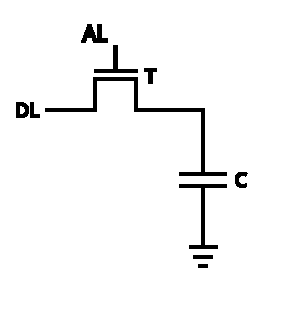
\includegraphics[width=0.3\textwidth]{DRAM_bit}
\caption{Komórka pamięci DRAM: jeden tranzystor i jeden kondensator}
\label{rys:dram-cell}
\end{figure}

Komórka pamięci SRAM jest znacznie bardziej rozbudowana: tworzy ją sześć tranzystorów (rysunek \ref{rys:sram-cell}). Cztery z nich są połączone w dwa sprzężone zwrotnie negatory, tworzące przerzutnik, który przechowuje bit, a dwa pozostałe pełnią rolę tranzystorów dostępowych. Tak zbudowana komórka utrzymuje zapisany stan w sposób stabilny tak długo, jak długo jest zasilana, bez potrzeby odświeżania --- stąd określenie ,,statyczna''. Odczyt nie narusza zawartości komórki, a sygnał wyjściowy jest silny i bliski cyfrowemu; w połączeniu z brakiem fazy odświeżania i aktywnym charakterem przerzutnika daje to bardzo krótki czas dostępu. Wadą jest zajmowana powierzchnia: sześć tranzystorów na bit oznacza znacznie mniejszą gęstość integracji i wyższy koszt niż w przypadku DRAM. Z tego powodu SRAM rezerwuje się dla niewielkich, lecz najszybszych poziomów hierarchii, przede wszystkim pamięci podręcznej \cite{drepper2007memory}.

\begin{figure}[t!]
\centering
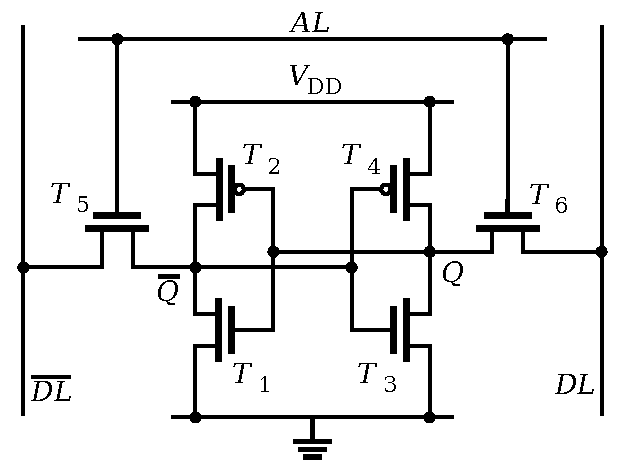
\includegraphics[width=0.5\textwidth]{SRAM_bit}
\caption{Komórka pamięci SRAM: sześć tranzystorów tworzących przerzutnik}
\label{rys:sram-cell}
\end{figure}

Zestawienie najważniejszych różnic przedstawia tabela \ref{tab:sram-dram}. Wynika z niego naturalny podział ról: szybka, lecz kosztowna SRAM buduje kolejne poziomy pamięci podręcznej, natomiast pojemna i tania DRAM pełni funkcję pamięci operacyjnej. Oba rodzaje pamięci współtworzą hierarchię, której organizację omówiono w kolejnym podrozdziale.

\begin{table}[t!]
\centering
\caption{Porównanie pamięci DRAM i SRAM}
\label{tab:sram-dram}
\begin{tabular}{lcc}
\hline
Cecha & DRAM & SRAM \\
\hline
Elementy na bit & 1 tranzystor + kondensator & 6 tranzystorów \\
Odświeżanie & wymagane & niewymagane \\
Czas dostępu & dłuższy & bardzo krótki \\
Gęstość integracji & duża & mała \\
Koszt na bit & niski & wysoki \\
Sygnał odczytu komórki & słaby, analogowy & silny, prawie cyfrowy \\
Typowe zastosowanie & pamięć operacyjna & pamięć podręczna \\
\hline
\end{tabular}
\end{table}

\section{Hierarchia pamięci podręcznej}
\label{sec:hierarchia}

Ponieważ żadna pojedyncza technologia nie łączy szybkości pamięci statycznej z pojemnością i niskim kosztem pamięci dynamicznej, współczesne procesory organizują pamięć w hierarchię złożoną z kilku poziomów (rysunek \ref{rys:hierarchia}). Im wyżej w hierarchii, tym pamięć jest szybsza, lecz mniejsza i droższa; im niżej --- wolniejsza, ale pojemniejsza i tańsza. Najwyższy poziom stanowią rejestry procesora, najniższy --- pamięć operacyjna, a poza nią pamięć masowa.

Pomiędzy rejestrami a pamięcią operacyjną umieszcza się pamięć podręczną (ang. \emph{cache}), niewielką, szybką pamięć zbudowaną z komórek SRAM, przechowującą kopie tych danych z pamięci głównej, do których spodziewany jest dostęp w najbliższym czasie \cite{drepper2007memory}. Współczesne procesory wyposaża się zwykle w trzy poziomy pamięci podręcznej, oznaczane L1, L2 oraz L3. Poziom L1 jest często rozdzielony na pamięć podręczną danych (L1D) i pamięć podręczną instrukcji (L1I). Poziomy L1 oraz L2 są prywatne dla każdego rdzenia, natomiast najpojemniejszy poziom L3 jest współdzielony przez rdzenie procesora \cite{evers2022zen3}.

Dane przemieszczają się między poziomami hierarchii w blokach o stałym rozmiarze, nazywanych liniami pamięci podręcznej (ang. \emph{cache line}). W procesorach budowanych w standardzie x86-64 linia liczy 64 bajty \cite{drepper2007memory}. Oznacza to, że nawet odwołanie do pojedynczego bajta powoduje sprowadzenie do pamięci podręcznej całej 64-bajtowej linii, co ma istotne konsekwencje dla efektywności dostępu do danych, omówione w rozdziale \ref{chap:lokalnosc}.

Gdy procesor żąda danej obecnej w pamięci podręcznej, następuje trafienie (ang. \emph{cache hit}) i dana zostaje dostarczona z niewielkim opóźnieniem. W przeciwnym razie zachodzi chybienie (ang. \emph{cache miss}): dana musi zostać sprowadzona z wolniejszego, niższego poziomu hierarchii, co znacznie wydłuża czas dostępu. Miarą uśrednionej wydajności hierarchii jest średni czas dostępu do pamięci (ang. \emph{average memory access time}, AMAT), który można wyrazić zależnością
\[
  t_{\mathrm{AMAT}} = t_{\mathrm{trafienia}} + p_{\mathrm{chybienia}} \cdot k_{\mathrm{chybienia}},
\]
gdzie $t_{\mathrm{trafienia}}$ oznacza czas dostępu przy trafieniu, $p_{\mathrm{chybienia}}$ --- prawdopodobieństwo chybienia, a $k_{\mathrm{chybienia}}$ --- dodatkowy koszt jego obsługi \cite{hennessy2017architecture}. Z zależności tej wynika, że hierarchia jest skuteczna tylko wtedy, gdy zdecydowana większość odwołań trafia do najszybszych poziomów, co umożliwia zasada lokalności omówiona w kolejnym rozdziale.

Pamięć podręczną charakteryzuje także jej drożność (ang. \emph{associativity}). Pamięć dzieli się na zbiory linii, a drożność określa, w ilu liniach danego zbioru może zostać umieszczony blok danych sprowadzany z pamięci głównej: w pamięci n-drożnej (ang. \emph{n-way}) każdy zbiór mieści $n$ linii. Większa drożność zmniejsza liczbę chybień wynikających z rywalizacji różnych adresów o to samo miejsce, lecz komplikuje i nieco spowalnia wyszukiwanie danej \cite{hennessy2017architecture}. Mechanizm odwzorowania adresów na zbiory i linie omówiono szczegółowo w kolejnym podrozdziale.

Konkretne parametry hierarchii dla procesora docelowego (AMD Ryzen 5 5600, mikroarchitektura Zen 3) przedstawia rysunek \ref{rys:hierarchia}. Pamięć podręczna L1 ma pojemność 32 KiB na dane oraz 32 KiB na instrukcje w każdym rdzeniu (8-drożna; opóźnienie ładowania od 4--5 cykli dla danych całkowitych do 7--8 cykli dla danych zmiennoprzecinkowych i wektorowych, a więc tych, na których operują jądra rozważane w pracy), L2 --- 512 KiB na rdzeń (8-drożna; opóźnienie zmienne, nie mniejsze niż 12 cykli), a współdzielona L3 --- 32 MiB (16-drożna; średnio około 46--47 cykli) \cite{amd_sog_19h,fog_microarchitecture}. Dostęp do pamięci operacyjnej, o pojemności wyrażanej w gigabajtach, wiąże się z opóźnieniem rzędu setek cykli.

Poziomy hierarchii w mikroarchitekturze Zen 3 różnią się również wzajemną relacją zawartości oraz przepustowością. Pamięć L2 jest inkluzywna względem L1, podczas gdy L3 pełni rolę pamięci ofiarnej (ang. \emph{victim cache}), wypełnianej liniami wypieranymi z L2, przez co jej zawartość w przybliżeniu nie powiela zawartości L2 \cite{amd_sog_19h}. O efektywnej pojemności szybkiej pamięci współdecyduje więc suma poziomów, co ma znaczenie przy doborze rozmiarów bloków (rozdział \ref{chap:lokalnosc}). Poziomy różni także przepustowość: z pamięci L1d można pobrać dwa 256-bitowe słowa na cykl, a ścieżka z L2 do L1 dostarcza 32 bajty na cykl \cite{amd_sog_19h,fog_microarchitecture}; konkretne wartości zestawiono w rozdziale poświęconym implementacji.

\begin{figure}[t!]
\centering
\begin{tikzpicture}[font=\small]
  \draw[fill=gray!8]  (1,0) rectangle (9,1);     \node at (5,0.5) {Pamięć operacyjna (DRAM)};
  \draw[fill=gray!12] (1.6,1) rectangle (8.4,2);  \node at (5,1.5) {Pamięć podręczna L3};
  \draw[fill=gray!16] (2.2,2) rectangle (7.8,3);  \node at (5,2.5) {Pamięć podręczna L2};
  \draw[fill=gray!20] (2.8,3) rectangle (7.2,4);  \node at (5,3.5) {Pamięć podręczna L1};
  \draw[fill=gray!24] (3.4,4) rectangle (6.6,5);  \node at (5,4.5) {Rejestry};
  \draw[dotted] (9,0.5) -- (9.3,0.5);   \node[right] at (9.3,0.5) {rzędu GB, setki cykli};
  \draw[dotted] (8.4,1.5) -- (9.3,1.5); \node[right] at (9.3,1.5) {32 MiB, $\approx$47 cykli};
  \draw[dotted] (7.8,2.5) -- (9.3,2.5); \node[right] at (9.3,2.5) {512 KiB, $\ge$12 cykli};
  \draw[dotted] (7.2,3.5) -- (9.3,3.5); \node[right] at (9.3,3.5) {32+32 KiB, 4--8 cykli};
  \draw[dotted] (6.6,4.5) -- (7.3,4.5); \node[right] at (7.3,4.5) {Operacje są wykonywane bezpośrednio tutaj};
  \draw[->] (0.6,0.2) -- (0.6,4.8);
  \node[rotate=90,anchor=south] at (0.35,2.5) {szybsza, mniejsza};
\end{tikzpicture}
\caption{Hierarchia pamięci w procesorze AMD Ryzen 5 5600 (Zen 3): od najszybszych rejestrów po pamięć operacyjną}
\label{rys:hierarchia}
\end{figure}

\section{Organizacja i adresowanie pamięci podręcznej}
\label{sec:organizacja}

Treść niniejszego podrozdziału opiera się głównie na pracach \cite{hennessy2017architecture} oraz \cite{gottlieb_arch_lec22}, w których zagadnienia te omówiono szczegółowo; w dalszej części odwołań tych nie powtarzamy.

Sposób, w jaki bloki danych z pamięci głównej są przypisywane do linii pamięci podręcznej, nazywamy odwzorowaniem. Wyróżnia się trzy podstawowe schematy. W odwzorowaniu bezpośrednim (ang. \emph{direct-mapped}) każdy blok może trafić do dokładnie jednej, z góry wyznaczonej linii (rozwiązanie proste i szybkie, lecz podatne na chybienia konfliktowe). W odwzorowaniu w pełni asocjacyjnym (ang. \emph{fully associative}) blok może zająć dowolną linię, co eliminuje konflikty, lecz wymaga porównania znacznika ze wszystkimi liniami i jest kosztowne sprzętowo. Kompromisem stosowanym w praktyce jest odwzorowanie zbiorowo-asocjacyjne (ang. \emph{set-associative}): pamięć dzieli się na zbiory, a blok przypisany jest do jednego zbioru, w obrębie którego może zająć dowolną z $n$ linii (pamięć $n$-drożna). Dwa pierwsze schematy są szczególnymi przypadkami trzeciego: odwzorowanie bezpośrednie odpowiada drożności równej 1, a odwzorowanie w pełni asocjacyjne --- drożności równej liczbie wszystkich linii pamięci podręcznej.

Aby odnaleźć daną w pamięci podręcznej, jej adres dzieli się na trzy pola, przedstawione na rysunku \ref{rys:adres}. Najmłodsze bity stanowią przesunięcie (OFFSET), wskazujące bajt w obrębie linii; ich liczba wynika z rozmiaru linii: dla linii 64-bajtowej jest to 6 bitów. Pole środkowe (SET) wskazuje zbiór, do którego należy blok, a jego szerokość zależy od liczby zbiorów. Najstarsze bity tworzą znacznik (TAG), który jednoznacznie identyfikuje blok przechowywany w linii.

\begin{figure}[t!]
\centering
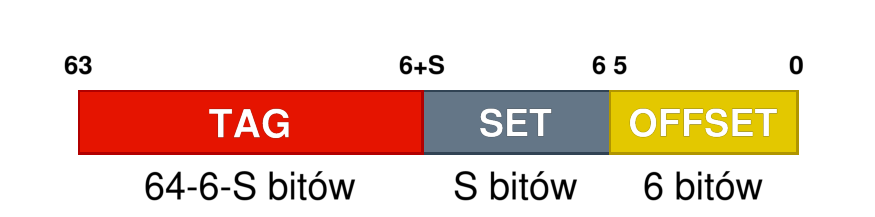
\includegraphics[width=0.85\textwidth]{cache_address}
\caption{Podział adresu na znacznik (TAG), numer zbioru (SET) i przesunięcie (OFFSET)}
\label{rys:adres}
\end{figure}

Wyszukiwanie danej przebiega następująco (rysunek \ref{rys:nway}): pole SET wybiera zbiór, po czym znacznik z adresu jest równolegle porównywany ze znacznikami wszystkich $n$ linii tego zbioru. Jeżeli któraś z linii ma zgodny znacznik oraz ustawiony bit ważności, następuje trafienie, a pole OFFSET wyłuskuje z jej zawartości żądany bajt; w przeciwnym razie zachodzi chybienie i blok musi zostać sprowadzony z niższego poziomu hierarchii.

\begin{figure}[t!]
\centering
\begin{tikzpicture}[font=\footnotesize]
  \node[above left] at (0,6.7) {Adres:};
  \draw (0,6) rectangle (3,6.7);   \node at (1.5,6.35) {znacznik (TAG)};
  \draw (3,6) rectangle (4.5,6.7); \node at (3.75,6.35) {SET};
  \draw (4.5,6) rectangle (6,6.7); \node at (5.25,6.35) {OFFSET};
  \node[draw, rounded corners, align=center, text width=6cm] (zbior) at (3,4.7) {zbiór wskazany przez pole SET\\($n$ linii, każda: znacznik i dane)};
  \node[draw, rounded corners, align=center, text width=6cm] (cmp) at (3,3.1) {równoległe porównanie znacznika z adresu ze znacznikami $n$ linii zbioru};
  \node[draw, rounded corners, align=center, text width=6cm] (hit) at (3,1.5) {trafienie $\Rightarrow$ pole OFFSET wskazuje żądany bajt w linii (dane)};
  \draw[->] (3.75,6) -- (3.75,5.25);
  \node[right,font=\scriptsize] at (3.9,5.6) {wybór zbioru};
  \draw[->] (zbior) -- (cmp);
  \draw[->] (cmp) -- (hit);
  \draw[->] (0,6.35) -- (-1.2,6.35) -- (-1.2,3.1) -- (cmp.west);
  \node[left,font=\scriptsize] at (-1.2,4.6) {znacznik};
  \draw[->] (6,6.35) -- (7.2,6.35) -- (7.2,1.5) -- (hit.east);
  \node[right,font=\scriptsize] at (7.2,4.0) {przesunięcie};
\end{tikzpicture}
\caption{Wyszukiwanie danej w pamięci podręcznej $n$-drożnej}
\label{rys:nway}
\end{figure}

Jeżeli przy chybieniu docelowy zbiór jest już zapełniony, jedna z jego linii musi zostać usunięta, aby zwolnić miejsce dla nowego bloku. O wyborze usuwanej linii decyduje polityka wymiany; najczęściej stosuje się zasadę najdawniej używanej linii (ang. \emph{least recently used}, LRU) bądź jej tańsze sprzętowo przybliżenia, a niekiedy wybór losowy.

Dla ilustracji rozważmy pamięć podręczną L1D procesora w architekturze Zen 3: pojemność 32 KiB, drożność 8, linia 64 B. Przesunięcie zajmuje 6 bitów, ponieważ linia liczy $64 = 2^{6}$ bajtów. Całkowita liczba linii wynosi $32768 / 64 = 512$, a przy ośmiu liniach w zbiorze daje to $512 / 8 = 64$ zbiory, zatem pole SET ma 6 bitów ($64 = 2^{6}$). Pozostałe, najstarsze bity adresu tworzą znacznik.

\section{Rejestry procesora}
\label{sec:rejestry}

Najwyższym i najszybszym poziomem hierarchii pamięci jest plik rejestrów procesora \cite{hennessy2017architecture}. Rejestry znajdują się bezpośrednio w rdzeniu, a jednostki wykonawcze odczytują z nich argumenty i zapisują do nich wyniki w czasie pojedynczego cyklu, bez konieczności sięgania do pamięci podręcznej. Dane przetwarzane przez procesor muszą zatem najpierw zostać załadowane z pamięci do rejestrów, a uzyskane wyniki --- zapisane z rejestrów z powrotem do pamięci.

Z punktu widzenia programu architektura x86-64 udostępnia szesnaście rejestrów architektonicznych ogólnego przeznaczenia o szerokości 64 bitów, którymi posługują się instrukcje do przechowywania liczb całkowitych oraz adresów \cite{amd64_apm_vol1}. Ich liczba jest niewielka i stała, dlatego efektywne wykorzystanie rejestrów stanowi istotny element optymalizacji: kompilator lub programista musi tak rozplanować obliczenia, aby możliwie długo utrzymywać często używane wartości w rejestrach i ograniczać kosztowne odwołania do pamięci. Sytuację, w której liczba jednocześnie potrzebnych wartości przekracza liczbę dostępnych rejestrów architektonicznych i wymusza tymczasowe odsyłanie ich do pamięci, określa się mianem presji rejestrowej (ang. \emph{register pressure}).

Fizyczna realizacja jest jednak bogatsza, niż sugeruje liczba rejestrów architektonicznych. Współczesne procesory wykonujące instrukcje poza kolejnością stosują przemianowywanie rejestrów (ang. \emph{register renaming}): szesnaście rejestrów architektonicznych jest dynamicznie odwzorowywanych na znacznie większy fizyczny plik rejestrów --- w mikroarchitekturze Zen 3 liczy on 192 rejestry całkowite \cite{fog_microarchitecture}. Mechanizm ten usuwa fałszywe zależności wynikające z ponownego użycia tej samej nazwy rejestru i umożliwia jednoczesne wykonywanie wielu instrukcji, co opisano dokładniej w kolejnym podrozdziale.

Oprócz rejestrów ogólnego przeznaczenia procesory x86-64 zawierają również rejestry wektorowe, umożliwiające równoległe przetwarzanie wielu wartości naraz. To one, wraz z odpowiadającymi im jednostkami wykonawczymi, są podstawą wektoryzacji obliczeń; ich budowę oraz wykorzystanie w rozszerzeniu AVX2 (ang. \emph{Advanced Vector Extensions 2}) omówiono w dalszej części niniejszego rozdziału.

\section{Droga dostępu do pamięci w rdzeniu procesora}
\label{sec:droga}

Odwołania do pamięci nie są kierowane do hierarchii pamięci wprost z instrukcji, lecz obsługują je wyspecjalizowane jednostki pobierające i zapisujące (ang. \emph{load/store units}). Adres każdego odwołania jest najpierw wyliczany, po czym żądanie trafia do kolejki, skąd kierowane jest do pamięci podręcznej L1. Mikroarchitektura Zen 3 potrafi wykonać do trzech operacji pamięciowych na cykl: do trzech odczytów albo do dwóch zapisów \cite{evers2022zen3}. Dla operacji na danych 256-bitowych (a takie wykonują jądra wektorowe rozważane w pracy) obowiązują ostrzejsze limity: najwyżej dwa odczyty oraz najwyżej jeden zapis 256-bitowy na cykl \cite{amd_sog_19h}.

Każde odwołanie posługuje się adresem wirtualnym, który przed dostępem do pamięci podręcznej musi zostać przetłumaczony na adres fizyczny. Tłumaczenie to przyspiesza bufor translacji adresów (ang. \emph{translation lookaside buffer}, TLB), niewielka pamięć podręczna przechowująca ostatnio używane odwzorowania stron. Podobnie jak dane, translacje organizuje się hierarchicznie: mikroarchitektura Zen 3 dysponuje osobnymi buforami TLB pierwszego i drugiego poziomu dla danych, obsługującymi strony o rozmiarach 4 KiB, 2 MiB oraz 1 GiB \cite{amd_sog_19h}. Chybienie w TLB wymusza kosztowne przejście tablic stron, dlatego wzorce dostępu rozrzucone po wielu stronach (na przykład kolumnowe przemiatanie dużej macierzy) mogą obniżać wydajność niezależnie od chybień w samej pamięci podręcznej danych; pakowanie omawiane w rozdziale \ref{chap:lokalnosc} ogranicza między innymi właśnie liczbę chybień TLB.

Współczesne rdzenie wykonują instrukcje poza kolejnością (ang. \emph{out-of-order execution}) \cite{hennessy2017architecture}. Po pobraniu i przemianowaniu rejestrów instrukcje trafiają do okna instrukcji, skąd są wydawane do wykonania, gdy tylko ich argumenty staną się dostępne --- niekoniecznie w kolejności wynikającej z programu. Aby zachować poprawność wyników, są one jednak zatwierdzane w pierwotnej kolejności za pomocą bufora zmiany kolejności (ang. \emph{reorder buffer}, ROB), który w mikroarchitekturze Zen 3 liczy 256 pozycji \cite{evers2022zen3}.

Najważniejszą konsekwencją wykonania poza kolejnością jest zdolność do obsługi wielu niezależnych odwołań do pamięci równocześnie, określana jako równoległość na poziomie pamięci (ang. \emph{memory-level parallelism}, MLP). Gdy jeden odczyt oczekuje na dane z wolniejszego poziomu hierarchii, procesor może wystawić kolejne, niezależne odczyty; ich opóźnienia wówczas się nakładają, zamiast sumować (rysunek \ref{rys:mlp}). W ten sposób znaczna część długiej latencji pamięci zostaje ukryta --- pod warunkiem jednak, że w programie istnieją niezależne odwołania, które można wykonać równolegle \cite{drepper2007memory}. Z tego względu regularny, przewidywalny wzorzec dostępu do danych ma kluczowe znaczenie dla wydajności; zagadnienie to rozwijamy w rozdziale \ref{chap:lokalnosc}.

\begin{figure}[t!]
\centering
\begin{tikzpicture}[font=\footnotesize]
  \node[left] at (-0.1,3.0) {bez MLP:};
  \draw[fill=gray!12] (0,2.7) rectangle (3,3.3); \node at (1.5,3.0) {odczyt A};
  \draw[fill=gray!12] (3,2.7) rectangle (6,3.3); \node at (4.5,3.0) {odczyt B};
  \draw[fill=gray!12] (6,2.7) rectangle (9,3.3); \node at (7.5,3.0) {odczyt C};
  \draw[<->] (0,3.7) -- (9,3.7); \node[above] at (4.5,3.7) {łączny czas oczekiwania};
  \node[left] at (-0.1,1.0) {z MLP:};
  \draw[fill=gray!12] (0,1.3) rectangle (3,1.7);    \node at (1.5,1.5) {odczyt A};
  \draw[fill=gray!12] (0.6,0.8) rectangle (3.6,1.2); \node at (2.1,1.0) {odczyt B};
  \draw[fill=gray!12] (1.2,0.3) rectangle (4.2,0.7); \node at (2.7,0.5) {odczyt C};
  \draw[<->] (0,2.05) -- (4.2,2.05); \node[above] at (2.1,2.05) {łączny czas oczekiwania};
  \draw[->] (0,-0.15) -- (9.8,-0.15) node[right] {czas};
  \draw[densely dashed] (9,-0.2) -- (9,3.6);
  \draw[densely dashed] (4.2,-0.2) -- (4.2,1.95);
\end{tikzpicture}
\caption{Równoległość na poziomie pamięci (MLP): nakładanie się opóźnień niezależnych odczytów skraca łączny czas oczekiwania}
\label{rys:mlp}
\end{figure}

\section{Jednostki wektorowe i FMA}
\label{sec:avx}

Obok skalarnych jednostek wykonawczych procesory x86-64 zawierają jednostki wektorowe, działające w modelu SIMD (ang. \emph{single instruction, multiple data}), jednej z klas w taksonomii Flynna \cite{flynn1972taxonomy}. W modelu tym pojedyncza instrukcja wykonuje tę samą operację na wielu danych jednocześnie. Rozszerzenie AVX wprowadziło rejestry wektorowe YMM o szerokości 256 bitów (w trybie 64-bitowym jest ich szesnaście), a AVX2 rozszerzyło zestaw operujących na nich instrukcji \cite{amd64_apm_vol1}. Pojedynczy rejestr YMM mieści cztery liczby zmiennoprzecinkowe podwójnej precyzji (po 64 bity) albo osiem liczb pojedynczej precyzji (rysunek \ref{rys:ymm}), które jednostka wektorowa przetwarza równolegle. Mikroarchitektura Zen 3 nie implementuje rozszerzenia AVX-512; najszerszymi rejestrami wektorowymi pozostają w niej 256-bitowe rejestry YMM, co przesądza o wyborze AVX2 jako docelowego zestawu instrukcji w implementacjach opisanych w dalszej części pracy.

Rozszerzenia AVX i AVX2 udostępniają między innymi wektorowe odczyty i zapisy (w wariancie wyrównanym oraz niewyrównanym do granicy 32 bajtów), operacje arytmetyczne na wektorach, a także instrukcje przestawiania i powielania danych w rejestrze; AVX2 dodało do nich m.in. 256-bitowe operacje całkowitoliczbowe oraz rozproszone odczyty (ang. \emph{gather}) \cite{gepner2017avx2}. Wyrównanie danych do granicy rejestru ma przy tym znaczenie dla wydajności odczytów wektorowych, do czego wracamy w rozdziale \ref{chap:lokalnosc}.

Szczególne znaczenie dla obliczeń numerycznych ma operacja złożonego mnożenia z dodawaniem (ang. \emph{fused multiply-add}, FMA), realizująca wyrażenie $a \cdot b + c$ w ramach jednej instrukcji i z pojedynczym zaokrągleniem wyniku \cite{ieee754_2008,zhang2019fma}. Stanowi ona podstawę wielu jąder obliczeniowych.

W mikroarchitekturze Zen 3 dostępne są dwie jednostki FMA, każda operująca na 256-bitowych rejestrach. Pojedyncza instrukcja FMA cechuje się opóźnieniem czterech cykli, lecz obie jednostki mogą przyjmować nową instrukcję w każdym cyklu \cite{fog_microarchitecture}. Aby w pełni wykorzystać potok, w wykonaniu musi znajdować się odpowiednio wiele niezależnych operacji --- co najmniej osiem, co wynika z przemnożenia liczby jednostek przez długość opóźnienia ($2 \times 4 = 8$). Dwie jednostki, z których każda przetwarza cztery wartości podwójnej precyzji oraz wykonuje mnożenie i dodawanie, dają przy taktowaniu około 4,4 GHz teoretyczną szczytową wydajność równą $2 \cdot 4 \cdot 2 \cdot 4{,}4 \approx 70$ miliardów operacji zmiennoprzecinkowych na sekundę --- jest to szczyt pojedynczego rdzenia przy maksymalnym taktowaniu przyspieszonym 4,4 GHz (taktowanie bazowe wynosi 3,5 GHz). Wydajność tę osiąga się jednak tylko wtedy, gdy dane docierają do jednostek odpowiednio szybko, co ponownie kieruje uwagę na hierarchię pamięci i lokalność danych.

\begin{figure}[t!]
\centering
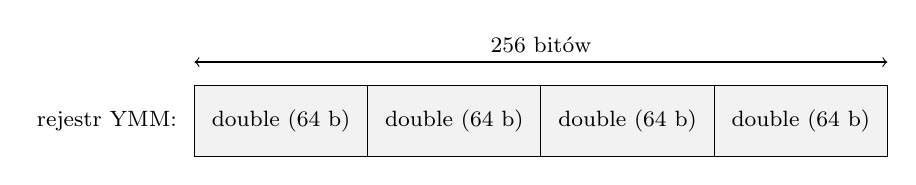
\begin{tikzpicture}[font=\footnotesize]
  \node[left] at (-0.1,0.45) {rejestr YMM:};
  \foreach \i in {0,1,2,3}{
    \draw[fill=gray!10] ({\i*2.2},0) rectangle ({\i*2.2+2.2},0.9);
    \node at ({\i*2.2+1.1},0.45) {double (64 b)};
  }
  \draw[<->] (0,1.2) -- (8.8,1.2);
  \node[above] at (4.4,1.2) {256 bitów};
\end{tikzpicture}
\caption{Rejestr wektorowy YMM (256 bitów) jako cztery liczby podwójnej precyzji; alternatywnie mieści osiem liczb pojedynczej precyzji}
\label{rys:ymm}
\end{figure}
\chapter{Lokalność danych i optymalizacja wykorzystania pamięci podręcznej}
\label{chap:lokalnosc}

\section{Zasada lokalności: czasowa i przestrzenna}
\label{sec:lokalnosc}

Skuteczność hierarchii pamięci opisanej w poprzednim rozdziale opiera się na spostrzeżeniu, że programy nie odwołują się do pamięci w sposób losowy, lecz w sposób wykazujący tak zwaną zasadę lokalności (ang. \emph{principle of locality}) \cite{hennessy2017architecture}. Wyróżnia się dwa jej rodzaje (lokalność czasową oraz przestrzenną), a hierarchia pamięci jest skonstruowana tak, aby obie wykorzystywać.

Lokalność czasowa (ang. \emph{temporal locality}) oznacza, że dana, do której nastąpiło odwołanie, prawdopodobnie zostanie wykorzystana ponownie w niedługim czasie. Hierarchia czerpie z niej korzyść, przechowując ostatnio używane dane w szybkich, leżących najwyżej warstwach, dzięki czemu kolejne odwołania do nich są tanie.

Lokalność przestrzenna (ang. \emph{spatial locality}) oznacza, że jeśli program odwołał się do pewnej komórki pamięci, to wkrótce prawdopodobnie odwoła się do komórek sąsiednich. Tę prawidłowość wykorzystuje się, sprowadzając dane całymi liniami pamięci podręcznej zamiast pojedynczymi bajtami (zob. podrozdział \ref{sec:hierarchia}); po sprowadzeniu jednej linii kolejne, sąsiadujące dane są już obecne w pamięci podręcznej \cite{drepper2007memory}.

Oba rodzaje lokalności ilustruje prosty przykład sumowania elementów tablicy (listing \ref{lst:lokalnosc}).

\begin{lstfloat}[t!]
\begin{lstlisting}[language=C, caption={Sumowanie elementów tablicy ilustrujące lokalność czasową i przestrzenną}, label={lst:lokalnosc}]
double suma = 0.0;
for (int i = 0; i < n; i++)
    suma += a[i];
\end{lstlisting}
\end{lstfloat}

W powyższej pętli zmienna \texttt{suma} jest odczytywana i zapisywana w każdej iteracji, wykazując lokalność czasową (w praktyce kompilator z włączonymi optymalizacjami utrzymuje ją w rejestrze, więc jej reużycie realizuje się na poziomie rejestrów; przykład ilustruje samą zasadę na poziomie wzorca odwołań). Tablica \texttt{a} jest natomiast przeglądana sekwencyjnie: kolejne elementy \texttt{a[i]} sąsiadują ze sobą w pamięci, więc po sprowadzeniu jednej linii pamięci podręcznej następnych kilka odwołań trafia już do niej --- to lokalność przestrzenna. Wzorce dostępu naruszające te zasady, takie jak duży krok lub dostęp w kolejności losowej, prowadzą do częstych chybień; sposoby ich unikania są przedmiotem dalszych podrozdziałów.

\section{Rodzaje chybień i wzorce dostępu}
\label{sec:chybienia}

Chybienia w pamięci podręcznej dzieli się tradycyjnie na trzy rodzaje, określane modelem 3C \cite{hill1989associativity,hennessy2017architecture}. Chybienia obowiązkowe (ang. \emph{compulsory}) zachodzą przy pierwszym odwołaniu do danego bloku, którego nie ma jeszcze w pamięci podręcznej. Chybienia pojemnościowe (ang. \emph{capacity}) wynikają z tego, że zbiór roboczy programu (ang. \emph{working set}), czyli zbiór danych używanych w danym okresie, przekracza pojemność pamięci podręcznej. Chybienia konfliktowe (ang. \emph{conflict}) pojawiają się natomiast wtedy, gdy zbyt wiele bloków odwzorowuje się na ten sam zbiór linii (przy ograniczonej drożności), mimo że pamięć jako całość nie jest zapełniona.

Liczba chybień silnie zależy od wzorca dostępu do danych. Dostęp sekwencyjny w pełni wykorzystuje lokalność przestrzenną. Dostęp ze stałym krokiem (ang. \emph{stride}) jest mniej efektywny --- jeśli krok przekracza rozmiar linii, każda sprowadzona linia dostarcza tylko jednego użytecznego elementu, a pozostała jej część zostaje zmarnowana (listing \ref{lst:stride}, rysunek \ref{rys:stride}).

\begin{lstfloat}[t!]
\begin{lstlisting}[language=C, caption={Dostęp do tablicy ze stałym krokiem: dla kroku równego jeden jest on sekwencyjny, dla większego --- z przeskokami}, label={lst:stride}]
double suma = 0.0;
for (int i = 0; i < n; i += krok)
    suma += a[i];
\end{lstlisting}
\end{lstfloat}

\begin{figure}[t!]
\centering
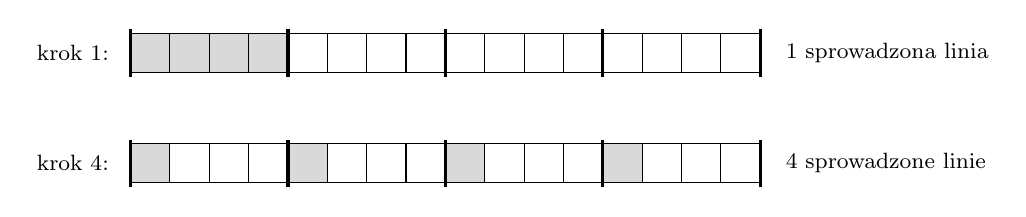
\begin{tikzpicture}[font=\footnotesize]
  \node[left] at (-0.15,2.25) {krok 1:};
  \foreach \i in {0,1,2,3}{ \fill[gray!30] (\i*0.5,2.0) rectangle (\i*0.5+0.5,2.5); }
  \foreach \i in {0,...,15}{ \draw (\i*0.5,2.0) rectangle (\i*0.5+0.5,2.5); }
  \foreach \l in {0,1,2,3,4}{ \draw[very thick] (\l*2,1.95) -- (\l*2,2.55); }
  \node[right] at (8.2,2.25) {1 sprowadzona linia};
  \node[left] at (-0.15,0.85) {krok 4:};
  \foreach \i in {0,4,8,12}{ \fill[gray!30] (\i*0.5,0.6) rectangle (\i*0.5+0.5,1.1); }
  \foreach \i in {0,...,15}{ \draw (\i*0.5,0.6) rectangle (\i*0.5+0.5,1.1); }
  \foreach \l in {0,1,2,3,4}{ \draw[very thick] (\l*2,0.55) -- (\l*2,1.15); }
  \node[right] at (8.2,0.85) {4 sprowadzone linie};
\end{tikzpicture}
\caption{Wpływ kroku dostępu na wykorzystanie linii pamięci podręcznej (dla uproszczenia linia mieści cztery elementy); szare pola oznaczają elementy, do których następuje odwołanie}
\label{rys:stride}
\end{figure}

Regularne wzorce dostępu są dodatkowo wspierane przez sprzętowy układ wstępnego pobierania danych (ang. \emph{hardware prefetcher}), który wykrywa sekwencyjne lub równomiernie krokowe strumienie odwołań i z wyprzedzeniem sprowadza kolejne linie, zanim procesor o nie poprosi \cite{drepper2007memory}. Dostęp nieregularny lub o losowej kolejności --- na przykład przeglądanie struktur powiązanych wskaźnikami --- pozbawia procesor tej korzyści i prowadzi do częstych chybień.

\section{Układ danych i transformacje pętli}
\label{sec:uklad}

O liczbie chybień decyduje nie tylko sam algorytm, lecz także rozmieszczenie danych w pamięci oraz kolejność, w jakiej program po nich przechodzi. Poniżej omówiono kilka technik poprawiających lokalność bez zmiany wyniku obliczeń \cite{drepper2007memory}.

Częstym wyborem projektowym jest sposób przechowywania danych złożonych. W układzie tablicy struktur (ang. \emph{array of structures}, AoS) pola jednego obiektu leżą w pamięci obok siebie, natomiast w układzie struktury tablic (ang. \emph{structure of arrays}, SoA) sąsiadują ze sobą te same pola kolejnych obiektów (listing \ref{lst:aossoa}). Gdy obliczenie korzysta tylko z jednego pola wielu obiektów, układ SoA zapewnia dostęp sekwencyjny i pełne wykorzystanie linii pamięci podręcznej, podczas gdy układ AoS przeplata w liniach pola nieużywane, marnując przepustowość (rysunek \ref{rys:aossoa}); układ SoA jest też znacznie łatwiejszy do zwektoryzowania \cite{intel_sdlt}.

\begin{lstfloat}[t!]
\begin{lstlisting}[language=C, caption={Dwa układy danych złożonych: tablica struktur (AoS) oraz struktura tablic (SoA)}, label={lst:aossoa}]
struct { double x, y, z; } aos[N];       /* AoS */
struct { double x[N], y[N], z[N]; } soa; /* SoA */
\end{lstlisting}
\end{lstfloat}

\begin{figure}[t!]
\centering
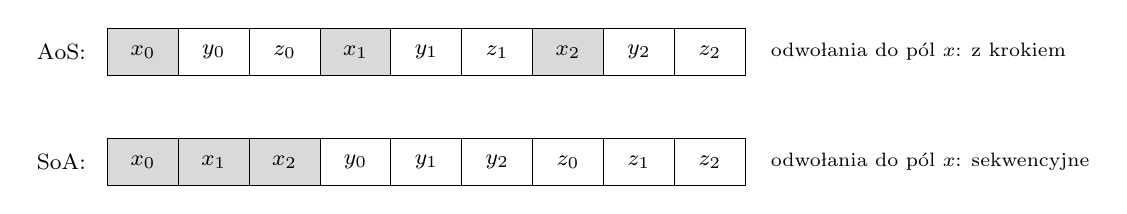
\begin{tikzpicture}[font=\footnotesize]
  \node[left] at (-0.15,1.8) {AoS:};
  \foreach \i in {0,3,6}{ \fill[gray!30] (\i*0.9,1.5) rectangle (\i*0.9+0.9,2.1); }
  \foreach \i in {0,...,8}{ \draw (\i*0.9,1.5) rectangle (\i*0.9+0.9,2.1); }
  \foreach \i/\lab in {0/{$x_0$},1/{$y_0$},2/{$z_0$},3/{$x_1$},4/{$y_1$},5/{$z_1$},6/{$x_2$},7/{$y_2$},8/{$z_2$}}{
    \node at (\i*0.9+0.45,1.8) {\lab};
  }
  \node[left] at (-0.15,0.4) {SoA:};
  \foreach \i in {0,1,2}{ \fill[gray!30] (\i*0.9,0.1) rectangle (\i*0.9+0.9,0.7); }
  \foreach \i in {0,...,8}{ \draw (\i*0.9,0.1) rectangle (\i*0.9+0.9,0.7); }
  \foreach \i/\lab in {0/{$x_0$},1/{$x_1$},2/{$x_2$},3/{$y_0$},4/{$y_1$},5/{$y_2$},6/{$z_0$},7/{$z_1$},8/{$z_2$}}{
    \node at (\i*0.9+0.45,0.4) {\lab};
  }
  \node[right,font=\scriptsize] at (8.3,1.8) {odwołania do pól $x$: z krokiem};
  \node[right,font=\scriptsize] at (8.3,0.4) {odwołania do pól $x$: sekwencyjne};
\end{tikzpicture}
\caption{Rozmieszczenie w pamięci obiektów o polach $x, y, z$: w układzie AoS sąsiadują pola jednego obiektu, w SoA --- te same pola kolejnych obiektów (szare pola oznaczają odwołania do pól $x$)}
\label{rys:aossoa}
\end{figure}

Na liczbę chybień konfliktowych wpływa również rozmieszczenie adresów danych: w szczególności odstęp między adresami kolejnych wierszy. Gdy długość wiersza tablicy jest potęgą dwójki, kolejne wiersze mogą odwzorowywać się na te same zbiory pamięci podręcznej, prowadząc do ich nadmiernej rywalizacji. Zapobiega temu dopełnienie (ang. \emph{padding}), czyli celowe rozszerzenie wiersza o kilka nieużywanych elementów, które rozsuwa adresy na różne zbiory. Dane przeznaczone do przetwarzania wektorowego dodatkowo wyrównuje się do granicy rejestru (32 bajtów w przypadku AVX2): wyrównany odczyt nigdy nie przecina granicy 64-bajtowej linii pamięci podręcznej, co eliminuje karę odczytu podzielonego, a ponadto umożliwia użycie wariantów instrukcji wymagających wyrównania.

Istotny jest wreszcie sam sposób przechodzenia po danych. Dostęp sekwencyjny po ciągłym obszarze pamięci sprzyja zarówno lokalności przestrzennej, jak i działaniu prefetchera. Jego przeciwieństwem jest ,,skakanie po wskaźnikach'' (ang. \emph{pointer chasing}) --- przechodzenie po strukturach takich jak listy czy drzewa, w których kolejne elementy leżą w nieprzewidywalnych miejscach pamięci. Taki wzorzec pozbawia procesor możliwości wstępnego pobierania i prowadzi do licznych chybień, dlatego dane intensywnie przetwarzane warto przechowywać w postaci ciągłych tablic.

Ostatnią z omawianych technik jest zamiana kolejności pętli (ang. \emph{loop interchange}) \cite{hennessy2017architecture}. W języku C tablice dwuwymiarowe przechowywane są wierszami (ang. \emph{row-major}): elementy jednego wiersza leżą w pamięci obok siebie. Pętla, której indeks wewnętrzny zmienia numer wiersza, odwołuje się więc do elementów odległych o całą długość wiersza --- z dużym krokiem --- podczas gdy zamiana pętli tak, by indeks wewnętrzny przebiegał kolumny jednego wiersza, daje dostęp sekwencyjny (rysunek \ref{rys:interchange}).

\begin{figure}[t!]
\centering
\begin{tikzpicture}[font=\footnotesize]
  \foreach \r in {0,1,2,3}{
    \foreach \c in {0,1,2,3}{
      \pgfmathtruncatemacro{\num}{\r*4+\c}
      \draw (\c,3-\r) rectangle (\c+1,4-\r);
      \node at (\c+0.5,3.5-\r) {\num};
    }
  }
  \draw[->,thick] (0.1,4.35) -- (3.9,4.35);
  \node[above,font=\scriptsize] at (2,4.4) {dostęp wierszami (sekwencyjny)};
  \draw[->,thick,dashed] (-0.4,3.9) -- (-0.4,0.1);
  \node[rotate=90,anchor=south,font=\scriptsize] at (-0.7,2) {dostęp kolumnami (z krokiem)};
\end{tikzpicture}
\caption{Macierz przechowywana wierszami (liczby oznaczają kolejność elementów w pamięci): dostęp wzdłuż wiersza jest sekwencyjny, a wzdłuż kolumny odbywa się z krokiem równym długości wiersza}
\label{rys:interchange}
\end{figure}

\section{Blokowanie i packing}
\label{sec:blokowanie}

Gdy zbiór roboczy obliczenia przekracza pojemność pamięci podręcznej, dane bywają wielokrotnie sprowadzane z wolniejszych poziomów, mimo że algorytm wykorzystuje je więcej niż raz. Rozwiązaniem jest blokowanie, nazywane też kafelkowaniem (ang. \emph{blocking}, tiling): podział przestrzeni obliczeń na małe kafelki, które mieszczą się w pamięci podręcznej i są w całości przetwarzane, zanim procesor przejdzie do następnego (rysunek \ref{rys:tiling}) \cite{drepper2007memory}. Dzięki temu dane sprowadzone do pamięci podręcznej są wykorzystywane wielokrotnie, zanim zostaną z niej wyparte.

\begin{figure}[t!]
\centering
\begin{tikzpicture}[font=\footnotesize]
  \fill[gray!30] (2.7,2.7) rectangle (4.05,4.05);
  \foreach \i in {0,...,9}{ \draw[gray!60] (\i*0.45,0) -- (\i*0.45,4.05); \draw[gray!60] (0,\i*0.45) -- (4.05,\i*0.45); }
  \foreach \i in {0,1,2,3}{ \draw[very thick] (\i*1.35,0) -- (\i*1.35,4.05); \draw[very thick] (0,\i*1.35) -- (4.05,\i*1.35); }
  \node[below] at (2.025,-0.2) {macierz};
  \draw[->] (5.9,3.4) -- (4.1,3.4);
  \node[right,align=left] at (5.9,3.4) {kafelek (mieści się\\w pamięci podręcznej)};
  \draw[->] (5.9,0.9) -- (3.85,0.25);
  \node[right] at (5.9,0.9) {pojedynczy element};
\end{tikzpicture}
\caption{Macierz dzielona na kafelki (grube linie), a każdy kafelek --- na pojedyncze elementy (cienkie linie); szary kafelek mieści się w pamięci podręcznej i jest przetwarzany w całości}
\label{rys:tiling}
\end{figure}

Blokowanie stosuje się zwykle na kilku poziomach naraz. Na najniższym poziomie, niewielki kafelek jest utrzymywany w rejestrach procesora, co maksymalizuje ponowne wykorzystanie załadowanych już wartości i minimalizuje liczbę odwołań do pamięci \cite{goto2008anatomy}. Na wyższych poziomach rozmiary kafelków dobiera się tak, aby mieściły się kolejno w pamięci podręcznej L1, L2 i L3; każdy poziom zapewnia, że dane sprowadzone do odpowiadającej mu warstwy są wielokrotnie wykorzystywane przed wyparciem (listing \ref{lst:blocking}).

\begin{lstfloat}[t!]
\begin{lstlisting}[language=C, caption={Szkic struktury pętli z blokowaniem: obliczenia wykonywane są kafelkami o boku $B$, mieszczącymi się w pamięci podręcznej. Zysk z blokowania pojawia się dopiero przy danych używanych wielokrotnie (jak w mnożeniu macierzy czy transpozycji), a nie przy pojedynczym przejściu pokazanym dla zwięzłości}, label={lst:blocking}]
for (int ii = 0; ii < n; ii += B)
    for (int jj = 0; jj < n; jj += B)
        for (int i = ii; i < ii + B; i++)
            for (int j = jj; j < jj + B; j++)
                /* przetwarzanie A[i][j] w kafelku B x B */
\end{lstlisting}
\end{lstfloat}

Samo blokowanie nie usuwa jednak problemu nieregularnego dostępu: kolejne wiersze kafelka wyciętego z dużej macierzy są w pamięci oddalone o całą długość wiersza, co prowadzi do dostępu z krokiem i chybień konfliktowych. Dlatego stosuje się pakowanie (ang. \emph{packing}), czyli skopiowanie kafelków do ciągłego, wyrównanego bufora, w którym układa się je jeden za drugim, w kolejności późniejszego przetwarzania. Dzięki temu program odczytuje dane w pełni sekwencyjnie, zarówno wewnątrz pojedynczego kafelka, jak i przy przechodzeniu między kolejnymi kafelkami, co praktycznie eliminuje chybienia konfliktowe wewnątrz spakowanego bufora i ogranicza liczbę dotykanych stron pamięci --- a więc i chybień w buforze translacji adresów (TLB) --- dobrze przy tym współgrając z prefetcherem \cite{goto2008anatomy}. Koszt tego kopiowania jest amortyzowany, ponieważ spakowane dane są następnie wykorzystywane wielokrotnie.
\section{Prefetching: sprzętowy i programowy}
\label{sec:prefetching}

Regularne wzorce dostępu są obsługiwane przez sprzętowe układy wstępnego pobierania (prefetchery), wspomniane już w podrozdziale \ref{sec:chybienia}. Mikroarchitektura Zen 3 wyposażona jest w kilka takich układów: prefetchery strumieniowe, sprowadzające kolejne sąsiednie linie; krokowe, rozpoznające stały krok między odwołaniami danej instrukcji; oraz regionowy, wykrywający powtarzalne wzorce w obrębie obszaru pamięci \cite{amd_sog_19h}. Z tego względu przewodnik optymalizacyjny AMD zaleca takie projektowanie struktur danych i wzorców dostępu, aby pasowały do działania tych prefetcherów; dane są wówczas sprowadzane z wyprzedzeniem, a długie latencje pamięci zostają ukryte.

Niezależnie od prefetcherów sprzętowych procesor udostępnia prefetch programowy, czyli jawną instrukcję (w języku C dostępną poprzez funkcję wbudowaną, listing \ref{lst:prefetch}), która z wyprzedzeniem nakazuje sprowadzenie wskazanej linii do pamięci podręcznej. Jest on użyteczny przede wszystkim tam, gdzie dostęp jest nieregularny, lecz przewidywalny z wyprzedzeniem --- na przykład przy przechodzeniu po strukturach powiązanych wskaźnikami, których prefetcher sprzętowy nie potrafi przewidzieć: znając wskaźnik do następnego elementu, można sprowadzić go, zanim stanie się potrzebny \cite{drepper2007memory}. Korzyść bywa jednak ograniczona, gdy przetwarzanie pojedynczego elementu jest krótkie --- wyprzedzenie o jeden węzeł daje wówczas zbyt mało czasu, by ukryć latencję sprowadzenia kolejnego \cite{drepper2007memory}.

\begin{lstfloat}[t!]
\begin{lstlisting}[language=C, caption={Prefetch programowy przy przechodzeniu listy: następny węzeł jest sprowadzany z wyprzedzeniem, podczas gdy przetwarzany jest bieżący}, label={lst:prefetch}]
while (p != NULL) {
    __builtin_prefetch(p->next);
    process(p);
    p = p->next;
}
\end{lstlisting}
\end{lstfloat}

Prefetch programowy stosuje się jednak z umiarem: sprowadzenie z wyprzedzeniem danych, które ostatecznie nie zostaną użyte, marnuje przepustowość pamięci i zapełnia pamięć podręczną niepotrzebnymi danymi \cite{drepper2007memory}. Dla regularnych, strumieniowych wzorców dostępu --- typowych dla rozważanych w pracy operacji --- prefetchery sprzętowe Zen 3 zwykle wystarczają, a jawny prefetch programowy rzadko przynosi dodatkowe korzyści, a bywa wręcz szkodliwy; polega się wówczas na prefetcherze sprzętowym \cite{lee2012prefetching,drepper2007memory}.

\section{Wektoryzacja jako technika dostępu i przepustowości}
\label{sec:wektoryzacja}

Wektoryzacja polega na wykorzystaniu jednostek wektorowych i FMA (podrozdział \ref{sec:avx}) do przetwarzania wielu danych jedną instrukcją. W języku C realizuje się ją najczęściej za pomocą funkcji wbudowanych (ang. \emph{intrinsics}), specjalnych funkcji odwzorowywanych bezpośrednio na instrukcje wektorowe procesora, dzięki którym programista jawnie steruje rejestrami oraz operacjami SIMD, nie sięgając po asembler \cite{gepner2017avx2}. Pojedynczy odczyt wektorowy sprowadza przy tym naraz kilka sąsiadujących w pamięci wartości, w pełni wykorzystując lokalność przestrzenną i całą linię pamięci podręcznej.

Aby odczyty wektorowe były wydajne, dane wyrównuje się do granicy rejestru (32 bajtów w AVX2), co pozwala wczytać wektor jedną, niepodzieloną operacją. Sama wektoryzacja przyspiesza jednak obliczenia tylko wtedy, gdy dane docierają do jednostek dostatecznie szybko; dlatego łączy się ją z omówionymi wcześniej technikami lokalności. Im więcej operacji wykonuje się na każdej załadowanej danej --- im wyższa intensywność operacyjna --- tym bardziej obliczenia przesuwają się w stronę ograniczenia mocą obliczeniową, a nie przepustowością pamięci \cite{williams2009roofline}.

Pełne wykorzystanie jednostek FMA wymaga ponadto utrzymywania w locie wielu niezależnych operacji --- na Zen 3 co najmniej ośmiu (podrozdział \ref{sec:avx}). Osiąga się to, prowadząc obliczenia w kilku niezależnych akumulatorach, których łańcuchy zależności nie blokują się nawzajem (listing \ref{lst:wektor}); w przedstawionym przykładzie rolę tę pełnią zmienne \texttt{acc0} oraz \texttt{acc1}.

\begin{lstfloat}[t!]
\begin{lstlisting}[language=C, caption={Zwektoryzowana pętla z funkcjami wbudowanymi AVX2: każda instrukcja FMA przetwarza cztery wartości double naraz, a dwa niezależne akumulatory częściowo ukrywają latencję potoku}, label={lst:wektor}]
__m256d acc0 = _mm256_setzero_pd();
__m256d acc1 = _mm256_setzero_pd();
for (int i = 0; i < n; i += 8) {
    acc0 = _mm256_fmadd_pd(_mm256_load_pd(a + i),     _mm256_load_pd(b + i),     acc0);
    acc1 = _mm256_fmadd_pd(_mm256_load_pd(a + i + 4), _mm256_load_pd(b + i + 4), acc1);
}
\end{lstlisting}
\end{lstfloat}

Przykład z dwoma akumulatorami ilustruje samą technikę prowadzenia wielu niezależnych łańcuchów obliczeń; dwa łańcuchy nie nasycają jednak w pełni obu jednostek FMA mikroarchitektury Zen 3, do czego potrzeba ośmiu niezależnych łańcuchów (podrozdział \ref{sec:avx}). Do tej liczby wraca rozdział poświęcony implementacji, w którym jądra obliczeniowe prowadzą obliczenia w odpowiednio większej liczbie akumulatorów.

\section{Równoległość a wykorzystanie pamięci podręcznej}
\label{sec:rownoleglosc}

Dotychczasowe rozważania dotyczyły pojedynczego rdzenia. Gdy obliczenia rozdziela się na wiele rdzeni, pojawiają się dodatkowe zjawiska związane z pamięcią podręczną. Równoległość rozważanych w pracy operacji zrealizowano za pomocą interfejsu OpenMP \cite{openmp52}, w którym pracę dzieli się między wątki, a każdy wątek przetwarza wydzieloną część danych.

Najniższe poziomy pamięci podręcznej (L1 i L2) są prywatne dla każdego rdzenia, natomiast poziom L3 jest współdzielony (podrozdział \ref{sec:hierarchia}). Rdzenie pracujące równolegle rywalizują więc o pojemność i przepustowość współdzielonej pamięci L3 oraz pamięci operacyjnej. Dla operacji ograniczonych przepustowością pamięci ma to istotną konsekwencję: ponieważ pułap przepustowości jest wspólny dla wszystkich rdzeni, dodawanie kolejnych wątków daje coraz mniejszy przyrost wydajności, w miarę jak łączne zapotrzebowanie na dane zbliża się do tego pułapu (powrót do modelu roofline z podrozdziału \ref{sec:motywacja}).

Szczególnie kosztownym zjawiskiem jest fałszywe współdzielenie (ang. \emph{false sharing}). Występuje ono, gdy dwa wątki działające na różnych rdzeniach modyfikują różne zmienne, które przypadkiem leżą w tej samej linii pamięci podręcznej (rysunek \ref{rys:falsesharing}). Każdy zapis dokonany przez jeden rdzeń unieważnia wówczas kopię linii w pamięci podręcznej drugiego rdzenia, zmuszając do jej ponownego sprowadzenia --- mimo że wątki nie współdzielą żadnych rzeczywistych danych. Przeciwdziała się temu, rozmieszczając dane przetwarzane przez różne wątki w osobnych liniach, na przykład przez wyrównanie lub dopełnienie struktur do rozmiaru linii \cite{drepper2007memory}.

\begin{figure}[t!]
\centering
\begin{tikzpicture}[font=\footnotesize]
  \node[font=\small] at (0.75,3.15) {Rdzeń 0};
  \node[font=\scriptsize] at (0.75,2.8) {zapisuje A};
  \fill[gray!25] (0,2) rectangle (0.75,2.6);
  \draw (0,2) rectangle (0.75,2.6); \node at (0.375,2.3) {A};
  \draw (0.75,2) rectangle (1.5,2.6); \node at (1.125,2.3) {B};
  \node[below,font=\scriptsize] at (0.75,2) {linia w cache rdzenia 0};
  \node[font=\small] at (7.25,3.15) {Rdzeń 1};
  \node[font=\scriptsize] at (7.25,2.8) {zapisuje B};
  \draw (6.5,2) rectangle (7.25,2.6); \node at (6.875,2.3) {A};
  \fill[gray!25] (7.25,2) rectangle (8,2.6);
  \draw (7.25,2) rectangle (8,2.6); \node at (7.625,2.3) {B};
  \node[below,font=\scriptsize] at (7.25,2) {linia w cache rdzenia 1};
  \draw[<->,thick] (1.6,2.3) -- (6.4,2.3);
  \node[above,align=center,font=\scriptsize] at (4,2.35) {ta sama linia wielokrotnie\\przesyłana między rdzeniami};
\end{tikzpicture}
\caption{Fałszywe współdzielenie: dwa rdzenie modyfikują różne zmienne (A oraz B) leżące w tej samej linii pamięci podręcznej, przez co linia jest wielokrotnie przesyłana między ich pamięciami podręcznymi mimo braku rzeczywistego współdzielenia danych}
\label{rys:falsesharing}
\end{figure}

Na koniec warto wspomnieć o niejednorodnym dostępie do pamięci (ang. \emph{non-uniform memory access}, NUMA), w którym czas dostępu do pamięci zależy od tego, który rdzeń żąda danych. W procesorze docelowym (Ryzen 5 5600) wszystkie rdzenie należą do jednego węzła pamięci, więc zjawisko to ma znaczenie marginalne; nabiera ono wagi dopiero w systemach wieloprocesorowych.

\section{Podejścia cache-aware i cache-oblivious}
\label{sec:aware-oblivious}

Algorytmy starające się efektywnie wykorzystać pamięć podręczną projektuje się według dwóch przeciwstawnych paradygmatów, różniących się stosunkiem do parametrów sprzętu.

W podejściu cache-aware (świadomym pamięci podręcznej) algorytm jawnie korzysta z rozmiarów pamięci podręcznej: parametry blokowania dobiera się tak, aby kafelki mieściły się w konkretnych poziomach hierarchii (jak w podrozdziale \ref{sec:blokowanie}) \cite{goto2008anatomy}. Zapewnia to wysoką wydajność na znanej maszynie, lecz wymaga dostrojenia parametrów do każdej platformy. W praktyce optymalne rozmiary kafelków często dobiera się empirycznie, metodą automatycznego strojenia (ang. \emph{auto-tuning}) --- stosowaną na przykład w bibliotece ATLAS \cite{whaley2001atlas} (podrozdział \ref{sec:blas-inne}): program mierzy wydajność dla różnych wartości parametrów i wybiera najlepsze dla danego procesora.

Przeciwnym podejściem jest cache-oblivious (nieświadome pamięci podręcznej), w którym algorytm (zwykle dzięki rekurencyjnemu podziałowi problemu na coraz mniejsze podproblemy) osiąga dobre wykorzystanie wszystkich poziomów hierarchii bez jawnej znajomości ich rozmiarów \cite{frigo1999cacheoblivious}. Jego zaletą jest przenośność, ponieważ ten sam kod działa efektywnie na różnych maszynach; wadą bywają większe stałe ukryte w złożoności oraz trudniejsza implementacja niż w starannie dostrojonym wariancie cache-aware.

Implementacje rozważanych w pracy operacji opierają się przede wszystkim na podejściu cache-aware --- z parametrami dobranymi do mikroarchitektury Zen 3. Szczegóły tych implementacji oraz uzyskane wyniki przedstawiono w kolejnych rozdziałach.

\chapter{BLAS: standard, implementacje i operacje}
\label{chap:blas}

\section{Czym jest BLAS --- geneza i rola}
\label{sec:blas-geneza}

BLAS (ang. \emph{Basic Linear Algebra Subprograms}) to ustalony zestaw podprogramów realizujących podstawowe operacje algebry liniowej, takie jak działania na wektorach oraz mnożenie macierzy przez wektor i macierzy przez macierz \cite{lawson1979blas}. Nie jest to konkretny program ani biblioteka, lecz specyfikacja interfejsu, czyli ściśle określony zbiór nazw procedur, list ich argumentów oraz wykonywanych przez nie operacji. Dzięki temu jedną i tę samą specyfikację może realizować wiele niezależnych implementacji, różniących się stopniem optymalizacji pod dany sprzęt.

Pomysł wydzielenia takiego zestawu wyrósł z dążenia do pogodzenia dwóch celów: przenośności oprogramowania numerycznego oraz jego wydajności \cite{lawson1979blas}. Algorytmy zawarte w BLAS (rozkłady macierzy, rozwiązywanie układów równań liniowych czy zagadnienia własne) w znacznej części czasu wykonują kilka powtarzalnych operacji elementarnych. Jeżeli operacje te ujmie się w wystandaryzowany interfejs, autor algorytmu wyższego poziomu może odwoływać się do nich za pośrednictwem ustalonych nazw, nie troszcząc się o szczegóły sprzętu. 

To rozdzielenie warstw stało się podstawą organizacji współczesnego oprogramowania numerycznego. Biblioteki wyższego poziomu, między innymi LAPACK (ang. \emph{Linear Algebra PACKage}), a za jej pośrednictwem liczne pakiety obliczeniowe, buduje się tak, aby najbardziej kosztowne obliczenia sprowadzały się do wywołań procedur BLAS \cite{blackford2002blas}. Ciężar optymalizacji przenosi się dzięki temu z wielu algorytmów na jedną, starannie dostrojoną warstwę podstawową.

Zestaw BLAS kształtował się stopniowo, w trzech etapach, którym odpowiada podział na trzy poziomy (ang. \emph{levels}). Poziom pierwszy (operacje wektor--wektor) zaproponowali w roku 1979 C. L. Lawson, R. J. Hanson, D. R. Kincaid i F. T. Krogh; obejmuje on takie działania jak iloczyn skalarny dwóch wektorów czy przeskalowanie wektora i dodanie go do innego (operacja postaci $y \leftarrow \alpha x + y$) \cite{lawson1979blas}. Poziom drugi (operacje macierz--wektor), wprowadzony w roku 1988 przez J. J. Dongarrę, J. Du Croza, S. Hammarlinga i R. J. Hansona, objął między innymi mnożenie macierzy przez wektor \cite{dongarra1988blas2}. Poziom trzeci (operacje macierz--macierz), opublikowany w roku 1990 przez J. J. Dongarrę, J. Du Croza, I. S. Duffa i S. Hammarlinga, dotyczy działań takich jak mnożenie dwóch macierzy \cite{dongarra1990blas3}. Kolejne poziomy odpowiadały rozwojowi architektur sprzętowych: poziom drugi opracowano przede wszystkim z myślą o procesorach wektorowych \cite{dongarra1988blas2}, a poziom trzeci --- o maszynach z hierarchią pamięci podręcznej \cite{dongarra1990blas3}. Znaczenie tego podziału dla wydajności jest przedmiotem następnego podrozdziału.

Z czasem BLAS stał się standardem przyjętym w środowisku obliczeń numerycznych: przyjęte konwencje nazw i list argumentów są wspólne dla wielu implementacji \cite{blackford2002blas}. Repozytorium Netlib udostępnia implementację referencyjną, napisaną w Fortranie, traktowaną jako wzorzec poprawności, a nie wydajności \cite{netlib_blas}. W roku 2002 grupa robocza BLAS Technical Forum opublikowała zaktualizowany i rozszerzony standard BLAS, kodyfikujący dotychczasowe konwencje i dodający nowe funkcjonalności: między innymi arytmetykę mieszanej i rozszerzonej precyzji oraz procedury dla macierzy rzadkich \cite{blackford2002blas}.

Pierwotną specyfikację BLAS sformułowano w języku Fortran \cite{blackford2002blas}, co odzwierciedlało dominację tego języka w obliczeniach naukowych w czasie powstawania zestawu. Aby udostępnić te same operacje programom pisanym w języku C, opracowano interfejs CBLAS (ang. \emph{C interface to the BLAS}) \cite{netlib_blas}. Zachowuje on funkcjonalność oryginału, dostosowując ją do konwencji języka C; istotną różnicą jest możliwość wskazania kolejności przechowywania elementów macierzy (wierszami lub kolumnami), podczas gdy interfejs Fortranu zakłada przechowywanie kolumnami.

Nazwy procedur BLAS podlegają zwartej konwencji: nazwa składa się z jednoliterowego przedrostka określającego typ danych oraz z rdzenia oznaczającego wykonywaną operację \cite{blackford2002blas}. Przedrostek przyjmuje jedną z czterech wartości zebranych w tabeli \ref{tab:blas-typy}. W poziomach drugim i trzecim rdzeń nazwy koduje dodatkowo strukturę macierzy: dwie litery bezpośrednio po przedrostku oznaczają jej typ (na przykład \texttt{ge} --- macierz ogólna, \texttt{sy} --- symetryczna, \texttt{tr} --- trójkątna), a dopiero pozostała część --- samą operację. I tak nazwę \texttt{dgemm} tworzą przedrostek \texttt{d} (podwójna precyzja), oznaczenie \texttt{ge} (macierz ogólna) oraz \texttt{mm} (mnożenie macierzy).

\begin{table}[t!]
\centering
\caption{Przedrostki nazw procedur BLAS określające typ danych}
\label{tab:blas-typy}
\begin{tabular}{cl}
\hline
Przedrostek & Typ danych \\
\hline
\texttt{s} & liczby rzeczywiste pojedynczej precyzji \\
\texttt{d} & liczby rzeczywiste podwójnej precyzji \\
\texttt{c} & liczby zespolone pojedynczej precyzji \\
\texttt{z} & liczby zespolone podwójnej precyzji \\
\hline
\end{tabular}
\end{table}

\section{Trzy poziomy BLAS i intensywność operacyjna}
\label{sec:blas-poziomy}

Podział zestawu BLAS na trzy poziomy ma znaczenie nie tylko historyczne i porządkujące, lecz przede wszystkim wydajnościowe. O tym, jak blisko szczytowej wydajności procesora można wykonać daną operację, decyduje bowiem nie sam rodzaj działania, lecz stosunek liczby wykonywanych operacji zmiennoprzecinkowych do ilości danych, które trzeba w tym celu przenieść między procesorem a pamięcią. Tu omawia się jego jakościowe konsekwencje dla trzech poziomów; dokładne wartości intensywności wyznaczono dla każdej z rozważanych operacji w podrozdziale \ref{sec:blas-operacje}, przyjmując liczby podwójnej precyzji, w których pojedynczy element zajmuje 8 bajtów.

Wielkością opisującą ten stosunek jest intensywność operacyjna $I$, wprowadzona w podrozdziale \ref{sec:motywacja}. Równoważnie, można posłużyć się klasyczną miarą $q$ --- liczbą działań przypadających na pojedyncze słowo (element) sprowadzone z wolniejszego poziomu pamięci \cite{williams2009roofline}:
\[
  q = \frac{f}{m},
\]
gdzie $f$ oznacza liczbę wykonanych działań, a $m$ --- liczbę słów przeniesionych między poziomami pamięci. Dla liczb podwójnej precyzji, zajmujących po 8 bajtów, obie miary wiąże zależność $I = q/8$. Im większa ich wartość, tym więcej obliczeń przypada na każdą sprowadzoną daną.

Trzy poziomy BLAS różnią się zasadniczo wartością intensywności operacyjnej, a wraz z nią --- charakterem wydajnościowym w świetle modelu roofline (podrozdział \ref{sec:motywacja}). Iloczyn skalarny i mnożenie macierzy przez wektor mają niską, w praktyce stałą intensywność, niezależną od rozmiaru zadania; leżą więc na lewo od punktu grzbietowego (rysunek \ref{rys:roofline}) i są ograniczone przepustowością pamięci (ang. \emph{memory-bound}): zwiększanie liczby jednostek arytmetycznych nie przyspieszy ich wykonania, skoro dane nie docierają dostatecznie szybko \cite{williams2009roofline}. Mnożenie macierzy, przeciwnie, ma intensywność rosnącą wraz z rozmiarem zadania i dla dostatecznie dużych rozmiarów przekracza punkt grzbietowy, stając się ograniczone mocą obliczeniową (ang. \emph{compute-bound}).

U podłoża tej różnicy leży zależność o charakterze geometrycznym, nazywana efektem powierzchnia--objętość (ang. \emph{surface-to-volume effect}). Liczba działań w mnożeniu macierzy rośnie jak iloczyn trzech wymiarów (dla macierzy kwadratowych --- jak $n^3$), a ilość przenoszonych danych --- jak suma iloczynów par wymiarów (jak $n^2$). Na poziomie trzecim pozostaje więc zapas pracy do wykonania na każdej sprowadzonej danej. Wykorzystują go blokowanie i pakowanie (podrozdział \ref{sec:blokowanie}): dzieląc macierze na kafelki mieszczące się w kolejnych poziomach pamięci podręcznej, podnoszą wartość $q$ aż do granicy wyznaczonej rozmiarem pamięci szybkiej. Granicę tę opisuje twierdzenie o złożoności wejścia--wyjścia: dla pamięci szybkiej o pojemności $M$ liczba słów przenoszonych między poziomami pamięci przy klasycznym mnożeniu macierzy wynosi co najmniej $\Omega\!\left(n^3/\sqrt{M}\right)$, czemu odpowiada intensywność $q = O\!\left(\sqrt{M}\right)$ \cite{hong1981redblue}. Ograniczenie to dotyczy klasycznego algorytmu sześciennego; algorytmy szybkiego mnożenia (podrozdział \ref{sec:blas-strassen}) podlegają innym, łagodniejszym oszacowaniom.

W rozważanych w pracy implementacjach optymalizuje się wszystkie trzy operacje, lecz cel i osiągalny pułap optymalizacji są odmienne. Techniki oparte na wielokrotnym wykorzystaniu danych (blokowanie i pakowanie) przynoszą zasadniczy zysk tam, gdzie ponowne użycie w ogóle występuje, czyli na poziomie trzecim, gdzie pozwalają zbliżyć się do szczytowej mocy obliczeniowej. Dla operacji ograniczonych przepustowością pamięci (poziom pierwszy i drugi) ponownych użyć niemal nie ma, więc optymalizacja (za pomocą wektoryzacji, wyrównania danych, uporządkowanego dostępu i prefetchingu) zmierza przede wszystkim do pełnego wykorzystania dostępnej przepustowości pamięci. Te różnice motywują dobór i sposób implementacji poszczególnych operacji w dalszej części pracy.

\section{Implementacje BLAS}
\label{sec:blas-implementacje}

Specyfikacja BLAS oddziela interfejs od sposobu jego realizacji, dzięki czemu tę samą operację może wykonywać wiele niezależnych implementacji, różniących się stopniem optymalizacji pod dany sprzęt (podrozdział \ref{sec:blas-geneza}). Poniżej omówiono implementacje istotne dla niniejszej pracy: referencyjną implementację z repozytorium Netlib oraz dwie biblioteki wysokiej wydajności (OpenBLAS i AOCL-BLAS), które w przeprowadzonych pomiarach służą jako punkt odniesienia. Krótko przedstawiono także kilka innych stosowanych implementacji BLAS.

\subsection{Implementacja referencyjna (Netlib)}
\label{sec:blas-netlib}

Repozytorium Netlib udostępnia referencyjną implementację BLAS, napisaną w języku Fortran 77 i obejmującą procedury wszystkich trzech poziomów we wszystkich czterech wariantach typu danych \cite{netlib_blas}. Pełni ona rolę wzorca poprawności, a nie wydajności: kod definiuje znaczenie poszczególnych operacji w sposób bezpośredni i przenośny, lecz bez jakiejkolwiek optymalizacji pod konkretną architekturę \cite{netlib_blas}. Operacje poziomu trzeciego (takie jak mnożenie macierzy) realizuje się w niej w postaci prostych, potrójnie zagnieżdżonych pętli, bez blokowania, pakowania czy jawnej wektoryzacji omówionych w rozdziale \ref{chap:lokalnosc}. W konsekwencji implementacja referencyjna nie jest zorganizowana pod kątem hierarchii pamięci podręcznej. Stanowi ona przez to naturalny punkt wyjścia --- definiuje oczekiwany wynik, względem którego weryfikuje się poprawność implementacji zoptymalizowanych.

\subsection{OpenBLAS}
\label{sec:blas-openblas}

OpenBLAS to otwarta biblioteka realizująca interfejs BLAS, wywodząca się z projektu GotoBLAS2 \cite{zhang2012openblas}. Jej pierwowzór, GotoBLAS, opracował Kazushige Goto w Texas Advanced Computing Center; biblioteka zasłynęła ręcznie pisanymi w asemblerze jądrami mnożenia macierzy, które przewyższały wydajnością kod generowany przez ówczesne kompilatory \cite{zhang2012openblas}. Po zakończeniu rozwoju GotoBLAS2 jego kod stał się podstawą OpenBLAS, rozwijanego jako otwarte oprogramowanie i utrzymywanego do dziś \cite{zhang2012openblas}.

Wysoką wydajność OpenBLAS osiąga dzięki ręcznie strojonym jądrom obliczeniowym, pisanym w asemblerze lub za pomocą funkcji wbudowanych (ang. \emph{intrinsics}), przygotowanym osobno dla wielu mikroarchitektur procesorów \cite{zhang2012openblas}. Wybór właściwego jądra dla procesora, na którym uruchomiono program, może następować w czasie wykonania: w trybie kompilacji obejmującym wiele architektur (opcja \texttt{DYNAMIC\_ARCH}) biblioteka rozpoznaje model procesora i dobiera odpowiedni wariant \cite{zhang2012openblas}. OpenBLAS udostępnia ponadto warianty wielowątkowe, w których pracę operacji dzieli się między rdzenie procesora.

\subsection{AOCL-BLAS}
\label{sec:blas-aocl}

AOCL-BLAS to implementacja BLAS rozwijana przez firmę AMD jako składnik pakietu AOCL (ang. \emph{AMD Optimizing CPU Libraries}), czyli zestawu bibliotek numerycznych zoptymalizowanych pod procesory oparte na architekturze ,,Zen'', w tym AMD Ryzen oraz EPYC \cite{amd_aocl_blas}. Biblioteka powstała jako rozwidlenie (ang. \emph{fork}) frameworka BLIS (ang. \emph{BLAS-like Library Instantiation Software}), opracowanego pierwotnie na University of Texas w Austin \cite{amd_aocl_blas,vanzee2015blis}. AMD utrzymuje swój wariant w synchronizacji z projektem macierzystym, dodając jądra i parametry blokowania dostrojone do kolejnych generacji rdzeni ,,Zen'' \cite{amd_aocl_blas}.

Architektura BLIS sprowadza całość obliczeń operacji poziomu drugiego i trzeciego do kilku bardzo prostych jąder \cite{vanzee2015blis}. Rdzeniem jest niewielkie, zależne od architektury mikrojądro (ang. \emph{micro-kernel}), realizujące mnożenie skrajnie małych bloków macierzy; otacza je przenośne makrojądro (ang. \emph{macro-kernel}), które dzieli pełną operację na podproblemy zgodnie z rozmiarami kafelków dobranymi do pamięci podręcznej \cite{vanzee2015blis}. Aby uzyskać implementację dla nowej architektury, wystarczy dostarczyć zoptymalizowane mikrojądro oraz dobrać parametry blokowania, podczas gdy przenośne makrojądro pozostaje niezmienione \cite{vanzee2015blis}.

\subsection{Inne implementacje BLAS}
\label{sec:blas-inne}

Poza implementacjami wykorzystanymi w pracy istnieje wiele innych realizacji interfejsu BLAS, różniących się platformą docelową, modelem licencyjnym oraz sposobem optymalizacji. Biblioteka Intel oneMKL (ang. \emph{oneAPI Math Kernel Library}, dawniej Intel Math Kernel Library) to zamknięta, własnościowa implementacja dostrojona pod procesory x86 firmy Intel, dostarczająca (obok BLAS) procedury LAPACK, transformaty Fouriera oraz inne funkcje obliczeniowe \cite{intel_onemkl}. Projekt ATLAS (ang. \emph{Automatically Tuned Linear Algebra Software}) reprezentuje odmienne podejście do optymalizacji: zamiast ręcznie pisanych jąder stosuje automatyczne strojenie empiryczne (podrozdział \ref{sec:aware-oblivious}), w którym podczas instalacji mierzy się wydajność wielu wariantów kodu i parametrów blokowania, a następnie wybiera najlepsze dla danej maszyny \cite{whaley2001atlas}. Biblioteka cuBLAS firmy NVIDIA realizuje z kolei interfejs BLAS na procesorach graficznych (GPU) w środowisku CUDA, kierując obliczenia na masywnie równoległą architekturę akceleratora zamiast na rdzenie procesora głównego \cite{nvidia_cublas}.

\section{Operacje implementowane w pracy}
\label{sec:blas-operacje}

Spośród operacji objętych specyfikacją BLAS w niniejszej pracy rozważa się trzy, po jednej z każdego poziomu: iloczyn skalarny (poziom pierwszy), mnożenie macierzy przez wektor (poziom drugi) oraz mnożenie dwóch macierzy (poziom trzeci). Poniżej przedstawiono ich definicje, podstawowe własności matematyczne oraz intensywność operacyjną; jej jakościowe konsekwencje dla trzech poziomów (ograniczenie przepustowością pamięci bądź mocą obliczeniową) omówiono w podrozdziale \ref{sec:blas-poziomy}.

\subsection{Iloczyn skalarny (poziom pierwszy)}
\label{sec:op-dot}

Iloczyn skalarny dwóch wektorów $\mathbf{x}$ i $\mathbf{y}$ o długości $N$ jest skalarem
\[
  s = \sum_{i=1}^{N} x_i\, y_i,
\]
a więc sumą iloczynów odpowiadających sobie składowych \cite{lawson1979blas,golub2013matrix}. Jest to najprostsza z rozważanych operacji, czyli działanie wektor--wektor należące do poziomu pierwszego BLAS, gdzie występuje pod nazwą \texttt{dot} (ang. \emph{dot product}) \cite{lawson1979blas}; wymaga $2N$ działań zmiennoprzecinkowych ($N$ mnożeń i $N$ dodawań).

Iloczyn skalarny jest także elementem składowym operacji wyższych poziomów: każda składowa wyniku mnożenia macierzy przez wektor w ujęciu wierszowym jest iloczynem skalarnym wiersza macierzy z wektorem, a każdy element iloczynu dwóch macierzy --- iloczynem skalarnym wiersza pierwszej macierzy z kolumną drugiej \cite{golub2013matrix}.

Pod względem wydajnościowym iloczyn skalarny reprezentuje najniższy poziom hierarchii BLAS. Wykonaniu $2N$ działań towarzyszy przeniesienie $(2N + 1)$ słów danych (obu wektorów wejściowych oraz zapisywanego wyniku skalarnego), czyli $(2N + 1)\times 8$ bajtów dla liczb podwójnej precyzji. Daje to intensywność operacyjną
\[
  I = \frac{2N}{8\,(2N + 1)} \approx \frac{1}{8} = 0{,}125 \text{ FLOP/bajt}
\]
($q \approx 1$). Wartość ta jest w praktyce stała --- nie rośnie wraz z długością wektorów, ponieważ każdy element bierze udział tylko w jednym mnożeniu i jednym dodawaniu. Iloczyn skalarny jest więc operacją silnie ograniczoną przepustowością pamięci (podrozdział \ref{sec:blas-poziomy}).

\subsection{Mnożenie macierzy przez wektor (poziom drugi)}
\label{sec:op-gemv}

Mnożenie macierzy przez wektor (ang. \emph{general matrix--vector multiply}, GEMV) jest operacją poziomu drugiego BLAS i realizuje przypisanie
\[
  \mathbf{y} \leftarrow \alpha A \mathbf{x} + \beta \mathbf{y},
\]
gdzie $A$ jest macierzą o wymiarach $M \times N$, $\mathbf{x}$ i $\mathbf{y}$ --- wektorami, a $\alpha$, $\beta$ --- skalarami \cite{dongarra1988blas2}.

Tę samą operację można zrealizować na dwa równoważne matematycznie sposoby, różniące się porządkiem dostępu do macierzy \cite{golub2013matrix}. W ujęciu wierszowym (ang. \emph{row-oriented}) każdą składową wektora wynikowego oblicza się niezależnie jako iloczyn skalarny odpowiedniego wiersza macierzy $A$ z wektorem $\mathbf{x}$:
\[
  y_i \leftarrow \beta\, y_i + \alpha \sum_{j=1}^{N} a_{ij}\, x_j .
\]
W ujęciu kolumnowym (ang. \emph{column-oriented}) cały wektor wynikowy aktualizuje się stopniowo, przebiegając kolumny macierzy $A$ i dodając każdą z nich do $\mathbf{y}$ z wagą równą odpowiedniej składowej $\mathbf{x}$:
\[
  \mathbf{y} \leftarrow \mathbf{y} + \alpha\, x_j\, A_{:,j}, \qquad j = 1, 2, \dots, N .
\]
Pojedynczy krok ujęcia kolumnowego jest operacją typu axpy (przeskalowanie wektora i dodanie go do innego, postaci $\mathbf{y} \leftarrow a\mathbf{x} + \mathbf{y}$), należącą (podobnie jak iloczyn skalarny) do poziomu pierwszego BLAS \cite{lawson1979blas,golub2013matrix}.

Pod względem wydajnościowym mnożenie macierzy przez wektor reprezentuje drugi poziom BLAS. Wykonaniu $2MN$ działań (po jednym mnożeniu i jednym dodawaniu na każdy z $MN$ elementów macierzy $A$) towarzyszy przeniesienie $(MN + N + 2M)\times 8$ bajtów, obejmujących macierz $A$, wektor wejściowy $\mathbf{x}$ oraz odczytywany i zapisywany wektor wynikowy $\mathbf{y}$. Daje to intensywność operacyjną
\[
  I = \frac{2MN}{8\,(MN + N + 2M)} \approx \frac{1}{4} = 0{,}25 \text{ FLOP/bajt}
\]
($q \approx 2$), gdyż dla dużych macierzy w bilansie danych dominuje człon $MN$. Również ta wartość pozostaje w praktyce stała, niezależnie od wymiarów macierzy: każdy element macierzy $A$ jest odczytywany tylko raz i bierze udział w jednym mnożeniu oraz jednym dodawaniu. Podobnie jak iloczyn skalarny, mnożenie macierzy przez wektor jest zatem operacją ograniczoną przepustowością pamięci (podrozdział \ref{sec:blas-poziomy}) \cite{williams2009roofline}.

\subsection{Mnożenie macierzy przez macierz (poziom trzeci)}
\label{sec:op-gemm}

Mnożenie dwóch macierzy (ang. \emph{general matrix multiply}, GEMM) jest operacją poziomu trzeciego BLAS i realizuje przypisanie
\[
  C \leftarrow \alpha A B + \beta C,
\]
gdzie $A$ ma wymiary $M \times K$, $B$ --- $K \times N$, $C$ --- $M \times N$, a $\alpha$, $\beta$ są skalarami \cite{dongarra1990blas3}. W klasycznym algorytmie każdy element macierzy wynikowej jest iloczynem skalarnym wiersza macierzy $A$ z kolumną macierzy $B$:
\[
  c_{ij} \leftarrow \beta\, c_{ij} + \alpha \sum_{k=1}^{K} a_{ik}\, b_{kj},
\]
co wymaga $2MNK$ działań zmiennoprzecinkowych \cite{golub2013matrix}. Mnożenie macierzy pełni rolę centralną w obliczeniach gęstej algebry liniowej: wiele algorytmów wyższego poziomu, w tym rozkłady macierzy realizowane w bibliotece LAPACK, sprowadza większość obliczeń do operacji poziomu trzeciego \cite{blackford2002blas,goto2008anatomy}, a pozostałe operacje tego poziomu można wyrazić za pomocą mnożenia macierzy \cite{kagstrom1998gemm}.

Pod względem wydajnościowym mnożenie macierzy wyróżnia się spośród rozważanych operacji. Wykonaniu $2MNK$ działań towarzyszy przeniesienie co najmniej $(MK + KN + 2MN)\times 8$ bajtów --- tyle wynosi minimalny, obowiązkowy ruch danych, w którym każdą z macierzy $A$, $B$ i $C$ przenosi się dokładnie raz; ruch rzeczywisty zależy od organizacji obliczeń. Daje to intensywność operacyjną
\[
  I = \frac{2MNK}{8\,(MK + KN + 2MN)}.
\]
Inaczej niż dla operacji niższych poziomów, intensywność ta nie jest ograniczona stałą: dla macierzy kwadratowych o boku $n$ przyjmuje wartość $n/16$ i rośnie wraz z rozmiarem macierzy, ponieważ każdy element bierze udział w wielu działaniach i po jednokrotnym sprowadzeniu z pamięci może zostać wielokrotnie wykorzystany. Dla dostatecznie dużych rozmiarów mnożenie macierzy jest więc operacją ograniczoną mocą obliczeniową (podrozdział \ref{sec:blas-poziomy}) \cite{williams2009roofline}. Liczbę działań, ilość przenoszonych danych oraz intensywność operacyjną wszystkich trzech rozważanych operacji zestawiono w tabeli \ref{tab:blas-intensywnosc}.

\begin{table}[t!]
\centering
\caption{Liczba działań, ilość przenoszonych danych i intensywność operacyjna dla operacji reprezentujących trzy poziomy BLAS (liczby podwójnej precyzji, $8$ bajtów na słowo; $N$ --- długość wektorów, $M$, $N$, $K$ --- wymiary macierzy; dla mnożenia dwóch macierzy wartości podano dla klasycznego algorytmu). Liczba słów danych oznacza minimalny, obowiązkowy ruch, w którym każdy operand przenosi się dokładnie raz}
\label{tab:blas-intensywnosc}
\begin{tabular}{clcccl}
\hline
Poziom & Operacja & Działania & Słowa danych & $I$ [FLOP/B] & Ograniczenie \\
\hline
1 & iloczyn skalarny & $2N$   & $2N+1$      & $\approx 0{,}125$ & pamięciowe \\
2 & macierz--wektor  & $2MN$  & $MN+N+2M$   & $\approx 0{,}25$  & pamięciowe \\
3 & macierz--macierz & $2MNK$ & $MK+KN+2MN$ & rośnie            & obliczeniowe \\
\hline
\end{tabular}
\end{table}

Klasyczny algorytm mnożenia macierzy wykonuje $2MNK$ działań, lecz nie jest pod tym względem optymalny: istnieją algorytmy szybkiego mnożenia, zmniejszające liczbę mnożeń kosztem większej liczby dodawań oraz gorszej stabilności numerycznej. Najbardziej znany z nich (algorytm Strassena) omówiono w następnym podrozdziale.

\section{Szybkie mnożenie macierzy: algorytm Strassena}
\label{sec:blas-strassen}

Klasyczny algorytm mnożenia dwóch macierzy o boku $n$ wykonuje liczbę działań proporcjonalną do $n^3$ --- ma więc złożoność sześcienną. Przez długi czas sądzono, że jest to granica nieprzekraczalna, gdyż każdy z $n^2$ elementów wyniku jest iloczynem skalarnym dwóch wektorów o długości $n$. Pogląd ten obalił w roku 1969 Volker Strassen, podając algorytm wykonujący asymptotycznie mniej działań niż metoda klasyczna \cite{strassen1969gaussian}. Niniejszy podrozdział przedstawia jego ideę oraz przyczyny, dla których wydajne biblioteki BLAS mimo to opierają się domyślnie na mnożeniu klasycznym.

Punktem wyjścia jest mnożenie dwóch macierzy o wymiarach $2 \times 2$. W ujęciu klasycznym wymaga ono $8$ mnożeń i $4$ dodawań elementów. Strassen zauważył, że ten sam iloczyn można obliczyć, używając jedynie siedmiu mnożeń, kosztem zwiększenia liczby dodawań i odejmowań \cite{strassen1969gaussian}. Spostrzeżenie to nabiera znaczenia, gdy potraktować elementy $2 \times 2$ nie jako liczby, lecz jako bloki (podmacierze): mnożenie bloków pozostaje mnożeniem macierzy, a dodawanie bloków jest tanie (koszt rzędu $n^2$), podczas gdy mnożenie jest kosztowne (koszt rzędu $n^3$). Zamiana jednego mnożenia bloków na kilka dodawań opłaca się więc tym bardziej, im większe są bloki.

Niech mnożone macierze $A$ i $B$ oraz wynik $C = AB$ będą podzielone na cztery bloki o boku $n/2$:
\[
  A = \begin{bmatrix} A_{11} & A_{12} \\ A_{21} & A_{22} \end{bmatrix}, \qquad
  B = \begin{bmatrix} B_{11} & B_{12} \\ B_{21} & B_{22} \end{bmatrix}, \qquad
  C = \begin{bmatrix} C_{11} & C_{12} \\ C_{21} & C_{22} \end{bmatrix}.
\]
Algorytm Strassena oblicza najpierw siedem iloczynów pośrednich $M_1, \dots, M_7$, z których każdy jest pojedynczym mnożeniem bloków:
\[
  \begin{aligned}
    M_1 &= (A_{11} + A_{22})(B_{11} + B_{22}), &\qquad M_2 &= (A_{21} + A_{22})\,B_{11}, \\
    M_3 &= A_{11}\,(B_{12} - B_{22}),           &\qquad M_4 &= A_{22}\,(B_{21} - B_{11}), \\
    M_5 &= (A_{11} + A_{12})\,B_{22},           &\qquad M_6 &= (A_{21} - A_{11})(B_{11} + B_{12}), \\
    M_7 &= (A_{12} - A_{22})(B_{21} + B_{22}). &&
  \end{aligned}
\]
Bloki macierzy wynikowej odtwarza się następnie wyłącznie przez dodawanie i odejmowanie iloczynów pośrednich \cite{strassen1969gaussian}:
\[
  \begin{aligned}
    C_{11} &= M_1 + M_4 - M_5 + M_7, &\qquad C_{12} &= M_3 + M_5, \\
    C_{21} &= M_2 + M_4,             &\qquad C_{22} &= M_1 - M_2 + M_3 + M_6.
  \end{aligned}
\]
Łącznie schemat ten wykorzystuje siedem mnożeń bloków oraz osiemnaście dodawań i odejmowań bloków --- wobec ośmiu mnożeń i czterech dodawań w metodzie klasycznej. Podział macierzy $A$, $B$ i $C$ na bloki przedstawia rysunek \ref{rys:strassen}.

Sama redukcja jednego mnożenia w pojedynczym kroku nie dawałaby zysku --- przeciwnie, dodatkowe dodawania zwiększyłyby koszt. Istota algorytmu tkwi w jego rekurencyjnym zastosowaniu: każde z siedmiu mnożeń bloków $(n/2) \times (n/2)$ wykonuje się tym samym schematem Strassena, dzieląc bloki na jeszcze mniejsze, i tak dalej \cite{strassen1969gaussian}. Liczba mnożeń skalarnych spełnia wówczas zależność rekurencyjną $T(n) = 7\,T(n/2)$, której rozwiązaniem jest $T(n) = \Theta\!\left(n^{\log_2 7}\right)$. Dodawania bloków wnoszą na każdym poziomie rekursji koszt rzędu $\Theta(n^2)$, więc pełna liczba działań spełnia rekurencję $T(n) = 7\,T(n/2) + \Theta(n^2)$, której rozwiązaniem --- na mocy twierdzenia o rekurencji uniwersalnej --- również jest $\Theta\!\left(n^{\log_2 7}\right)$, gdyż dominuje w niej człon rekurencyjny. Ponieważ $\log_2 7 \approx 2{,}807$, algorytm Strassena ma złożoność $O\!\left(n^{2{,}807}\right)$, asymptotycznie niższą niż $O\!\left(n^3\right)$ metody klasycznej \cite{strassen1969gaussian,higham1990exploiting}. Rekurencyjny podział na siedem podproblemów o połowie rozmiaru --- przeciwstawiony ośmiu podproblemom mnożenia klasycznego --- jest źródłem asymptotycznej przewagi algorytmu.

\begin{figure}[t!]
\centering
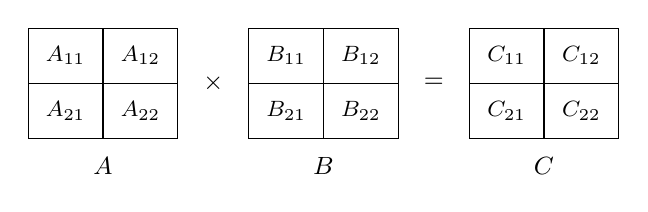
\begin{tikzpicture}[
  font=\footnotesize,
  blk/.style={draw, minimum width=0.95cm, minimum height=0.7cm, inner sep=0},
  opis/.style={font=\small},
]
% Macierz A
\begin{scope}[xshift=0cm]
  \node[blk] at (-0.475, 0.35) {$A_{11}$};
  \node[blk] at ( 0.475, 0.35) {$A_{12}$};
  \node[blk] at (-0.475,-0.35) {$A_{21}$};
  \node[blk] at ( 0.475,-0.35) {$A_{22}$};
  \node[opis] at (0,-1.05) {$A$};
\end{scope}
\node[opis] at (1.4,0) {$\times$};
% Macierz B
\begin{scope}[xshift=2.8cm]
  \node[blk] at (-0.475, 0.35) {$B_{11}$};
  \node[blk] at ( 0.475, 0.35) {$B_{12}$};
  \node[blk] at (-0.475,-0.35) {$B_{21}$};
  \node[blk] at ( 0.475,-0.35) {$B_{22}$};
  \node[opis] at (0,-1.05) {$B$};
\end{scope}
\node[opis] at (4.2,0) {$=$};
% Macierz C
\begin{scope}[xshift=5.6cm]
  \node[blk] at (-0.475, 0.35) {$C_{11}$};
  \node[blk] at ( 0.475, 0.35) {$C_{12}$};
  \node[blk] at (-0.475,-0.35) {$C_{21}$};
  \node[blk] at ( 0.475,-0.35) {$C_{22}$};
  \node[opis] at (0,-1.05) {$C$};
\end{scope}
\end{tikzpicture}
\caption{Podział macierzy $A$, $B$ i $C$ na bloki o boku $n/2$ w algorytmie Strassena. Cztery bloki macierzy wynikowej $C_{11}, C_{12}, C_{21}, C_{22}$ oblicza się z siedmiu iloczynów pośrednich $M_1, \dots, M_7$ (zamiast ośmiu w metodzie klasycznej), według wzorów podanych w tekście.}
\label{rys:strassen}
\end{figure}

W praktyce rekurencji nie prowadzi się aż do bloków pojedynczych elementów. Poniżej pewnego rozmiaru bloku, zwanego progiem odcięcia (ang. \emph{crossover}), zaprzestaje się podziału i mnoży bloki klasycznym, lecz zoptymalizowanym jądrem \cite{higham1990exploiting}. Przyczyna jest dwojaka. Po pierwsze, dla małych macierzy narzut osiemnastu dodawań bloków oraz tworzenia macierzy pośrednich przeważa nad oszczędnością wynikającą z jednego mniejszego mnożenia, więc próg opłacalności względem dobrego jądra klasycznego sięga rozmiarów rzędu co najmniej stu wierszy i kolumn, a wobec najlepiej zoptymalizowanych jąder bibliotecznych --- typowo kilkuset \cite{higham1990exploiting}. Po drugie, to właśnie klasyczne mnożenie małych bloków --- a nie rekurencja Strassena --- pozwala w pełni wykorzystać pamięć podręczną i rejestry, stosując blokowanie oraz packing opisane w podrozdziale \ref{sec:blokowanie}. Sam rekurencyjny podział macierzy na coraz mniejsze bloki ma przy tym charakter zbliżony do strategii cache-oblivious (podrozdział \ref{sec:aware-oblivious}): zmniejszając podproblem, wcześniej czy później sprowadza go do rozmiaru mieszczącego się w pamięci szybkiej, niezależnie od jej konkretnej pojemności \cite{frigo1999cacheoblivious}.

Schemat Strassena doczekał się wariantu o mniejszej liczbie dodawań, opracowanego przez Winograda i nazywanego algorytmem Strassena--Winograda. Zachowuje on siedem mnożeń bloków, lecz dzięki ponownemu wykorzystaniu wspólnych sum pośrednich ogranicza liczbę dodawań i odejmowań bloków z osiemnastu do piętnastu, co zmniejsza narzut dla danego rozmiaru bloku \cite{higham1990exploiting}. Asymptotyczna złożoność pozostaje przy tym taka sama, $O\!\left(n^{\log_2 7}\right)$.

Algorytm Strassena nie jest kresem teoretycznych możliwości. Najmniejszy wykładnik $\omega$, przy którym istnieje algorytm mnożenia macierzy o złożoności $O\!\left(n^{\omega}\right)$, jest przedmiotem trwających badań: w roku 1990 Coppersmith i Winograd obniżyli go do $\omega \approx 2{,}376$ \cite{coppersmith1990matrix}. Kolejne udoskonalenia tej metody obniżały ograniczenie dalej --- do $\omega < 2{,}3729$ (Alman i Williams, 2021) \cite{alman2021refined}, a w najnowszych pracach do $\omega < 2{,}3716$ (Williams, Xu, Xu i Zhou, 2024) \cite{williams2024omega} oraz $\omega < 2{,}3714$ (Alman i in., 2025) \cite{alman2025omega}. Algorytmy osiągające te wykładniki mają jednak wyłącznie znaczenie teoretyczne --- są to tak zwane algorytmy galaktyczne (ang. \emph{galactic algorithms}, termin wprowadzili R. J. Lipton i K. W. Regan): ukryte w notacji asymptotycznej stałe są tak ogromne, że przewaga nad metodami klasycznymi ujawniłaby się dopiero dla macierzy o rozmiarach przekraczających jakiekolwiek praktyczne zastosowania \cite{alman2021refined}.

Mimo asymptotycznej przewagi szybkie mnożenie macierzy wiąże się z kompromisami, które ograniczają jego zastosowanie w bibliotekach BLAS. Po pierwsze, jest ono gorsze numerycznie od mnożenia klasycznego: oszacowania błędu zaokrągleń są dla niego słabsze i mają charakter normowy, a nie składnikowy, a dokładność pogarsza się wraz z głębokością rekurencji \cite{higham1990exploiting}. Dla wielu zastosowań pozostaje ono jednak dostatecznie dokładne \cite{higham1990exploiting}. Po drugie, schemat Strassena potrzebuje dodatkowej pamięci roboczej na iloczyny pośrednie $M_1, \dots, M_7$ oraz sumy bloków, a jej objętość rośnie wraz z rozmiarem macierzy; klasycznemu mnożeniu blokowanemu wystarczają natomiast niewielkie bufory pakowania o stałym rozmiarze. Po trzecie, przewaga ujawnia się dopiero dla dużych macierzy, powyżej progu odcięcia. Z tych powodów wydajne implementacje BLAS --- w tym omawiane w podrozdziale \ref{sec:blas-implementacje} --- realizują mnożenie macierzy domyślnie metodą klasyczną, opartą na blokowaniu i packingu (podrozdział \ref{sec:blokowanie}), traktując algorytm Strassena co najwyżej jako technikę uzupełniającą dla bardzo dużych macierzy \cite{higham1990exploiting,goto2008anatomy}.

\chapter{Operacja splotu i metody jej obliczania}
\label{chap:splot}

\section{Czym jest splot --- definicja i zastosowania}
\label{sec:splot-definicja}

Splot (ang. \emph{convolution}) jest operacją dwuargumentową, która z dwóch funkcji tworzy trzecią, opisującą, jak kształt jednej z nich jest modyfikowany przez drugą. W zastosowaniach numerycznych pracuje się z postacią dyskretną tej operacji, w której argumenty są ciągami wartości spróbkowanych w równych odstępach \cite{oppenheim2010dtsp}. Dla dwóch ciągów jednowymiarowych $x$ oraz $w$, określonych dla całkowitych indeksów, splot dyskretny definiuje się jako
\[
  (x * w)[t] = \sum_{a=-\infty}^{\infty} x[a]\, w[t - a],
\]
a więc jako sumę iloczynów wartości pierwszego ciągu i przesuniętych, odbitych wartości drugiego \cite{oppenheim2010dtsp,goodfellow2016deeplearning}. W terminologii sieci splotowych pierwszy argument $x$ nazywa się wejściem (ang. \emph{input}), drugi --- $w$ --- jądrem (ang. \emph{kernel}), a wynik operacji --- mapą cech (ang. \emph{feature map}) \cite{goodfellow2016deeplearning}. W praktyce jądro ma skończony, niewielki nośnik, więc nieskończone sumowanie sprowadza się do sumy po kilku składnikach.

Operację rozszerza się na dwa wymiary, gdy wejściem jest obraz $I$, a jądrem dwuwymiarowa tablica $K$. Splot dwuwymiarowy przyjmuje wówczas postać \cite{goodfellow2016deeplearning}
\[
  S[i, j] = (I * K)[i, j] = \sum_{m} \sum_{n} I[m, n]\, K[i - m, j - n].
\]
Splot jest przemienny: równoważnie można zapisać $S[i, j] = \sum_{m} \sum_{n} I[i - m, j - n]\, K[m, n]$, gdzie zamieniono role argumentów \cite{goodfellow2016deeplearning}. Przemienność ta wynika wprost z odbicia jądra względem wejścia: wraz ze wzrostem indeksu sumowania indeks wejścia rośnie, a indeks jądra maleje \cite{goodfellow2016deeplearning}.

Od splotu należy odróżnić blisko z nim spokrewnioną korelację krzyżową (ang. \emph{cross-correlation}), która jest tą samą operacją, lecz bez odbicia jądra \cite{goodfellow2016deeplearning,oppenheim2010dtsp}:
\[
  S[i, j] = \sum_{m} \sum_{n} I[i + m, j + n]\, K[m, n].
\]
Różnica sprowadza się więc do znaku przy indeksach jądra: w splocie jądro jest odbite, w korelacji krzyżowej --- nie. Dla jąder symetrycznych względem środka (przechodzących na siebie przy obrocie o $180^\circ$) obie operacje dają identyczny wynik. Rozróżnienie to ma znaczenie w opisie, ponieważ to, co w uczeniu głębokim powszechnie nazywa się ,,splotem'', jest w istocie korelacją krzyżową: wiele bibliotek uczenia maszynowego implementuje korelację krzyżową, lecz określa ją mianem splotu \cite{goodfellow2016deeplearning}. Odbicie jądra jest tam zbędne, gdyż wagi jądra i tak są wyznaczane w procesie uczenia. W niniejszej pracy przyjęto natomiast definicję ścisłą: implementowane jądra obliczają splot właściwy, z jądrem odbitym w obu wymiarach przestrzennych. Wybór ten nie zmienia charakteru obliczeniowego operacji (liczba działań i wzorzec dostępu do wejścia pozostają takie same, a odbicie sprowadza się do odwróconej kolejności odczytu wag), więc wszystkie omawiane dalej techniki optymalizacji stosują się jednakowo do obu wariantów.

W sieciach splotowych operacja występuje w postaci wielokanałowej. Wejściem jest wówczas tensor o $C_{\mathrm{in}}$ kanałach i wymiarach przestrzennych $H \times W$, a zbiorem jąder --- tensor czterowymiarowy o wymiarach $C_{\mathrm{out}} \times C_{\mathrm{in}} \times K_H \times K_W$, opisujący $C_{\mathrm{out}}$ filtrów, z których każdy ma $C_{\mathrm{in}}$ kanałów i okno przestrzenne $K_H \times K_W$ \cite{goodfellow2016deeplearning,vasudevan2017mcmk}. Wynikiem jest tensor o $C_{\mathrm{out}}$ kanałach i wymiarach $O_H \times O_W$, którego pojedynczy element powstaje przez zsumowanie dwuwymiarowych splotów odpowiadających sobie kanałów wejścia i filtra \cite{vasudevan2017mcmk}:
\[
  Y[o, i, j] = \sum_{c=0}^{C_{\mathrm{in}}-1} \sum_{k_h=0}^{K_H-1} \sum_{k_w=0}^{K_W-1}
  X[c,\, i + k_h,\, j + k_w]\, \mathcal{W}[o,\, c,\, K_H - 1 - k_h,\, K_W - 1 - k_w],
\]
gdzie $o = 0, 1, \dots, C_{\mathrm{out}} - 1$ numeruje kanały wyjścia, a odbicie jądra wyraża się odwróconymi indeksami wag $K_H - 1 - k_h$ oraz $K_W - 1 - k_w$. Każdy z $C_{\mathrm{out}}$ kanałów wyjścia jest zatem sumą $C_{\mathrm{in}}$ dwuwymiarowych splotów, po jednym na każdy kanał wejścia.

Rozmiar wyniku zależy od dwóch parametrów operacji: kroku (ang. \emph{stride}) --- odstępu między kolejnymi położeniami okna jądra na wejściu --- oraz wypełnienia (ang. \emph{padding}) --- obramowania wejścia wartościami zerowymi, pozwalającego stosować jądro również przy jego brzegach \cite{goodfellow2016deeplearning}. Ogólnie, przy wypełnieniu $P$ oraz kroku $S$ rozmiar wyniku w danym wymiarze wynosi $O = \lfloor (H + 2P - K)/S \rfloor + 1$ \cite{goodfellow2016deeplearning}. W pracy rozważa się przypadek splotu bez wypełnienia (ang. \emph{valid convolution}), z krokiem jednostkowym ($P = 0$, $S = 1$), w którym okno jądra umieszcza się wyłącznie w położeniach mieszczących się w całości wewnątrz wejścia \cite{vasudevan2017mcmk}. Wymiary wyniku wynoszą wtedy
\[
  O_H = H - K_H + 1, \qquad O_W = W - K_W + 1,
\]
a okno przesuwa się o jedną pozycję w każdym kroku (rysunek \ref{rys:splot-okno}).

\begin{figure}[t!]
\centering
\begin{tikzpicture}[
  font=\footnotesize,
  cell/.style={draw, minimum size=0.5cm, inner sep=0},
  lbl/.style={font=\scriptsize, align=center},
]
% --- naglowki kolumn ---
\node[lbl] at (1.0,0.7) {wejście $X$ ($H\times W$)};
\node[lbl] at (4.6,0.7) {jądro $K$ ($K_H\times K_W$)};
\node[lbl] at (7.7,0.7) {wyjście $Y$ ($O_H\times O_W$)};
% ===================== KROK 1 (gora) =====================
\begin{scope}[yshift=0cm]
  \node[lbl, anchor=east] at (-0.55,-1.0) {położenie 1};
  \fill[black!12] (-0.25,0.25) rectangle (1.25,-1.25);
  \foreach \r in {0,...,4} { \foreach \c in {0,...,4} { \node[cell] at (\c*0.5,-\r*0.5) {}; } }
  \node at (3.05,-1.0) {$*$};
  \node at (6.15,-1.0) {$\rightarrow$};
  \begin{scope}[xshift=4.1cm, yshift=-0.5cm]
    \fill[black!12] (-0.25,0.25) rectangle (1.25,-1.25);
    \foreach \r in {0,...,2} { \foreach \c in {0,...,2} { \node[cell] at (\c*0.5,-\r*0.5) {}; } }
  \end{scope}
  \begin{scope}[xshift=7.2cm, yshift=-0.5cm]
    \fill[black!12] (-0.25,0.25) rectangle (0.25,-0.25);
    \foreach \r in {0,...,2} { \foreach \c in {0,...,2} { \node[cell] at (\c*0.5,-\r*0.5) {}; } }
  \end{scope}
\end{scope}
% ===================== KROK 2 (dol) =====================
\begin{scope}[yshift=-3.3cm]
  \node[lbl, anchor=east] at (-0.55,-1.0) {położenie 2};
  \fill[black!12] (0.25,0.25) rectangle (1.75,-1.25);
  \foreach \r in {0,...,4} { \foreach \c in {0,...,4} { \node[cell] at (\c*0.5,-\r*0.5) {}; } }
  \node at (3.05,-1.0) {$*$};
  \node at (6.15,-1.0) {$\rightarrow$};
  \begin{scope}[xshift=4.1cm, yshift=-0.5cm]
    \fill[black!12] (-0.25,0.25) rectangle (1.25,-1.25);
    \foreach \r in {0,...,2} { \foreach \c in {0,...,2} { \node[cell] at (\c*0.5,-\r*0.5) {}; } }
  \end{scope}
  \begin{scope}[xshift=7.2cm, yshift=-0.5cm]
    \fill[black!12] (0.25,0.25) rectangle (0.75,-0.25);
    \foreach \r in {0,...,2} { \foreach \c in {0,...,2} { \node[cell] at (\c*0.5,-\r*0.5) {}; } }
  \end{scope}
\end{scope}
\end{tikzpicture}
\caption{Splot jako przesuwanie okna jądra po wejściu (jeden kanał), pokazane dla dwóch kolejnych położeń. W każdym kroku jądro (wyróżnione) nakłada się na fragment wejścia o rozmiarze $K_H \times K_W$ (wyróżniony), a iloczyny nakrytych wartości wejścia i wag jądra sumuje się do jednego elementu wyjścia: okno w lewym górnym rogu daje $Y[0,0]$ (położenie 1), a po przesunięciu o jedną pozycję --- $Y[0,1]$ (położenie 2). Przy braku wypełnienia wynik ma wymiary $O_H \times O_W = (H-K_H+1)\times(W-K_W+1)$.}
\label{rys:splot-okno}
\end{figure}

Splot ma szerokie zastosowania. W cyfrowym przetwarzaniu sygnałów i obrazów stanowi podstawowe narzędzie filtracji: odpowiedź układu liniowego niezmienniczego w czasie na dowolny sygnał wejściowy jest splotem tego sygnału z odpowiedzią impulsową układu, dzięki czemu splot z odpowiednio dobranym jądrem realizuje wygładzanie, wyostrzanie czy wykrywanie krawędzi \cite{oppenheim2010dtsp}. Szczególne znaczenie obliczeniowe splot zyskał jednak za sprawą sieci splotowych (ang. \emph{convolutional neural networks}, CNN), w których warstwy splotowe wyodrębniają cechy z obrazów i innych danych o regularnej strukturze \cite{goodfellow2016deeplearning}. W typowej sieci splotowej to właśnie warstwy splotowe pochłaniają zdecydowaną większość czasu obliczeń podczas wnioskowania \cite{vasudevan2017mcmk}, co czyni splot operacją, której wydajna realizacja jest przedmiotem intensywnych badań. Charakter obliczeniowy tej operacji (liczbę wykonywanych działań oraz stopień wielokrotnego wykorzystania danych) omówiono w następnym podrozdziale.

\section{Splot jako operacja obliczeniowa: koszt i intensywność}
\label{sec:splot-koszt}

Aby ocenić, na czym opiera się wydajna realizacja splotu, należy (podobnie jak uczyniono to dla operacji BLAS w podrozdziale \ref{sec:blas-operacje}) wyznaczyć dwie wielkości: liczbę wykonywanych działań zmiennoprzecinkowych oraz ilość danych, jaką trzeba w tym celu przenieść między procesorem a pamięcią. Ich stosunek, czyli intensywność operacyjną $I$ (podrozdział \ref{sec:motywacja}), rozstrzyga, po której stronie punktu grzbietowego modelu roofline (rysunek \ref{rys:roofline}) leży splot, a tym samym --- czy o jego wydajności decyduje przepustowość pamięci, czy moc obliczeniowa procesora. Rozważa się tu splot wielokanałowy bez wypełnienia, z krokiem jednostkowym, w notacji wprowadzonej w podrozdziale \ref{sec:splot-definicja}: wejście $X$ o $C_{\mathrm{in}}$ kanałach i wymiarach $H \times W$, zbiór filtrów $\mathcal{W}$ o wymiarach $C_{\mathrm{out}} \times C_{\mathrm{in}} \times K_H \times K_W$ oraz wynik $Y$ o $C_{\mathrm{out}}$ kanałach i wymiarach $O_H \times O_W$, gdzie $O_H = H - K_H + 1$ oraz $O_W = W - K_W + 1$. Inaczej niż w rozdziale poświęconym BLAS, gdzie przyjmowano liczby podwójnej precyzji, w rozważanej operacji splotu posługuje się liczbami pojedynczej precyzji (typ \texttt{float}), w których pojedynczy element zajmuje 4 bajty --- jest to historycznie podstawowy i wciąż powszechny format danych w sieciach splotowych, obok stosowanych współcześnie formatów o obniżonej precyzji (FP16, BF16, INT8).

Liczba działań. Wynik splotu liczy $C_{\mathrm{out}} \cdot O_H \cdot O_W$ elementów. Zgodnie z definicją z podrozdziału \ref{sec:splot-definicja} pojedynczy element $Y[o, i, j]$ powstaje przez zsumowanie iloczynów po wszystkich kanałach wejścia i obu wymiarach okna jądra:
\[
  Y[o, i, j] = \sum_{c=0}^{C_{\mathrm{in}}-1} \sum_{k_h=0}^{K_H-1} \sum_{k_w=0}^{K_W-1}
  X[c,\, i + k_h,\, j + k_w]\, \mathcal{W}[o,\, c,\, k_h,\, k_w],
\]
a więc wymaga $C_{\mathrm{in}} \cdot K_H \cdot K_W$ mnożeń oraz tyluż dodawań (akumulacji), czyli $2\,C_{\mathrm{in}} \cdot K_H \cdot K_W$ działań zmiennoprzecinkowych. Każdy element wyniku jest zatem (podobnie jak element iloczynu dwóch macierzy) iloczynem skalarnym dwóch wektorów o długości $C_{\mathrm{in}} \cdot K_H \cdot K_W$. Mnożąc tę wartość przez liczbę elementów wyniku, otrzymuje się całkowitą liczbę działań
\[
  f = 2\, C_{\mathrm{out}} \cdot O_H \cdot O_W \cdot C_{\mathrm{in}} \cdot K_H \cdot K_W ,
\]
gdzie czynnik $2$ obejmuje mnożenie i dodawanie składające się na jedno działanie typu mnożenie z akumulacją (ang. \emph{multiply-accumulate}), realizowane na procesorze docelowym pojedynczą instrukcją FMA (podrozdział \ref{sec:avx}) \cite{vasudevan2017mcmk,georganas2018conv}.

Ilość danych. Operacja dotyka trzech tablic: wejścia o $C_{\mathrm{in}} \cdot H \cdot W$ elementach, zbioru filtrów o $C_{\mathrm{out}} \cdot C_{\mathrm{in}} \cdot K_H \cdot K_W$ elementach oraz wyniku o $C_{\mathrm{out}} \cdot O_H \cdot O_W$ elementach. Przy pojedynczej precyzji łączna objętość danych, które wystarczy raz przenieść między pamięcią a procesorem (wejście i filtry odczytać, wynik zapisać), wynosi
\[
  m = 4\,\bigl( C_{\mathrm{in}} \cdot H \cdot W \;+\; C_{\mathrm{out}} \cdot C_{\mathrm{in}} \cdot K_H \cdot K_W \;+\; C_{\mathrm{out}} \cdot O_H \cdot O_W \bigr) \text{ bajtów}.
\]

Reużycie danych. Zestawienie obu wielkości ujawnia istotę splotu: liczba działań $f$ jest iloczynem sześciu wymiarów operacji, podczas gdy objętość danych $m$ rośnie jedynie jak suma znacznie mniejszych iloczynów. Wynika stąd wysoki stopień wielokrotnego wykorzystania (reużycia) raz sprowadzonych danych, analogiczny do efektu powierzchnia--objętość obserwowanego dla mnożenia macierzy (podrozdział \ref{sec:blas-poziomy}) \cite{goto2008anatomy}. Każdy element wejścia bierze udział w obliczeniu wielu elementów wyniku: we wszystkich położeniach okna jądra, które go nakrywają, oraz dla każdego z $C_{\mathrm{out}}$ kanałów wyjścia. Każda waga filtra jest z kolei używana we wszystkich $O_H \cdot O_W$ położeniach okna na wejściu. Po jednokrotnym sprowadzeniu z pamięci dana może więc zostać wykorzystana wielokrotnie w jednostkach arytmetycznych, co (przy odpowiedniej organizacji obliczeń utrzymującej te dane w rejestrach i pamięci podręcznej) przekłada się na wysoką intensywność operacyjną \cite{georganas2018conv,williams2009roofline}. Dla przykładowej warstwy o $C_{\mathrm{in}} = C_{\mathrm{out}} = 64$ kanałach, mapie wejścia $56 \times 56$ i oknie $3 \times 3$ (a więc $O_H = O_W = 54$) daje to $f \approx 2{,}1 \cdot 10^{8}$ działań przy $m \approx 1{,}7$ MB danych, czyli intensywność $I \approx 127$ FLOP/bajt --- o około dwa rzędy wielkości powyżej punktu grzbietowego pojedynczego rdzenia Zen 3 (dla porównania, dla operacji BLAS poziomu pierwszego i drugiego wynosiła ona odpowiednio $0{,}125$ i $0{,}25$ FLOP/bajt, podrozdział \ref{sec:blas-operacje}).

Wniosek. Splot jest zatem operacją ograniczoną mocą obliczeniową (ang. \emph{compute-bound}): dla typowych rozmiarów warstw splotowych (w szczególności dla okien $3 \times 3$ przy wielu kanałach) jego intensywność operacyjna jest na tyle wysoka, że leży na prawo od punktu grzbietowego modelu roofline (rysunek \ref{rys:roofline}), w obszarze, w którym wiążącym ograniczeniem jest szczytowa moc obliczeniowa procesora, a nie przepustowość pamięci \cite{georganas2018conv}.

\section{Układy danych: NCHW, NHWC i NCHWc}
\label{sec:splot-uklady}

Wykazane w poprzednim podrozdziale wielokrotne wykorzystanie danych ujawnia się tylko wtedy, gdy obliczenia odwołują się do pamięci w sposób sprzyjający lokalności i wektoryzacji. O tym zaś rozstrzyga nie sam algorytm, lecz układ danych (ang. \emph{data layout}), czyli sposób odwzorowania czterowymiarowego tensora aktywacji na jednowymiarową przestrzeń adresową pamięci (podrozdział \ref{sec:uklad}). Ponieważ pamięć jest liniowa, jeden z czterech wymiarów --- $N$ (liczność wsadu, ang. \emph{batch}; w niniejszej pracy równa jeden), $C$ (kanały), $H$ oraz $W$ (wymiary przestrzenne) --- musi zostać umieszczony najgłębiej, jako wymiar ciągły; to, który z nich, przesądza o tym, które elementy tensora sąsiadują w pamięci, a tym samym o lokalności przestrzennej (podrozdział \ref{sec:lokalnosc}) i o podatności obliczeń na wektoryzację (podrozdział \ref{sec:wektoryzacja}) \cite{onednn_memory_formats}. W praktyce stosuje się trzy układy: NCHW, NHWC oraz NCHWc.

W układzie NCHW kanały leżą na zewnątrz, a wymiary przestrzenne najgłębiej, w kolejności $N$, $C$, $H$, $W$. Element $(n, c, h, w)$ tensora trafia wówczas pod indeks $\bigl((n \cdot C + c)\cdot H + h\bigr)\cdot W + w$, skąd sąsiadami w pamięci są elementy różniące się indeksem $W$, czyli punkty tego samego kanału leżące obok siebie w jednym wierszu mapy cech \cite{onednn_memory_formats}. Jest to klasyczny układ ,,kanały na zewnątrz'' (ang. \emph{channels-first}); przyjęto go również w niniejszej pracy, gdzie wejście przechowuje się jako tablicę o wymiarach $C_{\mathrm{in}} \times H \times W$ (podrozdział \ref{sec:splot-definicja}).

W układzie NHWC najgłębszym, ciągłym wymiarem są kanały, a kolejność wynosi $N$, $H$, $W$, $C$; element $(n, c, h, w)$ trafia pod indeks $\bigl((n \cdot H + h)\cdot W + w\bigr)\cdot C + c$ \cite{onednn_memory_formats}. Sąsiadami w pamięci są tu wartości różnych kanałów tego samego punktu przestrzennego, dlatego układ ten sprzyja operacjom redukującym po kanałach: wszystkie składniki sumy po $C_{\mathrm{in}}$ ze wzoru splotu leżą obok siebie, gotowe do wczytania kolejnymi ciągłymi odczytami wektorowymi (pojedynczy odczyt obejmuje osiem wartości \texttt{float} przy AVX2, więc dla $C_{\mathrm{in}} > 8$ potrzeba ich kilku).

Układ NCHWc (kanały blokowane, ang. \emph{blocked layout}) godzi zalety obu poprzednich. Wymiar kanałów dzieli się na bloki o stałym rozmiarze $c$, a tensor porządkuje w kolejności $N$, $C/c$, $H$, $W$, $c$, w której najgłębszym, ciągłym wymiarem jest blok $c$ kolejnych kanałów \cite{onednn_memory_formats,georganas2018conv}. Rozmiar bloku dobiera się równy szerokości rejestru wektorowego, dzięki czemu najgłębszy wymiar odwzorowuje się wprost na jeden rejestr SIMD, a jedna instrukcja wektorowa przetwarza naraz cały blok kanałów (podrozdział \ref{sec:wektoryzacja}); w pracy Georganasa i in. blok ten nazwano czynnikiem $\mathrm{VLEN}$, zależnym od szerokości rejestru wektorowego docelowego procesora \cite{georganas2018conv}. Jednocześnie zewnętrzne wymiary przestrzenne $H$ i $W$ pozostają na tyle blisko siebie, że zachowana zostaje lokalność przestrzenna przy przesuwaniu okna jądra. Łącząc w ten sposób lokalność przestrzenną z naturalną wektoryzacją po kanałach, NCHWc stał się układem stosowanym w wydajnych implementacjach splotu na procesorach ogólnego przeznaczenia \cite{onednn_memory_formats,georganas2018conv}.

Wybór układu danych jest zatem jedną z decyzji projektowych wpływających na to, w jakim stopniu obliczenie splotu wykorzystuje techniki lokalności i wektoryzacji opisane w rozdziale \ref{chap:lokalnosc}, a tym samym --- jak blisko szczytowej mocy obliczeniowej zdoła się ono zbliżyć. Konkretny układ przyjęty w implementacji omawianej w niniejszej pracy oraz jego konsekwencje dla organizacji obliczeń przedstawiono w rozdziale poświęconym implementacji.

\section{Metody obliczania splotu}
\label{sec:splot-metody}

Operację splotu można obliczyć na kilka różnych sposobów, różniących się organizacją obliczeń, a zatem także wzorcem dostępu do pamięci, stopniem ponownego używania danych i podatnością na wektoryzację. Poniżej omówiono trzy podejścia: splot bezpośredni, sprowadzenie splotu do mnożenia macierzy metodą im2col oraz obliczenie splotu w dziedzinie częstotliwości za pomocą szybkiej transformaty Fouriera. Pierwsze dwa stanowią praktyczną podstawę wydajnych implementacji na procesorach ogólnego przeznaczenia; trzecie omówiono pokrótce, jako kontekst metod.

\subsection{Splot bezpośredni}
\label{sec:splot-direct}

Splot bezpośredni (ang. \emph{direct convolution}) oblicza wynik wprost z definicji z podrozdziału \ref{sec:splot-definicja}, bez przekształcania danych do innej postaci. Sześć sum i indeksów występujących we wzorze splotu wielokanałowego odwzorowuje się bezpośrednio na sześć zagnieżdżonych pętli (po kanałach wyjścia $C_{\mathrm{out}}$, obu wymiarach przestrzennych wyniku $O_H$ i $O_W$, kanałach wejścia $C_{\mathrm{in}}$ oraz obu wymiarach okna jądra $K_H$ i $K_W$), wewnątrz których wykonuje się pojedyncze mnożenie z akumulacją, a wymagane przez definicję odbicie jądra sprowadza się do odwróconego indeksowania wag (listing \ref{lst:splot-direct}) \cite{georganas2018conv}. Tak zorganizowane obliczenie jest najprostsze koncepcyjnie i nie wymaga żadnej pamięci pomocniczej poza tablicą wyniku.

\begin{lstfloat}[t!]
\begin{lstlisting}[language=C, caption={Splot bezpośredni: sześć zagnieżdżonych pętli odwzorowujących wprost wzór splotu wielokanałowego (układ NCHW, splot bez wypełnienia, krok jednostkowy)}, label={lst:splot-direct}]
for (int o = 0; o < Cout; o++)            /* kanal wyjscia   */
  for (int i = 0; i < OH; i++)            /* wiersz wyniku   */
    for (int j = 0; j < OW; j++) {        /* kolumna wyniku  */
      float acc = 0.0f;
      for (int c = 0; c < Cin; c++)       /* kanal wejscia   */
        for (int kh = 0; kh < KH; kh++)   /* wiersz jadra    */
          for (int kw = 0; kw < KW; kw++) /* kolumna jadra   */
            acc += X[c][i + kh][j + kw] * Wk[o][c][KH-1-kh][KW-1-kw];
      Y[o][i][j] = acc;
    }
\end{lstlisting}
\end{lstfloat}

Wysoki potencjał reużycia danych, wykazany w podrozdziale \ref{sec:splot-koszt}, jest w splocie bezpośrednim obecny niejawnie, lecz jego praktyczne wykorzystanie zależy w całości od kolejności pętli. Sześć indeksów można bowiem zagnieździć na wiele sposobów, dających ten sam wynik, lecz odwołujących się do pamięci w różnym porządku --- jest to ten sam problem zamiany kolejności pętli, który omówiono w podrozdziale \ref{sec:uklad}.

\subsection{Sprowadzenie do mnożenia macierzy: im2col i GEMM}
\label{sec:splot-im2col}

Drugie podejście wykorzystuje pokrewieństwo splotu z mnożeniem macierzy: zamiast obliczać splot wprost, przekształca się dane wejściowe tak, by operacja stała się jednym mnożeniem dwóch macierzy. Metodę tę (rozwinięcie splotu do mnożenia macierzy) wprowadzili Chellapilla, Puri i Simard, a jej kluczowym etapem jest przekształcenie nazywane im2col (ang. \emph{image to column}) \cite{chellapilla2006highperf,vasudevan2017mcmk}. Sama nazwa pochodzi od funkcji środowiska MATLAB i upowszechniła się w sieciach splotowych za sprawą biblioteki Caffe.

Przekształcenie im2col tworzy z wejścia macierz rozwiniętą (ang. \emph{unrolled matrix}). Dla każdego z $O_H \cdot O_W$ położeń okna jądra na wejściu wybiera się obejmowany przez nie fragment ($C_{\mathrm{in}} \cdot K_H \cdot K_W$ wartości wejścia) i rozwija się go w jedną kolumnę nowej macierzy. Powstaje w ten sposób macierz o wymiarach $(C_{\mathrm{in}} \cdot K_H \cdot K_W) \times (O_H \cdot O_W)$, w której każda kolumna odpowiada jednemu położeniu okna, a każdy wiersz --- jednemu z elementów okna \cite{chellapilla2006highperf,vasudevan2017mcmk}. Zbiór filtrów układa się analogicznie w drugą macierz: każdy z $C_{\mathrm{out}}$ filtrów, liczący $C_{\mathrm{in}} \cdot K_H \cdot K_W$ wag, rozwija się w jeden wiersz, co daje macierz filtrów o wymiarach $C_{\mathrm{out}} \times (C_{\mathrm{in}} \cdot K_H \cdot K_W)$ \cite{chellapilla2006highperf,vasudevan2017mcmk}. Iloczyn tych dwóch macierzy (macierzy filtrów przez macierz rozwiniętą) jest macierzą o wymiarach $C_{\mathrm{out}} \times (O_H \cdot O_W)$, której wiersze, po odpowiednim przekształceniu kształtu, są poszukiwanymi $C_{\mathrm{out}}$ kanałami wyniku (rysunek \ref{rys:im2col}). Splot wielokanałowy sprowadza się więc do pojedynczego mnożenia macierzy.

\begin{figure}[t!]
\centering
\begin{tikzpicture}[
  font=\footnotesize,
  blok/.style={draw, fill=black!4},
  dim/.style={font=\scriptsize, align=center},
]
% wstawka: okno -> kolumna
\node[draw, fill=black!15, minimum width=0.7cm, minimum height=0.7cm] (okno) at (2.0,2.0) {};
\node[dim] at (2.0,2.65) {okno $K_H\times K_W$};
\draw[->] (okno.south) -- (1.97,0.78);
% filtry: Cout (wysokosc) x Cin*KH*KW (szerokosc) -- niski
\node[blok, minimum width=1.5cm, minimum height=0.7cm] (F) at (0,0) {filtry};
\node[dim] at (0,-1.2) {$C_{\mathrm{out}}\times(C_{\mathrm{in}}K_HK_W)$};
\node at (1.2,0) {$\times$};
% macierz rozlozona: Cin*KH*KW (wysokosc) x OH*OW (szerokosc) -- duzy
\node[blok, align=center, minimum width=2.8cm, minimum height=1.5cm] (R) at (3.1,0) {macierz\\ rozwinięta};
\fill[black!18] (1.85,-0.75) rectangle (2.05,0.75);
\draw (1.85,-0.75) rectangle (2.05,0.75);
\node[dim] at (3.1,-1.2) {$(C_{\mathrm{in}}K_HK_W)\times(O_H O_W)$};
\node at (4.9,0) {$=$};
% wynik: Cout (wysokosc) x OH*OW (szerokosc) -- dlugi, niski
\node[blok, minimum width=2.8cm, minimum height=0.7cm] (Y) at (6.7,0) {wynik $Y$};
\node[dim] at (6.7,-1.2) {$C_{\mathrm{out}}\times(O_H O_W)$};
\end{tikzpicture}
\caption{Sprowadzenie splotu do mnożenia macierzy metodą im2col. Każde z $O_H \cdot O_W$ położeń okna jądra (obejmujące $C_{\mathrm{in}} \cdot K_H \cdot K_W$ wartości wejścia) rozwija się w jedną kolumnę macierzy rozwiniętej, a każdy z $C_{\mathrm{out}}$ filtrów --- w jeden wiersz macierzy filtrów. Iloczyn obu macierzy (GEMM) daje wynik, którego wiersze są kanałami mapy wyjściowej. Ten sam element wejścia trafia do wielu kolumn, co stanowi narzut pamięci metody.}
\label{rys:im2col}
\end{figure}

Praktyczna korzyść z tego sprowadzenia jest bezpośrednia: ponieważ wynikiem jest zwykłe mnożenie dwóch macierzy, można je zlecić zoptymalizowanej procedurze GEMM z biblioteki BLAS. Z tego samego powodu szczególnie prosty jest przypadek splotu o oknie $1 \times 1$: każde okno obejmuje wówczas pojedynczy punkt o $C_{\mathrm{in}}$ kanałach, macierz rozwinięta staje się jedynie zmianą kształtu wejścia, a przekształcenie im2col można pominąć --- splot $1 \times 1$ jest mnożeniem macierzy wprost \cite{vasudevan2017mcmk}.

Sprowadzenie do GEMM ma jednak istotny koszt: narzut pamięci. Sąsiednie położenia okna jądra zachodzą na siebie, więc ten sam element wejścia trafia do macierzy rozwiniętej tylekroć, w ilu oknach występuje: przy oknie $K_H \times K_W$ jest powielany nawet $K_H \cdot K_W$ razy. Macierz rozwinięta zajmuje zatem wielokrotnie więcej pamięci niż samo wejście, a jej zbudowanie wymaga dodatkowego ruchu danych \cite{chellapilla2006highperf,vasudevan2017mcmk}. Zwielokrotnienie zajętości pamięci osłabia lokalność danych i może obciążać przepustowość pamięci oraz pojemność pamięci podręcznej, co w pewnych warunkach ogranicza efektywność metody; opracowano dlatego warianty zmniejszające ten narzut, między innymi oparte na GEMM, lecz niewymagające powielania danych wejścia \cite{vasudevan2017mcmk}. Mimo to im2col połączone z GEMM pozostaje powszechnie stosowanym sposobem realizacji splotu w bibliotekach uczenia głębokiego \cite{vasudevan2017mcmk}.

\subsection{Splot przez szybką transformatę Fouriera}
\label{sec:splot-fft}

Trzecie podejście korzysta z twierdzenia o splocie (ang. \emph{convolution theorem}), zgodnie z którym splot w dziedzinie przestrzennej odpowiada zwykłemu, punktowemu mnożeniu w dziedzinie częstotliwości \cite{oppenheim2010dtsp}. Splot można zatem obliczyć bez bezpośredniego sumowania iloczynów: wyznacza się dyskretną transformatę Fouriera wejścia oraz (odpowiednio dopełnionego do tego samego rozmiaru) jądra, mnoży się obie transformaty punktowo, po czym stosuje się transformatę odwrotną, otrzymując wynik splotu \cite{oppenheim2010dtsp}. Ściśle rzecz biorąc, iloczyn punktowy dwóch dyskretnych transformat odpowiada splotowi kołowemu (cyklicznemu), a nie liniowemu; aby otrzymać splot liniowy, oba sygnały dopełnia się zerami do długości co najmniej $H + K_H - 1$ w każdym wymiarze, albo (przy splocie bez wypełnienia) wycina się z wyniku kołowego fragment wolny od zawinięcia \cite{oppenheim2010dtsp}. Wszystkie transformaty realizuje się szybką transformatą Fouriera (ang. \emph{fast Fourier transform}, FFT), co obniża koszt obliczenia w stosunku do bezpośredniego sumowania. Zastosowanie tej metody do przyspieszenia splotu w sieciach splotowych zaproponowali Mathieu, Henaff i LeCun \cite{mathieu2014fft}.

Opłacalność tej metody zależy jednak od rozmiaru jądra. Przewaga FFT ma charakter asymptotyczny i ujawnia się dla dużych jąder, w których bezpośrednie sumowanie jest kosztowne; dla małych jąder (w szczególności dla powszechnych w sieciach splotowych okien $3 \times 3$) narzut samych transformat oraz konieczność dopełnienia jądra do rozmiaru wejścia sprawiają, że metoda przestaje być korzystna i ustępuje podejściom bezpośrednim oraz algorytmom minimalnego filtrowania \cite{lavin2016fast}. Z tego powodu splotu przez FFT nie zaimplementowano w niniejszej pracy, w której rozważane jądra są małe; przedstawiono go tu jedynie jako kontekst, dopełniający przegląd metod obliczania splotu.

\section{Szybki splot: algorytm Winograda}
\label{sec:splot-winograd}

Czwarte podejście jest dla splotu tym, czym algorytm Strassena (podrozdział \ref{sec:blas-strassen}) dla mnożenia macierzy: zmniejsza liczbę mnożeń kosztem większej liczby tanich dodawań oraz gorszej dokładności numerycznej. Analogia dotyczy jednak samego mechanizmu (wymiany mnożeń na dodawania), a nie klasy złożoności: algorytm Strassena obniża wykładnik asymptotyczny, podczas gdy algorytm Winograda daje dla splotu zysk stałoczynnikowy (dla okna $3 \times 3$ --- $2{,}25$-krotny, co wykazano w dalszej części podrozdziału). Opiera się ono na algorytmach minimalnego filtrowania (ang. \emph{minimal filtering algorithms}), których teorię podał Winograd, a do obliczania splotu w sieciach splotowych zastosowali Lavin i Gray \cite{lavin2016fast,winograd1980arithmetic}. Niniejszy podrozdział przedstawia ich ideę dla najczęściej stosowanego przypadku (okna $3 \times 3$) oraz przyczyny, dla których, podobnie jak algorytm Strassena, pozostaje on techniką o ograniczonym zakresie stosowania.

Punktem wyjścia jest zadanie minimalnego filtrowania, oznaczane $F(m, r)$: obliczenie $m$ wartości wyjścia filtrem o $r$ współczynnikach. Obliczone wprost, wymaga ono $m \cdot r$ mnożeń. Filtrowanie $F(2, 3)$ (dwie wartości wyjścia filtrem trójelementowym) wymaga zatem $2 \cdot 3 = 6$ mnożeń. Winograd wykazał, że ten sam wynik można uzyskać, używając jedynie czterech mnożeń, kosztem dodatkowych dodawań \cite{winograd1980arithmetic,lavin2016fast}. Liczba ta jest minimalna: dla zadania $F(m, r)$ wynosi $m + r - 1$, co dla $F(2, 3)$ daje $2 + 3 - 1 = 4$ \cite{lavin2016fast,winograd1980arithmetic}.

Algorytm jednowymiarowy $F(m, r)$ można zapisać w postaci macierzowej i zagnieździć z samym sobą, otrzymując algorytm dwuwymiarowy dla okna $r \times r$ \cite{lavin2016fast}. Dla najpowszechniejszego okna $3 \times 3$ stosuje się zagnieżdżenie $F(2 \times 2,\, 3 \times 3)$, obliczające naraz kafelek $2 \times 2$ wyjścia. Niech $g$ oznacza filtr $3 \times 3$, a $d$ --- kafelek wejścia o wymiarach $(m + r - 1) \times (m + r - 1) = 4 \times 4$. Wynik $Y$ (kafelek $2 \times 2$) wyraża się wzorem
\[
  Y = A^{\mathsf{T}}\Bigl[\, (G\, g\, G^{\mathsf{T}}) \odot (B^{\mathsf{T}} d\, B) \,\Bigr] A,
\]
gdzie $\odot$ oznacza mnożenie punktowe (Hadamarda), a macierze $G$, $B^{\mathsf{T}}$ i $A^{\mathsf{T}}$ to odpowiednio transformaty filtra, danych i wyniku \cite{lavin2016fast}. Dla $F(2 \times 2,\, 3 \times 3)$ mają one postać \cite{lavin2016fast}:
\[
  B^{\mathsf{T}} = \begin{bmatrix}
    1 & 0 & -1 & 0 \\
    0 & 1 & 1 & 0 \\
    0 & -1 & 1 & 0 \\
    0 & 1 & 0 & -1
  \end{bmatrix}, \quad
  G = \begin{bmatrix}
    1 & 0 & 0 \\[2pt]
    \tfrac{1}{2} & \tfrac{1}{2} & \tfrac{1}{2} \\[2pt]
    \tfrac{1}{2} & -\tfrac{1}{2} & \tfrac{1}{2} \\[2pt]
    0 & 0 & 1
  \end{bmatrix}, \quad
  A^{\mathsf{T}} = \begin{bmatrix}
    1 & 1 & 1 & 0 \\
    0 & 1 & -1 & -1
  \end{bmatrix}.
\]
Obliczenie przebiega w trzech etapach. Najpierw wyznacza się transformatę filtra $U = G\, g\, G^{\mathsf{T}}$ oraz transformatę danych $V = B^{\mathsf{T}} d\, B$ --- obie są macierzami $4 \times 4$, a powstają wyłącznie przez dodawania i mnożenia przez stałe. Następnie oblicza się ich iloczyn punktowy $M = U \odot V$, czyli $16$ niezależnych mnożeń odpowiadających sobie elementów. Na koniec transformata wyniku $Y = A^{\mathsf{T}} M A$ daje poszukiwany kafelek $2 \times 2$ \cite{lavin2016fast}. Przekształcenia te, w postaci podanej przez Lavina i Graya, realizują filtrowanie bez odbicia jądra, czyli wariant stosowany w sieciach splotowych \cite{lavin2016fast}; splot właściwy w rozumieniu podrozdziału \ref{sec:splot-definicja} uzyskuje się, odbijając filtr $g$ w obu wymiarach przed transformatą $G\, g\, G^{\mathsf{T}}$, co nie zmienia liczby działań ani postaci pozostałych przekształceń.

Środkowy etap (iloczyn punktowy $M = U \odot V$) wykorzystuje $16$ mnożeń na kafelek $4 \times 4$. Obliczenie tego samego kafelka $2 \times 2$ wyjścia splotem bezpośrednim wymagałoby $2 \cdot 2 \cdot 3 \cdot 3 = 36$ mnożeń. Algorytm Winograda redukuje więc liczbę mnożeń w stosunku $36/16 = 2{,}25$ \cite{lavin2016fast}.

Pełna warstwa splotowa obejmuje sumowanie po $C_{\mathrm{in}}$ kanałach wejścia oraz $C_{\mathrm{out}}$ filtrów (podrozdział \ref{sec:splot-koszt}). Lavin i Gray wykazali, że sumowanie po kanałach można przenieść do dziedziny pośredniej: zebrawszy przekształcone kafelki wejścia i przekształcone filtry po wszystkich kanałach i kafelkach, otrzymuje się dla każdej z $16$ pozycji dziedziny pośredniej zwykłe mnożenie dwóch macierzy, czyli macierzy przekształconych filtrów przez macierz przekształconych kafelków wejścia \cite{lavin2016fast}. Środkowy, najkosztowniejszy etap algorytmu sprowadza się więc do pakietu $16$ niezależnych operacji GEMM (podrozdział \ref{sec:op-gemm}), które otaczają transformaty wejścia, filtrów i wyniku. W tym ujęciu Winograd, podobnie jak metoda im2col (podrozdział \ref{sec:splot-im2col}), wiąże splot z mnożeniem macierzy i pozwala wykorzystać tę samą zoptymalizowaną procedurę GEMM z biblioteki BLAS (podrozdział \ref{sec:blas-implementacje}), a wraz z nią --- blokowanie, packing i wektoryzację dopasowane do pamięci podręcznej (podrozdziały \ref{sec:blokowanie} i \ref{sec:wektoryzacja}) \cite{lavin2016fast}. Amortyzuje przy tym koszt transformat: kosztowną transformatę odwrotną stosuje się dopiero do zsumowanego po kanałach wyniku, a nie do każdego kanału z osobna \cite{lavin2016fast}.

Mimo redukcji liczby mnożeń algorytm Winograda, tak jak algorytm Strassena (podrozdział \ref{sec:blas-strassen}), wiąże się z kompromisami ograniczającymi zakres jego stosowania. Po pierwsze, jest gorszy numerycznie: elementy macierzy przekształceń rosną co do wartości bezwzględnej wraz z rozmiarem kafelka, co obniża dokładność obliczeń, tym bardziej im większy jest kafelek wyjścia \cite{lavin2016fast}. Po drugie, liczba dodawań i mnożeń przez stałe wnoszonych przez transformaty rośnie kwadratowo z rozmiarem kafelka, więc dla dużych kafelków narzut transformat przeważa nad oszczędnością na mnożeniach \cite{lavin2016fast}. Z obu powodów opłacalne są jedynie małe kafelki, a algorytm stosuje się przede wszystkim do małych jąder: w praktyce do okien $3 \times 3$ \cite{lavin2016fast}. Po trzecie, podobnie jak im2col, metoda wymaga dodatkowej pamięci na przechowanie przekształconych kafelków wejścia i filtrów. Dla małych jąder algorytm Winograda jest natomiast korzystniejszy niż splot przez szybką transformatę Fouriera (podrozdział \ref{sec:splot-fft}), której przewaga ujawnia się dopiero dla jąder dużych \cite{lavin2016fast}.

\chapter{Implementacja operacji obliczeniowych i metodyka badań}
\label{chap:implementacja}

Niniejszy rozdział przenosi zagadnienia opisane w poprzednich na grunt praktyki. Opisano w nim autorskie implementacje czterech operacji obliczeniowych --- iloczynu skalarnego, mnożenia macierzy przez wektor (GEMV), mnożenia dwóch macierzy (GEMM) oraz splotu dwuwymiarowego --- przedstawione w porządku narastającej optymalizacji, od wersji najprostszych po najsilniej dostrojone pod mikroarchitekturę docelową. Przedstawiono tu również środowisko testowe oraz metodykę pomiarów, na podstawie których implementacje te zostały zmierzone; same wyniki pomiarów wraz z ich analizą zebrano w kolejnym rozdziale.

\section{Środowisko testowe}
\label{sec:srodowisko}

Wszystkie implementacje opracowano i zmierzono na pojedynczej maszynie, której konfigurację sprzętową i programową zestawiono w tabeli \ref{tab:srodowisko}. Procesorem docelowym jest AMD Ryzen 5 5600, oparty na mikroarchitekturze Zen 3 (rodzina 19h), wyposażony w sześć rdzeni fizycznych i dwanaście wątków logicznych \cite{evers2022zen3}. Wszystkie rdzenie należą do jednego kompleksu rdzeni (ang. \emph{core complex}, CCX) ze współdzieloną pamięcią podręczną L3, dzięki czemu komunikacja między rdzeniami nie wymaga przejścia przez kontroler międzykompleksowy. Częstotliwość taktowania wynosi 3,5 GHz w trybie bazowym i wzrasta automatycznie do 4,4 GHz w trybie przyspieszonym (ang. \emph{boost}), zależnie od obciążenia i warunków termicznych. Parametry pamięci podręcznej (pojemności, drożność oraz opóźnienia poszczególnych poziomów) omówiono szczegółowo w rozdziale \ref{chap:hierarchia} i zestawiono dla wygody w tabeli \ref{tab:srodowisko}. Pamięć operacyjną stanowią 32 GiB modułów DDR4-3200 pracujących w trybie dwukanałowym, co daje teoretyczną przepustowość $3200 \cdot 8 \cdot 2 = 51{,}2$ GB/s (przy częstotliwości 3200 MT/s, szerokości kanału 8 bajtów i dwóch kanałach); wartość tę wyznaczono dostępnym w sieci kalkulatorem przepustowości pamięci \cite{finlaydag33k_ramcalc}. Szczegółowe wartości liczbowe zebrano w tabeli \ref{tab:srodowisko}.

Istotną dla dalszej analizy charakterystyką podsystemu pamięci jest przepustowość kolejnych jej poziomów. Przepustowość pamięci podręcznej pierwszego i drugiego poziomu wyznaczono teoretycznie z parametrów mikroarchitektury Zen 3. Pamięć podręczna L1d realizuje na cykl dwa 256-bitowe odczyty, czyli 64 bajty, co przy częstotliwości przyspieszonej 4,4 GHz daje $64 \cdot 4{,}4 \approx 281{,}6$ GB/s \cite{amd_sog_19h,fog_microarchitecture}. Ścieżka danych z pamięci L2 do L1 dostarcza 32 bajty na cykl, czyli $32 \cdot 4{,}4 \approx 140{,}8$ GB/s \cite{amd_sog_19h,fog_microarchitecture}. Przepustowość współdzielonej pamięci L3, trudniejszą do wyprowadzenia analitycznie, zmierzono empirycznie na maszynie testowej narzędziem bandwidth \cite{smith_bandwidth} dla sekwencyjnych odczytów 256-bitowych: dla zbioru roboczego rezydentnego w pamięci L3 (od 1 do 16 MiB) wynosi ona około 106 GB/s. To samo narzędzie raportuje około 42 GB/s przy jednordzeniowym odczycie z pamięci operacyjnej, wobec teoretycznego pułapu 51,2 GB/s wynikającego z parametrów modułów DDR4-3200. Pełny przebieg pomiaru przedstawia rysunek \ref{rys:bandwidth}; widoczne na nim zmierzone przepustowości pamięci L1d i L2 leżą nieco poniżej wartości teoretycznych, co odzwierciedla praktyczne ograniczenia liczby odczytów realizowanych w każdym cyklu. Wyznaczone pułapy zestawiono w tabeli \ref{tab:srodowisko} i wykorzystano przy analizie wyników w kolejnym rozdziale.

\begin{figure}[t!]
\centering
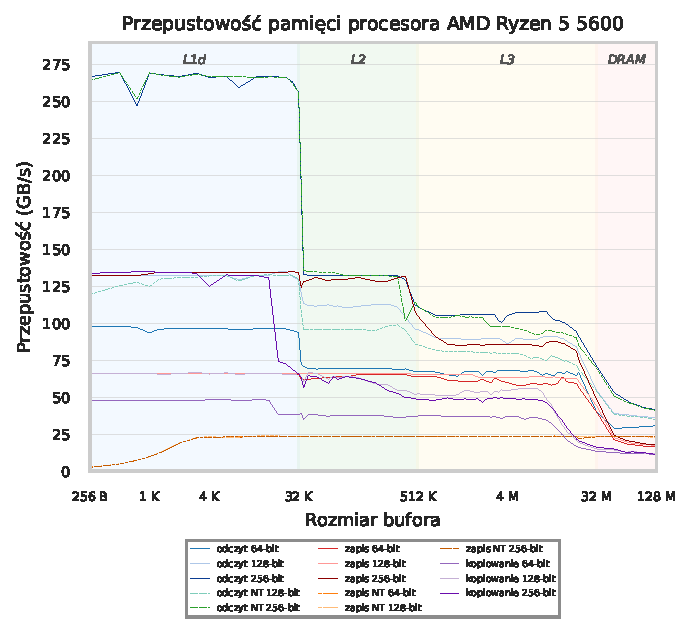
\includegraphics[width=0.82\textwidth]{bandwidth}
\caption{Przepustowość pamięci procesora AMD Ryzen 5 5600 zmierzona narzędziem bandwidth \cite{smith_bandwidth} dla sekwencyjnych odczytów, zapisów, operacji nietymczasowych (ang. \emph{nontemporal}, NT) i kopiowania przy szerokościach 64, 128 i 256 bitów; zacienione obszary odpowiadają poziomom pamięci podręcznej L1d, L2 i L3 oraz pamięci operacyjnej (DRAM)}
\label{rys:bandwidth}
\end{figure}

Oprogramowanie zbudowano w systemie Arch Linux z jądrem w wersji 7.0.11-zen1. Kod źródłowy, napisany zgodnie ze standardem języka C11, skompilowano kompilatorem GCC w wersji 16.1.1. Kompilację prowadzono z zestawem flag dobranych pod procesor docelowy: \texttt{-O3} włącza pełny zakres optymalizacji kompilatora, \texttt{-march=znver3} oraz \texttt{-mtune=znver3} kierują generowaniem i strojeniem kodu pod mikroarchitekturę Zen 3 (między innymi dobór instrukcji oraz model kosztu właściwy dla tego procesora), a \texttt{-mavx2} i \texttt{-mfma} udostępniają instrukcje rozszerzeń AVX2 oraz operację łączonego mnożenia z dodawaniem (ang. \emph{fused multiply-add}, FMA). Pozostałe flagi pełnią rolę pomocniczą: \texttt{-funroll-loops} rozwija pętle, \texttt{-flto} włącza optymalizację międzymodułową w fazie konsolidacji (ang. \emph{link-time optimization}, LTO), a \texttt{-fno-plt} eliminuje pośrednictwo tablicy łączeń procedur przy wywołaniach funkcji zewnętrznych. Zrównoleglenie obliczeń zrealizowano za pomocą interfejsu OpenMP \cite{openmp52}.

Jako punkt odniesienia dla autorskich implementacji posłużyły dojrzałe biblioteki wysokiej wydajności, zbudowane ze źródeł z konfiguracją celu dobraną pod mikroarchitekturę Zen 3 (cel \texttt{CORE\_ZEN} w OpenBLAS, rodzina \texttt{zen3} w AOCL-BLAS): OpenBLAS w wersji 0.3.31 \cite{zhang2012openblas} oraz AOCL-BLAS w wersji 5.2.0 \cite{amd_aocl_blas}, omówione w podrozdziale \ref{sec:blas-implementacje}. Dla iloczynu skalarnego, mnożenia macierzy przez wektor oraz mnożenia dwóch macierzy wykorzystywane są one wprost, a dla splotu --- jako wykonawcy mnożenia macierzy w referencyjnej realizacji im2col $+$ GEMM (podrozdział \ref{sec:splot-im2col}).

\begin{table}[t!]
\centering
\caption{Środowisko testowe --- konfiguracja sprzętowa i programowa (opóźnienia pamięci podręcznej podano w cyklach; przepustowość L1d i L2 wyznaczono teoretycznie, L3 zmierzono empirycznie, a dla pamięci operacyjnej podano pułap teoretyczny; szczyt obliczeniowy podano dla pojedynczego rdzenia przy taktowaniu przyspieszonym 4,4 GHz)}
\label{tab:srodowisko}
\begin{tabular}{l p{0.58\textwidth}}
\hline
\multicolumn{2}{l}{Sprzęt} \\
\hline
Procesor & AMD Ryzen 5 5600 (Zen 3, rodzina 19h) \\
Rdzenie / wątki & 6 / 12 \\
Taktowanie & 3,5 GHz (bazowe), do 4,4 GHz (przyspieszone) \\
Pamięć podręczna L1 & 32 KiB (dane) + 32 KiB (instrukcje) na rdzeń, 8-drożna, 4--8 cykli, 281,6 GB/s (teoret.) \\
Pamięć podręczna L2 & 512 KiB na rdzeń, 8-drożna, $\ge$12 cykli, 140,8 GB/s (teoret.) \\
Pamięć podręczna L3 & 32 MiB współdzielona, 16-drożna, $\approx$47 cykli, $\approx$106 GB/s (zmierz.) \\
Linia pamięci podręcznej & 64 bajty \\
Pamięć operacyjna & 32 GiB DDR4-3200, dwukanałowo (51,2 GB/s teoretycznie) \\
Szczyt obliczeniowy (1 rdzeń) & $\approx$70,4 GFLOP/s (podwójna precyzja), $\approx$140,8 GFLOP/s (pojedyncza) \\
\hline
\multicolumn{2}{l}{Oprogramowanie} \\
\hline
System operacyjny & Arch Linux, jądro 7.0.11-zen1 \\
Kompilator & GCC 16.1.1 \\
Flagi kompilacji & \texttt{-O3 -march=znver3 -mtune=znver3 -mavx2} \texttt{-mfma -funroll-loops -flto -fno-plt} \\
Standard języka & C11 \\
Zrównoleglenie & OpenMP \\
Biblioteki referencyjne & OpenBLAS 0.3.31, AOCL-BLAS 5.2.0 \\
\hline
\end{tabular}
\end{table}

\section{Metodyka pomiarów}
\label{sec:metodyka}

Wszystkie implementacje zmierzono jednolitym protokołem pomiarowym, którego założenia opisano w tym podrozdziale. Celem było uzyskanie wyników stabilnych, powtarzalnych i porównywalnych między implementacjami, a zarazem odpornych na zaburzenia wprowadzane przez system operacyjny oraz na zmienność czasu wykonania pojedynczego wywołania.

Pomiar czasu. Czas mierzono funkcją \texttt{now\_seconds} opartą na wywołaniu systemowym \texttt{clock\_gettime} z zegarem \texttt{CLOCK\_MONOTONIC\_RAW} (listing \ref{lst:pomiar}). Zegar monotoniczny rośnie wyłącznie do przodu i (w odróżnieniu od zegara czasu kalendarzowego) nie podlega skokowym korektom synchronizacji sieciowej (ang. \emph{Network Time Protocol}, NTP) ani regulacji częstotliwości, dzięki czemu różnica dwóch jego odczytów wiernie oddaje rzeczywisty czas, jaki upłynął. Wariant z przyrostkiem \texttt{RAW} pobiera ponadto surowe wskazania sprzętowego źródła czasu, niekorygowane nawet przez płynne dostrajanie zegara. Mierzony jest zatem czas rzeczywisty a nie czas procesora --- z tego względu sensowne są pomiary jednowątkowe z przypięciem do pojedynczego rdzenia.

Liczba iteracji w każdym przebiegu pomiarowym dobierana jest adaptacyjnie. Najpierw wykonuje się kalibrację (pojedyncze wywołanie mierzonego jądra), z której otrzymuje się przybliżony czas jednego wywołania $t_{\mathrm{one}}$. Liczbę iteracji ustala się następnie tak, by przebieg trwał około jednej sekundy (budżet \texttt{BUDGET\_PER\_RUN\_SEC} równy 1 s): przyjmuje się mniejszą z dwóch wartości --- liczby iteracji zadanej w presecie oraz ilorazu budżetu przez $t_{\mathrm{one}}$. Wykonuje się \texttt{NUM\_RUNS} równe pięć takich przebiegów; dla wywołań kosztownych liczba przebiegów jest redukowana (do dwóch, gdy $t_{\mathrm{one}}$ przekracza 0,5 s, oraz do jednego, gdy przekracza 2 s), aby pomiar nie trwał nadmiernie długo. Dla wywołań szybkich, o czasie $t_{\mathrm{one}}$ poniżej 50 ms, poprzedza się przebiegi rozgrzewką (3 lub 10 iteracji, zależnie od jądra), której zadaniem jest sprowadzenie danych i kodu do pamięci podręcznej oraz ustabilizowanie taktowania procesora przed właściwym pomiarem. Na każde pojedyncze wywołanie nałożono twardy limit \texttt{MAX\_SECONDS\_PER\_CALL} równy 20 s, przy czym przypadki, których przewidywany czas przekracza ten limit, są pomijane jeszcze przed pomiarem --- na podstawie mediany zmierzonej dla poprzedniego, mniejszego presetu; ponadto pojedyncze wywołanie kalibracyjne, które samo przekroczy limit, kończy pomiar danego wariantu. Spośród przebiegów raportowana jest mediana wydajności, mniej wrażliwa na pojedyncze zaburzenia niż wartość średnia, wraz z wartością minimalną, maksymalną oraz odchyleniem liczonym względem mediany. Wydajność wyraża się w miliardach operacji zmiennoprzecinkowych na sekundę (ang. \emph{giga floating-point operations per second}, GFLOPS) według wzoru
\[
\mathrm{GFLOPS} = \frac{2 \cdot \mathit{praca} \cdot \mathit{iteracje}}{\mathit{czas} \cdot 10^9},
\]
w którym czynnik 2 odpowiada dwóm działaniom składającym się na pojedynczą operację łączonego mnożenia z dodawaniem (mnożeniu i dodawaniu), a praca oznacza liczbę takich operacji mnożenia z akumulacją wykonywanych w danej operacji. Konkretne wzory na liczbę działań poszczególnych jąder podano przy ich opisach w podrozdziałach \ref{sec:impl-dot}--\ref{sec:impl-conv}.

\begin{lstfloat}[t!]
\begin{lstlisting}[language=C, caption={Funkcja pomiaru czasu oraz uproszczony szkic adaptacyjnej pętli pomiarowej: każdy przebieg trwa około sekundy, a raportowana jest mediana wydajności z \texttt{NUM\_RUNS} przebiegów}, label={lst:pomiar}]
/* Pomiar czasu: zegar monotoniczny odporny na korekty NTP. */
double now_seconds(void) {
    struct timespec ts;
    clock_gettime(CLOCK_MONOTONIC_RAW, &ts);
    return (double)ts.tv_sec + (double)ts.tv_nsec / 1e9;
}

/* Petla pomiarowa: ok. 1 s na przebieg, mediana z NUM_RUNS przebiegow. */
int iters = min(iter_presetu, (int)(BUDGET / t_one));  /* t_one: czas kalibracji */
for (int run = 0; run < NUM_RUNS; run++) {
    double t0 = now_seconds();
    for (int i = 0; i < iters; i++)
        jadro(/* argumenty */);
    double dt = now_seconds() - t0;
    gflops[run] = (2.0 * praca * iters) / (dt * 1e9);
}
double wynik = mediana(gflops, NUM_RUNS);
\end{lstlisting}
\end{lstfloat}

Bufory wejściowe i wynikowe alokowane są z wyrównaniem adresu początkowego za pomocą funkcji \texttt{aligned\_alloc}. Wyrównanie odpowiada wymaganiom instrukcji wektorowych operujących na danych pobieranych z wyrównanych adresów oraz pozwala uniknąć przecinania linii pamięci podręcznej przez przetwarzane bloki danych. Bufory wypełnia się wartościami losowymi o rozkładzie jednostajnym w przedziale $[-1, 1]$. Ziarno generatora liczb pseudolosowych ustalono na stałą wartość (\texttt{srand(42)}), co zapewnia, że przy każdym uruchomieniu wszystkie implementacje otrzymują identyczne dane wejściowe, a wyniki pozostają powtarzalne. We wszystkich pomiarach operacji z parametrami skalarnymi przyjęto $\alpha = 1$ oraz $\beta = 0$.

Dla każdej implementacji wyznacza się maksymalną różnicę bezwzględną jej wyniku względem wyniku implementacji referencyjnej, czyli maksimum modułu różnicy po wszystkich elementach wyniku. Referencję stanowi biblioteka OpenBLAS: dla iloczynu skalarnego, mnożenia macierzy przez wektor oraz mnożenia dwóch macierzy wprost, a dla splotu w referencyjnej realizacji im2col $+$ GEMM. Otrzymany błąd jest raportowany, lecz nie stosuje się sztywnego progu odcięcia, który dyskwalifikowałby implementację. Pozwalało to wychwycić ewentualne rozbieżności numeryczne między implementacjami (naturalne przy zmiennej kolejności sumowania w arytmetyce zmiennoprzecinkowej) i ocenić ich rząd wielkości, nie odrzucając z góry wyników mieszczących się w granicach dokładności obliczeń.

Liczbę wątków obliczeniowych ustala zmienna środowiskowa \texttt{OMP\_NUM\_THREADS}, a jej wartość jest propagowana do bibliotek referencyjnych OpenBLAS oraz AOCL-BLAS poprzez ich interfejsy ustawiania liczby wątków, tak aby wszystkie porównywane implementacje korzystały z tej samej liczby wątków \cite{openmp52}. Pomiary jednowątkowe przeprowadza się z przypięciem procesu do rdzenia o numerze zero (\texttt{taskset -c 0}), co eliminuje migracje wątku między rdzeniami oraz związane z nimi unieważnienia pamięci podręcznej, a pomiary wielowątkowe --- z przypięciem do sześciu rdzeni fizycznych (\texttt{taskset -c 0-5}). Całością pomiarów steruje skrypt \texttt{run\_suite.py}, który dla każdego jądra i każdego trybu wątkowego ustawia odpowiednie przypięcie oraz zmienne środowiskowe, uruchamia program pomiarowy i zbiera jego wyniki.

Rozmiary danych w presetach pomiarowych dobrano tak, aby zbiór roboczy operacji mieścił się kolejno w pamięci podręcznej L1, L2, L3 albo dopiero w pamięci operacyjnej. Pozwala to obserwować, jak wraz z przekraczaniem pojemności kolejnych poziomów hierarchii pamięci zmienia się wydajność --- co wiąże pomiary z modelem roofline oraz hierarchią pamięci omówionymi w rozdziale \ref{chap:hierarchia}, a także z pojęciem intensywności operacyjnej z podrozdziału \ref{sec:blas-poziomy}. Konkretne presety, wraz z wynikającą z nich rezydencją zbioru roboczego w poszczególnych poziomach pamięci, zestawiono w tabelach przy opisach poszczególnych jąder w podrozdziałach \ref{sec:impl-dot}--\ref{sec:impl-conv}. Część presetów leży przy tym dokładnie na granicy pojemności danego poziomu, a niekiedy nieznacznie ją przekracza (gdy do samego zbioru roboczego dochodzą stos, kod i metadane), dlatego deklarowaną rezydencję należy traktować jako przybliżoną.

\section{Iloczyn skalarny}
\label{sec:impl-dot}

Iloczyn skalarny dwóch wektorów o długości $N$ wykonuje $N$ operacji mnożenia z akumulacją (wielkość praca we wzorze na wydajność z podrozdziału \ref{sec:metodyka}), czyli $2N$ działań zmiennoprzecinkowych. Implementacje iloczynu skalarnego zmierzono dla czterech rozmiarów wektorów, dobranych tak, aby zbiór roboczy, dwa wektory liczb podwójnej precyzji, po $8$ bajtów na element, mieścił się kolejno w pamięci podręcznej L1d, L2, L3 albo dopiero w pamięci operacyjnej (tabela \ref{tab:dot-presety}).

\begin{table}[t!]
\centering
\caption{Presety pomiarowe iloczynu skalarnego: rozmiar wektorów oraz docelowy poziom hierarchii pamięci, w którym mieści się zbiór roboczy (dwa wektory liczb podwójnej precyzji)}
\label{tab:dot-presety}
\begin{tabular}{llll}
\hline
Preset & Liczba elementów $n$ & Dane (wektory $a$, $b$) & Poziom pamięci \\
\hline
\texttt{l1\_fit} & 2\,048      & $2 \times 16$ KiB $=$ 32 KiB   & L1d \\
\texttt{l2\_fit} & 32\,768     & $2 \times 256$ KiB $=$ 512 KiB & L2 \\
\texttt{l3\_fit} & 2\,097\,152 & $2 \times 16$ MiB $=$ 32 MiB   & L3 \\
\texttt{dram}    & 67\,108\,864 & $2 \times 512$ MiB $=$ 1 GiB  & pamięć operacyjna \\
\hline
\end{tabular}
\end{table}

Kolejne warianty wraz z dodawanymi w nich technikami zestawiono w tabeli \ref{tab:dot-impl}.

Implementacja naiwna (skalarna). Punktem odniesienia jest pojedyncza pętla skalarna sumująca iloczyny odpowiadających sobie składowych obu wektorów do jednej zmiennej akumulującej (listing \ref{lst:dot-naiwny}). Jej zwektoryzowanie pozostawiono kompilatorowi przy włączonych optymalizacjach (\texttt{-O3}) i instrukcjach AVX2 może on samodzielnie przekształcić tę pętlę w postać wektorową, lecz nie ma nad tym procesem jawnej kontroli, w szczególności nad liczbą niezależnych akumulatorów ukrywających opóźnienie potoku.

\begin{lstfloat}[t!]
\begin{lstlisting}[language=C, caption={Iloczyn skalarny, pętla naiwna (skalarna)}, label={lst:dot-naiwny}]
double sum = 0.0;
for (size_t i = 0; i < n; i++)
    sum += a[i] * b[i];
\end{lstlisting}
\end{lstfloat}

Wektoryzacja AVX2 z jednym akumulatorem. Drugi wariant zastępuje pętlę skalarną jawnymi instrukcjami wektorowymi AVX2, zapisanymi za pomocą funkcji wbudowanych (ang. \emph{intrinsics}) \cite{gepner2017avx2}. Obliczenia prowadzi się w jednym 256-bitowym akumulatorze, do którego w każdej iteracji jedna instrukcja FMA (\texttt{\_mm256\_fmadd\_pd}) dolicza iloczyn czterech kolejnych par składowych --- tyle bowiem liczb podwójnej precyzji mieści rejestr YMM (podrozdział \ref{sec:avx}). Po przejściu pętli głównej zawartość akumulatora redukuje się poziomo do pojedynczego skalara, sumując jego cztery składowe, a ewentualne elementy ogona, gdy długość wektora nie jest wielokrotnością czterech, dolicza się w skalarnej pętli resztkowej. Wariant ten cierpi jednak na zasadnicze ograniczenie: kolejne instrukcje FMA dopisują wynik do tego samego akumulatora, tworząc pojedynczy łańcuch zależności. Ponieważ każda z nich musi poczekać na wynik poprzedniej, a opóźnienie pojedynczej operacji FMA na Zen 3 wynosi cztery cykle (podrozdział \ref{sec:avx}), potok jednostek wektorowych nie jest nasycony nawet gdy dane są już w pamięci podręcznej.

Wektoryzacja AVX2 z ośmioma akumulatorami. Wariant trzeci usuwa to ograniczenie kluczową dla wszystkich dalszych jąder techniką prowadzenia obliczeń w wielu niezależnych akumulatorach. Pętla główna wykorzystuje osiem rejestrów akumulujących, a w każdej iteracji wykonuje osiem niezależnych instrukcji FMA, z których każda przetwarza inną czwórkę składowych; w sumie iteracja przetwarza trzydzieści dwa elementy każdego wektora (listing \ref{lst:dot-akum}). Daje to osiem niezależnych łańcuchów operacji FMA, które nie blokują się wzajemnie. Liczba ta wynika z przemnożenia liczby jednostek przez opóźnienie pojedynczej operacji ($2 \times 4 = 8$); poniżej tej granicy potok pozostaje częściowo bezczynny. Po wyczerpaniu pętli głównej osiem akumulatorów sumuje się redukcją drzewiastą parami, na trzech poziomach do jednego rejestru wektorowego, po czym następuje pętla resztkowa przetwarzająca po cztery elementy, redukcja pozioma do skalara oraz skalarny ogon dla pozostałych elementów.

\begin{lstfloat}[t!]
\begin{lstlisting}[language=C, caption={Iloczyn skalarny --- rdzeń wektorowy z ośmioma niezależnymi akumulatorami (AVX2/FMA): osiem łańcuchów FMA po 32 elementy na iterację, redukcja drzewiasta, pętla resztkowa i redukcja pozioma}, label={lst:dot-akum}]
/* Osiem niezaleznych akumulatorow 256-bitowych. */
__m256d s0 = _mm256_setzero_pd();
__m256d s1 = _mm256_setzero_pd();
//...
__m256d s7 = _mm256_setzero_pd();

/* Petla glowna: 32 elementy na iteracje, 8 niezaleznych lancuchow FMA. */
size_t i = 0;
for (; i + 31 < n; i += 32) {
    s0 = _mm256_fmadd_pd(_mm256_loadu_pd(&a[i +  0]), _mm256_loadu_pd(&b[i +  0]), s0);
    s1 = _mm256_fmadd_pd(_mm256_loadu_pd(&a[i +  4]), _mm256_loadu_pd(&b[i +  4]), s1);
    //...
    s7 = _mm256_fmadd_pd(_mm256_loadu_pd(&a[i + 28]), _mm256_loadu_pd(&b[i + 28]), s7);
}

/* Redukcja drzewiasta osmiu akumulatorow do jednego rejestru. */
__m256d t0  = _mm256_add_pd(s0, s1);
__m256d t1  = _mm256_add_pd(s2, s3);
__m256d t2  = _mm256_add_pd(s4, s5);
__m256d t3  = _mm256_add_pd(s6, s7);
__m256d acc = _mm256_add_pd(_mm256_add_pd(t0, t1), _mm256_add_pd(t2, t3));

/* Petla resztkowa: po 4 elementy. */
for (; i + 3 < n; i += 4)
    acc = _mm256_fmadd_pd(_mm256_loadu_pd(&a[i]), _mm256_loadu_pd(&b[i]), acc);

/* Redukcja pozioma do skalara, nastepnie skalarny ogon. */
double sum = hsum_pd(acc);
for (; i < n; i++)
    sum += a[i] * b[i];
\end{lstlisting}
\end{lstfloat}

Zrównoleglenie OpenMP. Ostatni wariant autorski rozdziela pracę między wątki za pomocą interfejsu OpenMP \cite{openmp52}. Zakres wektora dzieli się ręcznie na rozłączne fragmenty bez konstrukcji \texttt{parallel for}: każdy wątek na podstawie swojego numeru oraz całkowitej liczby wątków wyznacza początek i koniec przypadającego mu fragmentu i liczy iloczyn skalarny tej części opisanym wyżej jądrem ośmioakumulatorowym (listing \ref{lst:dot-omp}). Wyniki cząstkowe wszystkich wątków łączy klauzula redukcji \texttt{reduction(+:total)}, sumując je w jeden skalar. Zrównoleglenie ma sens jedynie dla danych dużych: dla wektorów małych dominuje narzut tworzenia i synchronizacji wątków, a dla wektorów bardzo dużych ograniczonych przepustowością pamięci operacyjnej wiele wątków rywalizuje o tę samą, wspólną przepustowość, wobec czego przyśpieszenie szybko się nasyca i pozostaje ograniczone tą przepustowością, a nie liczbą wątków.

\begin{lstfloat}[t!]
\begin{lstlisting}[language=C, caption={Iloczyn skalarny --- region równoległy OpenMP: ręczny podział zakresu wektora na rozłączne fragmenty i redukcja wyników cząstkowych}, label={lst:dot-omp}]
double total = 0.0;
#pragma omp parallel reduction(+:total)
{
    int    nt    = omp_get_num_threads();
    int    tid   = omp_get_thread_num();
    size_t chunk = n / nt;
    size_t start = (size_t)tid * chunk;
    size_t end   = (tid == nt - 1) ? n : start + chunk;
    /* iloczyn skalarny fragmentu wariantem 8-akumulatorowym */
    total = dot_fragment(a + start, b + start, end - start);
}
/* wynik: total */
\end{lstlisting}
\end{lstfloat}

Biblioteki referencyjne. Jako odniesienie posłużyły dwie dojrzałe biblioteki opisane w podrozdziale \ref{sec:blas-implementacje}: OpenBLAS \cite{zhang2012openblas}, wywoływana przez interfejs C funkcją \texttt{cblas\_ddot}, oraz AOCL-BLAS \cite{amd_aocl_blas}, wywoływana przez interfejs Fortranu funkcją \texttt{ddot\_}. 

\begin{table}[t!]
\centering
\caption{Implementacje iloczynu skalarnego oraz techniki optymalizacji dodawane w kolejnych wariantach}
\label{tab:dot-impl}
\begin{tabular}{p{0.40\textwidth} p{0.52\textwidth}}
\hline
Implementacja & Dodana technika optymalizacji \\
\hline
naiwna (skalarna) & pętla skalarna; punkt odniesienia, zdana na automatyczną wektoryzację kompilatora \\
wektoryzacja AVX2 (1 akumulator) & jawne instrukcje AVX2 i FMA, 4 elementy na iterację; redukcja pozioma i skalarny ogon \\
wektoryzacja AVX2 (8 akumulatorów) & 8 niezależnych łańcuchów FMA (32 elementy na iterację) --- ukrycie opóźnienia FMA; redukcja drzewiasta \\
zrównoleglenie OpenMP & ręczny podział zakresu na wątki i redukcja, na jądrze ośmioakumulatorowym \\
OpenBLAS / AOCL-BLAS & biblioteki referencyjne (\texttt{cblas\_ddot} / \texttt{ddot\_}) \\
\hline
\end{tabular}
\end{table}

\section{Mnożenie macierzy przez wektor}
\label{sec:impl-gemv}

Mnożenie macierzy o wymiarach $M \times N$ przez wektor wykonuje $M N$ operacji mnożenia z akumulacją (wielkość praca we wzorze na wydajność z podrozdziału \ref{sec:metodyka}), czyli $2 M N$ działań zmiennoprzecinkowych. W ujęciu wierszowym, przyjętym we wszystkich opisywanych implementacjach, każda składowa wyniku jest iloczynem skalarnym odpowiedniego wiersza macierzy $A$ z wektorem $\mathbf{x}$. Z tego względu wariant naiwny i podstawowa wektoryzacja powielają techniki przedstawione szczegółowo dla iloczynu skalarnego; poniżej omawia się je skrótowo, kładąc nacisk na techniki swoiste dla GEMV przede wszystkim na reużycie wektora $\mathbf{x}$ wspólnego dla wielu wierszy oraz na blokowanie pamięci podręcznej dla dużych macierzy. Implementacje zmierzono dla sześciu presetów dobranych tak, aby zbiór roboczy mieścił się w kolejnych poziomach hierarchii pamięci (tabela \ref{tab:gemv-presety}); operację zaimplementowano w siedmiu autorskich wariantach o narastającym stopniu optymalizacji, zestawionych wraz z dodawanymi technikami w tabeli \ref{tab:gemv-impl}, i porównano z dwiema bibliotekami referencyjnymi.

\begin{table}[t!]
\centering
\caption{Presety pomiarowe mnożenia macierzy przez wektor: wymiary macierzy oraz docelowy poziom hierarchii pamięci, w którym mieści się zbiór roboczy (macierz $A$ oraz wektory $\mathbf{x}$, $\mathbf{y}$ liczb podwójnej precyzji)}
\label{tab:gemv-presety}
\begin{tabular}{llll}
\hline
Preset & Wiersze $\times$ kolumny & Zbiór roboczy ($A$, $\mathbf{x}$, $\mathbf{y}$) & Poziom pamięci \\
\hline
\texttt{tiny}   & $64 \times 64$     & $\approx 33$ KiB  & L1d \\
\texttt{small}  & $256 \times 256$   & $\approx 516$ KiB & L2 \\
\texttt{medium} & $1024 \times 1024$ & $\approx 8$ MiB   & L3 \\
\texttt{large}  & $4096 \times 4096$ & $\approx 128$ MiB & pamięć operacyjna \\
\texttt{wide}   & $256 \times 8192$  & $\approx 16$ MiB  & L3 / pamięć operacyjna \\
\texttt{tall}   & $8192 \times 256$  & $\approx 16$ MiB  & L3 / pamięć operacyjna \\
\hline
\end{tabular}
\end{table}

Implementacja naiwna (skalarna). Punktem odniesienia jest podwójna pętla, w której każdy wiersz macierzy liczony jest jako skalarny iloczyn z wektorem $\mathbf{x}$ akumulującą sumę, jak w naiwnym iloczynie skalarnym.

Wektoryzacja AVX2. Drugi wariant przetwarza każdy wiersz jawnymi instrukcjami wektorowymi AVX2 \cite{gepner2017avx2}, używając dwóch 256-bitowych akumulatorów i ośmiu kolumn na iterację. Inaczej niż w jądrach dalszych, mnożenie i dodawanie wykonywane są tu osobnymi instrukcjami, jeszcze bez operacji FMA. Każdy wiersz kończy się redukcją poziomą akumulatorów do skalara oraz skalarną pętlą resztkową analogicznie do wariantu wektorowego iloczynu skalarnego (podrozdział \ref{sec:impl-dot}).

Prefetch programowy i dostępy wyrównane. Wariant trzeci uzupełnia poprzedni o jawny prefetch programowy (\texttt{\_mm\_prefetch}), sprowadzający z wyprzedzeniem kolejne wiersze macierzy $A$, zanim staną się potrzebne. Ta implementacja ma charakter demonstracyjny, gdyż dla regularnych, strumieniowych wzorców dostępu (jak sekwencyjne przemiatanie macierzy) prefetch programowy zwykle nie przynosi dodatkowych korzyści, zgodnie z informacjami w rozdziale \ref{chap:lokalnosc}.

Jądro FMA z blokowaniem 4-wierszowym. Czwarty wariant wprowadza technikę swoistą dla GEMV: przetwarzanie czterech wierszy macierzy naraz. Cztery kolejne wiersze $\mathbf{a}_0, \dots, \mathbf{a}_3$ przechodzone są wspólnie, a wczytany fragment wektora $\mathbf{x}$ jest reużywany we wszystkich czterech wierszach, zanim zostanie zastąpiony następnym. Dzięki temu wektor $\mathbf{x}$ jedyna dana podlegająca reużyciu w tej operacji sprowadzany jest z pamięci czterokrotnie rzadziej, co bezpośrednio zmniejsza ruch pamięci. Obliczenia prowadzi się instrukcjami FMA, po jednym akumulatorze na wiersz, co daje cztery niezależne łańcuchy zależności.

Podwójne akumulatory na wiersz. Wariant piąty (autorskie jądro jednowątkowe) zachowuje blokowanie 4-wierszowe z reużyciem wektora $\mathbf{x}$, lecz prowadzi obliczenia w dwóch akumulatorach na każdy z czterech wierszy, co daje osiem niezależnych łańcuchów FMA (listing \ref{lst:gemv-v3}) --- dokładnie tyle, ile potrzeba do nasycenia obu jednostek FMA mikroarchitektury Zen 3. Pętla główna przetwarza szesnaście kolumn na iterację; pary akumulatorów każdego wiersza sumuje się następnie do jednego, po czym wykonywane są pętle resztkowe (po osiem, cztery oraz pojedyncze kolumny) i redukcja pozioma do składowych wyniku.

\begin{lstfloat}[t!]
\begin{lstlisting}[language=C, caption={Mnożenie macierzy przez wektor --- gorąca pętla jądra 4-wierszowego z podwójnymi akumulatorami (AVX2/FMA): wektor x wczytywany raz i reużyty w czterech wierszach, osiem niezależnych łańcuchów FMA po 16 kolumn na iterację}, label={lst:gemv-v3}]
/* Dwa akumulatory na kazdy z czterech wierszy: 8 lancuchow FMA. */
__m256d sum0a = _mm256_setzero_pd(), sum0b = _mm256_setzero_pd();
__m256d sum1a = _mm256_setzero_pd(), sum1b = _mm256_setzero_pd();
__m256d sum2a = _mm256_setzero_pd(), sum2b = _mm256_setzero_pd();
__m256d sum3a = _mm256_setzero_pd(), sum3b = _mm256_setzero_pd();

/* Petla glowna: 16 kolumn na iteracje. */
int j = 0;
for (; j + 15 < cols; j += 16) {
    /* Cztery rejestry x wczytane RAZ, reuzyte w czterech wierszach. */
    __m256d x0 = _mm256_load_pd(&x[j]);
    __m256d x1 = _mm256_load_pd(&x[j + 4]);
    __m256d x2 = _mm256_load_pd(&x[j + 8]);
    __m256d x3 = _mm256_load_pd(&x[j + 12]);

    sum0a = _mm256_fmadd_pd(_mm256_load_pd(&a0[j]),      x0, sum0a);
    sum0b = _mm256_fmadd_pd(_mm256_load_pd(&a0[j + 4]),  x1, sum0b);
    sum0a = _mm256_fmadd_pd(_mm256_load_pd(&a0[j + 8]),  x2, sum0a);
    sum0b = _mm256_fmadd_pd(_mm256_load_pd(&a0[j + 12]), x3, sum0b);

    sum1a = _mm256_fmadd_pd(_mm256_load_pd(&a1[j]),      x0, sum1a);
    sum1b = _mm256_fmadd_pd(_mm256_load_pd(&a1[j + 4]),  x1, sum1b);
    sum1a = _mm256_fmadd_pd(_mm256_load_pd(&a1[j + 8]),  x2, sum1a);
    sum1b = _mm256_fmadd_pd(_mm256_load_pd(&a1[j + 12]), x3, sum1b);

    sum2a = _mm256_fmadd_pd(_mm256_load_pd(&a2[j]),      x0, sum2a);
    sum2b = _mm256_fmadd_pd(_mm256_load_pd(&a2[j + 4]),  x1, sum2b);
    sum2a = _mm256_fmadd_pd(_mm256_load_pd(&a2[j + 8]),  x2, sum2a);
    sum2b = _mm256_fmadd_pd(_mm256_load_pd(&a2[j + 12]), x3, sum2b);

    sum3a = _mm256_fmadd_pd(_mm256_load_pd(&a3[j]),      x0, sum3a);
    sum3b = _mm256_fmadd_pd(_mm256_load_pd(&a3[j + 4]),  x1, sum3b);
    sum3a = _mm256_fmadd_pd(_mm256_load_pd(&a3[j + 8]),  x2, sum3a);
    sum3b = _mm256_fmadd_pd(_mm256_load_pd(&a3[j + 12]), x3, sum3b);
}
/* Suma par akumulatorow do jednego na wiersz, petle resztkowe (8/4/skalar),
   redukcja pozioma do y[0..3]. */
\end{lstlisting}
\end{lstfloat}

Blokowanie pamięci podręcznej. Dla macierzy zbyt dużych, by zmieścić się w pamięci podręcznej, samo reużycie wektora $\mathbf{x}$ w rejestrach nie wystarcza --- jego fragmenty wypadają z pamięci podręcznej, zanim zostaną ponownie użyte w dalszych wierszach. Wariant szósty stosuje zatem blokowanie (kafelkowanie) wierszy i kolumn: obliczenie dzieli się na kafle, w obrębie których fragment macierzy $A$ oraz odpowiadający mu fragment wektora $\mathbf{x}$ pozostają rezydentne w danym poziomie pamięci podręcznej (listing \ref{lst:gemv-blok}). Rozmiary bloków dobrano poza pomiarem poprzez strojenie, empirycznie, osobno dla pamięci podręcznej L1, L2 i L3, a dyspozytor wybiera odpowiedni zestaw na podstawie rozmiaru zbioru roboczego operacji, włączając przy większych blokach prefetch programowy. Wewnątrz kafla działa to samo jądro 4-wierszowe z reużyciem wektora $\mathbf{x}$, lecz z jednym akumulatorem na wiersz --- a więc czterema łańcuchami FMA zamiast ośmiu. Wariant ten kładzie zatem nacisk na lokalność danych kosztem mniejszej liczby równoległych łańcuchów obliczeniowych.

\begin{lstfloat}[t!]
\begin{lstlisting}[language=C, caption={Mnożenie macierzy przez wektor --- szkic blokowania pamięci podręcznej: dyspozytor dobiera rozmiary bloków wg rozmiaru zbioru roboczego, a zagnieżdżone pętle przebiegają kafle kolumn i wierszy}, label={lst:gemv-blok}]
/* Dyspozytor: rozmiary blokow wg rozmiaru zbioru roboczego. */
size_t ws = (size_t)rows * cols * 8 + (cols + rows) * 8;
int row_blk, col_blk;
if      (ws <= L1_THRESHOLD) { row_blk =  64; col_blk = 512; } /* L1 */
else if (ws <= L2_THRESHOLD) { row_blk = 128; col_blk = 256; } /* L2 */
else                         { row_blk =  64; col_blk = 512; } /* L3 */

/* Kafelkowanie: kafel A i fragment x rezydentne w danym poziomie cache. */
for (int jj = 0; jj < cols; jj += col_blk)
    for (int ii = 0; ii < rows; ii += row_blk)
        /* jadro 4-wierszowe z reuzyciem x (1 akumulator/wiersz) */
        gemv_kernel_4rows(ii, jj, row_blk, col_blk, A, x, y, alpha);
\end{lstlisting}
\end{lstfloat}

Zrównoleglenie OpenMP. Ostatni wariant autorski zrównolegla jądro ośmioakumulatorowe za pomocą interfejsu OpenMP \cite{openmp52}. Wiersze macierzy dzieli się ręcznie na rozłączne fragmenty między wątki z granicami wyrównanymi do czterech wierszy, zgodnie z blokowaniem 4-wierszowym jądra. Każdy wątek zapisuje wówczas rozłączny fragment wektora wynikowego $\mathbf{y}$, co eliminuje fałszywe współdzielenie. Zrównoleglenie uruchamiane jest jednak warunkowo, w zależności od rozmiaru zadania: region równoległy tworzony jest tylko wtedy, gdy macierz ma co najmniej $128$ wierszy, a liczba jej elementów mieści się w przedziale od $65\,536$ do $8\,388\,608$; poza tym przedziałem obliczenie wykonuje się sekwencyjnie. Dolny próg odcina najmniejsze macierze, dla których narzut tworzenia i synchronizacji wątków przeważa nad zyskiem, natomiast górny --- macierze na tyle duże, że i tak ogranicza je wspólna dla wszystkich rdzeni przepustowość pamięci operacyjnej, wobec czego zrównoleglenie nie podnosi wydajności, a jedynie dokłada narzut koordynacji. W konsekwencji dla najmniejszego (\texttt{tiny}) oraz największego (\texttt{large}) spośród badanych presetów wariant ten wykonuje się w istocie ścieżką sekwencyjną --- co należy mieć na uwadze przy interpretacji jego wyników w rozdziale \ref{chap:wyniki}.

Biblioteki referencyjne. Jako odniesienie posłużyły dwie biblioteki: OpenBLAS \cite{zhang2012openblas}, wywoływana przez interfejs C funkcją \texttt{cblas\_dgemv} z układem wierszowym macierzy, oraz AOCL-BLAS \cite{amd_aocl_blas}, wywoływana przez interfejs Fortran funkcją \texttt{dgemv\_}. Ponieważ Fortran posługuje się układem kolumnowym, macierz przechowywaną wierszowo przekazuje się do AOCL-BLAS z żądaniem transpozycji --- co odpowiada temu samemu mnożeniu w układzie wierszowym.

\begin{table}[t!]
\centering
\caption{Implementacje mnożenia macierzy przez wektor oraz techniki optymalizacji dodawane w kolejnych wariantach}
\label{tab:gemv-impl}
\begin{tabular}{p{0.40\textwidth} p{0.52\textwidth}}
\hline
Implementacja & Dodana technika optymalizacji \\
\hline
naiwna (skalarna) & podwójna pętla, każdy wiersz jako iloczyn skalarny z $\mathbf{x}$; punkt odniesienia \\
wektoryzacja AVX2 & 2 akumulatory na wiersz, mnożenie i dodawanie osobno (bez FMA), 8 kolumn na iterację \\
$+$ prefetch programowy & sprowadzanie $A$ i $\mathbf{x}$ z wyprzedzeniem; dostępy wektorowe wyrównane \\
jądro FMA, blokowanie 4-wierszowe & FMA; 4 wiersze naraz z reużyciem wektora $\mathbf{x}$; 4 niezależne łańcuchy \\
$+$ podwójne akumulatory na wiersz & 8 niezależnych łańcuchów FMA, 16 kolumn na iterację --- nasycenie jednostek FMA \\
$+$ blokowanie pamięci podręcznej & kafelkowanie wierszy i kolumn, prefetch oraz dyspozytor wg rozmiaru (bloki strojone pod L1/L2/L3) \\
zrównoleglenie OpenMP & ręczny podział wierszy na wątki (fragmenty 4-wierszowe), bez fałszywego współdzielenia $\mathbf{y}$; równoległość warunkowa (tylko dla $\ge 128$ wierszy oraz $65\,536$--$8\,388\,608$ elementów) \\
OpenBLAS / AOCL-BLAS & biblioteki referencyjne (\texttt{cblas\_dgemv} / \texttt{dgemv\_}) \\
\hline
\end{tabular}
\end{table}

\section{Mnożenie macierzy}
\label{sec:impl-gemm}

Mnożenie macierzy o wymiarach $M \times K$ przez macierz $K \times N$ wykonuje $M N K$ operacji mnożenia z akumulacją (wielkość praca we wzorze na wydajność z podrozdziału \ref{sec:metodyka}), czyli $2 M N K$ działań zmiennoprzecinkowych. GEMM, inaczej niż iloczyn skalarny i mnożenie macierzy przez wektor jest operacją ograniczoną mocą obliczeniową, dla której decydujące znaczenie ma utrzymanie jednostek FMA w ciągłej pracy. Wymaga to dwóch technik lokalności danych: blokowania (kafelkowania) dopasowanego do pojemności kolejnych poziomów pamięci podręcznej oraz pakowania. Kanoniczną organizację takiego obliczenia przedstawiono w podrozdziale \ref{sec:blas-implementacje}; opisywane niżej warianty stopniowo do niej zmierzają, a następnie dostrajają mikrojądro do architektury Zen 3. Implementacje zmierzono dla siedmiu presetów obejmujących macierze rezydentne w kolejnych poziomach pamięci oraz kształty niekwadratowe (tabela \ref{tab:gemm-presety}); operację zaimplementowano w dwunastu autorskich wariantach o narastającym stopniu optymalizacji, zestawionych wraz z dodawanymi technikami w tabeli \ref{tab:gemm-impl}, i porównano z dwiema bibliotekami referencyjnymi.

\begin{table}[t!]
\centering
\caption{Presety pomiarowe mnożenia dwóch macierzy: wymiary $M \times N \times K$ oraz charakterystyka zadania. Macierze przechowywane są w liczbach podwójnej precyzji, a rozmiary dobrano tak, aby objąć rezydencję w kolejnych poziomach pamięci oraz kształty niekwadratowe}
\label{tab:gemm-presety}
\begin{tabular}{p{0.16\textwidth} p{0.26\textwidth} p{0.46\textwidth}}
\hline
Preset & $M \times N \times K$ & Charakterystyka \\
\hline
\texttt{tiny}   & $64 \times 64 \times 64$       & bardzo małe; ścieżka bez packingu \\
\texttt{small}  & $256 \times 256 \times 256$    & rezydencja rzędu pamięci podręcznej L2 \\
\texttt{medium} & $1024 \times 1024 \times 1024$ & duże (L3 / pamięć operacyjna) \\
\texttt{large}  & $4096 \times 4096 \times 4096$ & bardzo duże (pamięć operacyjna) \\
\texttt{rank\_k} & $2048 \times 2048 \times 128$ & małe $K$ (aktualizacja niskiego rzędu) \\
\texttt{tall\_K} & $128 \times 2048 \times 2048$ & duże $K$, małe $M$ \\
\texttt{odd}    & $1252 \times 1500 \times 257$  & wymiary niestandardowe (brzeg dla kafelka $6 \times 8$) \\
\hline
\end{tabular}
\end{table}

Implementacja naiwna (trzy pętle). Punktem odniesienia jest klasyczna potrójna pętla w kolejności $i$--$j$--$k$. W tej kolejności pętla najbardziej wewnętrzna przebiega wskaźnik $k$, co przy układzie wierszowym oznacza dostęp do macierzy $B$ z krokiem równym jej liczbie kolumn, a więc nieciągły, wrogi pamięci podręcznej i niepodatny na wektoryzację.

Zmiana kolejności pętli (i-k-j). Drugi wariant zmienia kolejność zagnieżdżenia na $i$--$k$--$j$, pozostawiając ten sam zbiór działań. Pętla najbardziej wewnętrzna przebiega teraz wskaźnik $j$, a więc kolejne, ciągłe elementy wiersza macierzy $B$ oraz wiersza wyniku $C$; element $A_{ik}$ jest w niej niezmiennikiem, dzięki czemu można go wynieść przed pętlę i wczytać tylko raz (listing \ref{lst:gemm-ikj}). Jednostkowy, ciągły dostęp w pętli wewnętrznej naprawia lokalność przestrzenną i czyni tę pętlę podatną na wektoryzację jest to klasyczna transformacja kolejności pętli.

\begin{lstfloat}[t!]
\begin{lstlisting}[language=C, caption={Mnożenie dwóch macierzy: element \texttt{A[i][k]} wyniesiony przed pętlę wewnętrzną, która przebiega ciągłe elementy wiersza B i wiersza C}, label={lst:gemm-ikj}]
for (int i = 0; i < M; i++) {
    for (int k = 0; k < K; k++) {
        double a_ik = alpha * A[i * K + k];  /* niezmiennik j */
        const double* b_row = &B[k * N];      /* ciagly wiersz B */
        double* c_row = &C[i * N];            /* ciagly wiersz C */
        for (int j = 0; j < N; j++) {
            c_row[j] += a_ik * b_row[j];      /* dostep ciagly */
        }
    }
}
\end{lstlisting}
\end{lstfloat}

Blokowanie pamięci podręcznej. Sama poprawna kolejność pętli nie wystarcza dla dużych macierzy: gdy wiersze macierzy $B$ są na tyle długie, że wypierają się nawzajem z pamięci podręcznej, zanim zostaną ponownie użyte dla kolejnego wiersza $A$, każdy element $B$ trzeba sprowadzać z pamięci wielokrotnie. Trzeci wariant stosuje zatem blokowanie (kafelkowanie): obliczenie dzieli się na bloki o wymiarach tak dobranych, aby przetwarzane podmacierze $A$, $B$ i $C$ pozostawały rezydentne w pamięci podręcznej przez czas ich wielokrotnego użycia. Wewnątrz bloku pracuje pętla $i$--$k$--$j$ z poprzedniego wariantu; blokowanie ogranicza ruch między pamięcią operacyjną a procesorem do niezbędnego minimum, zwiększając reużycie raz sprowadzonych danych.

Packing i mikrojądro $6 \times 8$. Czwarty wariant wprowadza pełną anatomię wydajnego mnożenia macierzy pięć zagnieżdżonych pętli z packingiem, opisaną w podrozdziale \ref{sec:blas-implementacje} \cite{goto2008anatomy,vanzee2015blis}. Packing pełni dwojaką rolę: po pierwsze, układa elementy paneli dokładnie w kolejności, w jakiej odczytuje je mikrojądro, dzięki czemu wszystkie jego dostępy do pamięci są ciągłe i wyrównane do granicy rejestru; po drugie, eliminuje chybienia konfliktowe pamięci podręcznej, gdyż ciągły bufor nie powiela tych samych zbiorów asocjacyjnych co rozproszone wiersze macierzy źródłowej (rozdział \ref{chap:lokalnosc}). Wariant ten korzysta z mikrojądra o wymiarach $M_R = 6$, $N_R = 8$ domyślnego kafelka frameworku BLIS dla całej rodziny Haswell oraz Zen, dobranego pod przenośność, a nie pod optimum konkretnej mikroarchitektury \cite{vanzee2015blis}.

Mikrojądro $4 \times 12$ Piąty wariant zastępuje kafelek $6 \times 8$ kafelkiem o wymiarach $M_R = 4$, $N_R = 12$, optymalnym dla mikroarchitektury Zen 3. Wybór ten wynika z rachunku liczby mikrooperacji i bilansu rejestrów wektorowych. Mikrojądro utrzymuje $M_R \cdot N_R / 4$ akumulatorów (po jednym 256-bitowym rejestrze YMM na cztery sąsiednie elementy wyniku), jeden rejestr na powielony skalar z macierzy $A$ oraz $N_R / 4$ rejestrów na wektory z macierzy $B$. Liczba akumulatorów musi przy tym dać co najmniej osiem niezależnych łańcuchów zależności, aby ukryć czterocyklowe opóźnienie instrukcji FMA, a łączna liczba rejestrów nie może przekroczyć szesnastu architektonicznych rejestrów YMM dostępnych w AVX2 (podrozdział \ref{sec:rejestry}) \cite{fog_microarchitecture}. Tabela \ref{tab:gemm-tile} zestawia rozważane kafelki wobec obu ograniczeń. Kafelek $4 \times 12$ daje $12$ akumulatorów (a więc dwanaście łańcuchów, znacznie ponad wymagane osiem), $1$ rejestr powielenia $A$ oraz $3$ wektory $B$, co w sumie wynosi dokładnie szesnaście rejestrów YMM --- wypełnia więc cały plik rejestrów architektonicznych. Wymaga przy tym siedmiu odczytów wektorowych na dwanaście instrukcji FMA w każdej iteracji pętli po $K$ (cztery powielenia $A$ i trzy odczyty $B$), czyli $0{,}58$ odczytu na FMA, podczas gdy kafelek $6 \times 8$ przy tych samych dwunastu akumulatorach wymaga ośmiu odczytów ($0{,}67$ na FMA). Niższa liczba odczytów na FMA pozostawia większy zapas na jednostkach odczytu, który amortyzuje konflikty dostępu do pamięci podręcznej i rywalizację o porty z prefetcherem sprzętowym.

\begin{table}[t!]
\centering
\caption{Przestrzeń projektowa kafelków mikrojądra $M_R \times N_R$ dla AVX2 (16 rejestrów YMM, opóźnienie FMA 4 cykle, dwie jednostki FMA). Liczba rejestrów obejmuje akumulatory, jeden rejestr powielenia $A$ oraz $N_R/4$ wektorów $B$; kafelki o ponad 16 rejestrach wymuszają spilling}
\label{tab:gemm-tile}
\small
\setlength{\tabcolsep}{4pt}
\begin{tabular}{ccccccp{0.26\textwidth}}
\hline
$M_R \times N_R$ & Akum. & YMM & Odcz./iter. & FMA/iter. & Odcz./FMA & Uwaga \\
\hline
$2 \times 8$  & 4  & 7  & 4 & 4  & $1{,}00$ & za mało łańcuchów (potrzeba $\ge 8$) \\
$4 \times 8$  & 8  & 11 & 6 & 8  & $0{,}75$ & 8 łańcuchów, 5 rejestrów wolnych \\
$3 \times 12$ & 9  & 13 & 6 & 9  & $0{,}67$ & tuż powyżej minimum łańcuchów \\
$6 \times 8$  & 12 & 15 & 8 & 12 & $0{,}67$ & kafelek domyślny BLIS (przenośność) \\
$\mathbf{4 \times 12}$ & \textbf{12} & \textbf{16} & \textbf{7} & \textbf{12} & $\mathbf{0{,}58}$ & \textbf{optimum --- wypełnia plik rejestrów} \\
$6 \times 12$ & 18 & --- & --- & --- & --- & spilling ($> 16$ YMM) \\
$8 \times 8$  & 16 & --- & --- & --- & --- & spilling \\
\hline
\end{tabular}
\end{table}

Rozmiary bloków ścieżki $4 \times 12$ dobrano tak, aby pakowane panele były rezydentne w kolejnych poziomach pamięci podręcznej (tabela \ref{tab:gemm-bloki}). Przy $K_C = 240$ mikropanel macierzy $A$ o wymiarach $M_R \times K_C$ zajmuje $4 \cdot 240 \cdot 8 \approx 7{,}5$ KiB i mieści się swobodnie w pamięci podręcznej L1 danych ($32$ KiB). Przy $M_C = 192$ cały panel macierzy $A$ o wymiarach $M_C \times K_C$ zajmuje $192 \cdot 240 \cdot 8 \approx 360$ KiB i mieści się w pamięci podręcznej L2 ($512$ KiB) z zapasem na rezydentny pasek macierzy $B$ oraz na bufory zapisu. Przy $N_C = 4080$ panel macierzy $B$ o wymiarach $K_C \times N_C$ zajmuje $240 \cdot 4080 \cdot 8 \approx 7{,}5$ MiB i mieści się we współdzielonej pamięci podręcznej L3 ($32$ MiB) nawet wtedy, gdy korzysta z niego kilka rdzeni. Tabela \ref{tab:gemm-bloki} podaje także alokację rejestrów YMM w mikrojądrze $4 \times 12$.

\begin{table}[t!]
\centering
\caption{Bloki oraz alokacja rejestrów ścieżki $4 \times 12$. Po lewej --- rozmiary bloków packingu wraz z docelowym poziomem rezydencji; po prawej --- przypisanie szesnastu rejestrów YMM rolom w mikrojądrze}
\label{tab:gemm-bloki}
\begin{tabular}{p{0.46\textwidth} p{0.46\textwidth}}
\hline
Blok / panel & Rejestr YMM --- rola \\
\hline
$M_R = 4$, $N_R = 12$ (kafelek) & \texttt{ymm0} --- powielony skalar z $A$ \\
$K_C = 240$: mikropanel $A$ $\approx 7{,}5$ KiB (L1d) & \texttt{ymm1}--\texttt{ymm3} --- 3 wektory $B$ (12 kolumn) \\
$M_C = 192$: panel $A$ $\approx 360$ KiB (L2) & \texttt{ymm4}--\texttt{ymm15} --- 12 akumulatorów \\
$N_C = 4080$: panel $B$ $\approx 7{,}5$ MiB (L3) & \quad (4 wiersze $\times$ 3 grupy kolumn) \\
\hline
\end{tabular}
\end{table}

Wypełnienie całego pliku rejestrów ma istotną konsekwencję dla sposobu zapisania mikrojądra. Dwanaście akumulatorów, jeden rejestr powielenia $A$ oraz trzy wektory $B$ dają dokładnie szesnaście jednocześnie żywych wartości --- a więc cały zbiór rejestrów architektonicznych YMM (podrozdział \ref{sec:rejestry}). Każda dodatkowa wartość tymczasowa, którą kompilator zechce utrzymać w rejestrze (na przykład zmaterializowana stała zerowa służąca do wyzerowania akumulatorów), podnosi liczbę żywych wartości do siedemnastu i wymusza spilling, czyli odesłanie części akumulatorów na stos. W napisanej z czystych funkcji wbudowanych (ang. \emph{intrinsics}) wersji jądra kompilator GCC w wersji 16.1.1 faktycznie wykorzystał rejestr na stałą zerową i w konsekwencji odesłał część akumulatorów na stos; potwierdziła to deasemblacja narzędziem \texttt{objdump}, w której pętla po $K$ zawierała pamięciowe formy instrukcji \texttt{vfmadd213pd} z operandem adresowanym względem wskaźnika ramki stosu oraz zapisy \texttt{vmovapd} na stos w każdej iteracji. Każdy odesłany akumulator wprowadza wówczas do każdej iteracji dodatkowy odczyt i zapis pamięci, niwecząc przewagę kafelka $4 \times 12$ wynikającą z niższej liczby odczytów na FMA.

Rozwiązaniem jest zapisanie pętli po $K$ w asemblerze, w którym każdej roli przypisuje się z góry konkretny rejestr (\texttt{ymm0} --- powielony skalar $A$, \texttt{ymm1}--\texttt{ymm3} --- wektory $B$, \texttt{ymm4}--\texttt{ymm15} --- dwanaście akumulatorów), odbierając kompilatorowi swobodę wprowadzania jakichkolwiek wartości tymczasowych w gorącej pętli (listing \ref{lst:gemm-asm}). Argument przemawiający za tym rozwiązaniem ma charakter architektoniczny, niezależny od wersji kompilatora: szesnaście rejestrów YMM to stała cecha AVX2, a kafelek $4 \times 12$ wykorzystuje ich dokładnie tyle, więc żadna wersja kompilatora nie dysponuje rejestrem zapasowym, którego fizycznie nie ma. Do tego samego wniosku doszli autorzy bibliotek OpenBLAS oraz AOCL-BLAS, których jądra mnożenia macierzy dla rodziny Zen są z tego właśnie powodu pisane w ręcznym asemblerze \cite{zhang2012openblas,vanzee2015blis}. Zmierzone skutki spillingu --- spadek wydajności wariantu z funkcji wbudowanych (w tabelach wyników jako mikrojądro $4 \times 12$ z funkcji wbudowanych) względem asemblerowego --- omówiono w rozdziale poświęconym wynikom.

\begin{lstfloat}[t!]
\begin{lstlisting}[language=C, caption={Mnożenie dwóch macierzy --- pętla K mikrojądra 4$\times$12 w asemblerze (składnia AT\&T). Akumulatory \texttt{ymm4}--\texttt{ymm15} zerowane przed pętlą; w pętli trzy odczyty B, cztery powielenia A, dwanaście instrukcji FMA. Epilog (pominięty) stosuje \texttt{vfmadd213pd}: $C = \alpha\cdot\mathrm{acc} + C$}, label={lst:gemm-asm}]
/* Przed petla: wyzerowanie 12 akumulatorow ymm4..ymm15 */
"vxorpd %%ymm4,  %%ymm4,  %%ymm4  \n"
/* ... ymm5 .. ymm14 ... */
"vxorpd %%ymm15, %%ymm15, %%ymm15 \n"

".balign 32                       \n"
"1:                               \n"   /* poczatek petli po K */
"vmovapd  0(%[B]),  %%ymm1        \n"   /* 3 wektory B (12 kolumn) */
"vmovapd  32(%[B]), %%ymm2        \n"
"vmovapd  64(%[B]), %%ymm3        \n"
"vbroadcastsd 0(%[A]), %%ymm0     \n"   /* powiel A[0] */
"vfmadd231pd %%ymm1, %%ymm0, %%ymm4   \n"
"vfmadd231pd %%ymm2, %%ymm0, %%ymm5   \n"
"vfmadd231pd %%ymm3, %%ymm0, %%ymm6   \n"
"vbroadcastsd 8(%[A]), %%ymm0     \n"   /* powiel A[1] */
"vfmadd231pd %%ymm1, %%ymm0, %%ymm7   \n"
"vfmadd231pd %%ymm2, %%ymm0, %%ymm8   \n"
"vfmadd231pd %%ymm3, %%ymm0, %%ymm9   \n"
"vbroadcastsd 16(%[A]), %%ymm0    \n"   /* powiel A[2] */
"vfmadd231pd %%ymm1, %%ymm0, %%ymm10  \n"
"vfmadd231pd %%ymm2, %%ymm0, %%ymm11  \n"
"vfmadd231pd %%ymm3, %%ymm0, %%ymm12  \n"
"vbroadcastsd 24(%[A]), %%ymm0    \n"   /* powiel A[3] */
"vfmadd231pd %%ymm1, %%ymm0, %%ymm13  \n"
"vfmadd231pd %%ymm2, %%ymm0, %%ymm14  \n"
"vfmadd231pd %%ymm3, %%ymm0, %%ymm15  \n"
"addq $32, %[A]    \n"   /* nastepny wiersz A (4 elem.)  */
"addq $96, %[B]    \n"   /* nastepny wiersz B (12 elem.) */
"decq %[k]         \n"
"jnz 1b            \n"   /* powtorz, jesli K > 0 */
\end{lstlisting}
\end{lstfloat}

Packing dla mikrojądra $4 \times 12$ dopasowano do wzorca jego dostępów. Mikrojądro czyta element macierzy $A$ instrukcją powielającą skalar w cały rejestr (\texttt{vbroadcastsd}), oczekując, że kolejne elementy potrzebne w danej iteracji pętli po $K$ leżą obok siebie. Panel macierzy $A$ pakowany jest więc tak, aby dla każdego kroku po $K$ cztery elementy kafelka (po jednym z każdego z czterech wierszy) sąsiadowały w pamięci; osiąga się to transpozycją bloków $4 \times 4$. Procedura wczytuje cztery wiersze macierzy źródłowej instrukcjami \texttt{\_mm256\_loadu\_pd}, przeplata je w pary instrukcjami \texttt{\_mm256\_unpacklo\_pd} oraz \texttt{\_mm256\_unpackhi\_pd}, a następnie składa wynik instrukcjami \texttt{\_mm256\_permute2f128\_pd}, zapisując cztery przetransponowane kolumny do bufora pod adresami \texttt{dst[(k+i)*MR\_Z]} (listing \ref{lst:gemm-pack}). Dzięki temu mikrojądro odczytuje każdy element $A$ instrukcją \texttt{vbroadcastsd} z ciągłego, wyrównanego obszaru pamięci. Panel macierzy $B$ pakowany jest prościej, bez transpozycji: każdy wiersz dwunastoelementowego paska kopiowany jest jako trzy sąsiadujące odczyty i zapisy 256-bitowe, dokładnie w układzie, w jakim mikrojądro wczytuje go do trzech rejestrów wektorowych $B$. Wektorową transpozycję panelu $A$ z listingu \ref{lst:gemm-pack} stosuje równoległa ścieżka dyspozytora; pozostałe warianty (jednowątkowy, z funkcji wbudowanych oraz równoległe z osobnym i współdzielonym buforem $B$) wytwarzają identyczny układ bufora pakowaniem skalarnym.

\begin{lstfloat}[t!]
\begin{lstlisting}[language=C, caption={Mnożenie dwóch macierzy --- pakowanie panelu A przez transpozycję bloków 4$\times$4 instrukcjami AVX2: cztery wiersze są przeplatane i permutowane tak, by mikrojądro czytało elementy A z ciągłej pamięci instrukcją \texttt{vbroadcastsd}}, label={lst:gemm-pack}]
/* Pakowanie 4 wierszy A: transpozycja blokow 4x4 (MR_Z = 4). */
for (; k + 4 <= kc; k += 4) {
    __m256d a0 = _mm256_loadu_pd(&r0[k]);   /* 4 wiersze A */
    __m256d a1 = _mm256_loadu_pd(&r1[k]);
    __m256d a2 = _mm256_loadu_pd(&r2[k]);
    __m256d a3 = _mm256_loadu_pd(&r3[k]);
    __m256d t0 = _mm256_unpacklo_pd(a0, a1);
    __m256d t1 = _mm256_unpackhi_pd(a0, a1);
    __m256d t2 = _mm256_unpacklo_pd(a2, a3);
    __m256d t3 = _mm256_unpackhi_pd(a2, a3);
    _mm256_store_pd(&dst[(k+0)*MR_Z],
                    _mm256_permute2f128_pd(t0, t2, 0x20));
    _mm256_store_pd(&dst[(k+1)*MR_Z],
                    _mm256_permute2f128_pd(t1, t3, 0x20));
    _mm256_store_pd(&dst[(k+2)*MR_Z],
                    _mm256_permute2f128_pd(t0, t2, 0x31));
    _mm256_store_pd(&dst[(k+3)*MR_Z],
                    _mm256_permute2f128_pd(t1, t3, 0x31));
}
\end{lstlisting}
\end{lstfloat}

Ścieżka dla małych macierzy. Dla zadań, w których najmniejszy z wymiarów $M$, $N$, $K$ nie przekracza $96$, koszt packingu paneli oraz alokacji buforów pomocniczych staje się porównywalny z samym obliczeniem, trwającym wówczas rzędu mikrosekund. Szósty wariant wprowadza zatem osobną ścieżkę dla małych macierzy, która pomija packing i alokację, działając tym samym mikrojądrem $4 \times 12$ wprost na macierzach przekazanych przez użytkownika. Eliminuje to narzut przygotowania danych, nieopłacalny przy tak krótkich obliczeniach.

Warianty równoległe z osobnym buforem B. Najprostszą drogą do zrównoleglenia mnożenia jest podział wymiaru $M$ (wierszy macierzy $A$ i wyniku $C$) na rozłączne fragmenty między wątki za pomocą interfejsu OpenMP \cite{openmp52}; każdy wątek wykonuje wówczas pełną pięciopętlową procedurę na swoim fragmencie, w tym pakuje własny panel macierzy $B$ do prywatnego bufora. Strategię tę zmierzono w dwóch odsłonach: najpierw dla przenośnego mikrojądra $6 \times 8$ (wariant równoległy mikrojądra $6 \times 8$ w tabeli \ref{tab:gemm-impl}), a następnie (jako siódmy wariant) dla dostrojonego mikrojądra $4 \times 12$. Oba ujawniają jednak tę samą istotną wadę przy dużych macierzach: panel $B$ zajmuje $K_C \cdot N_C \cdot 8 \approx 7{,}5$ MiB, a powielony przez sześć wątków daje łącznie około $45$ MiB, o blisko 40\% ponad pojemność współdzielonej pamięci podręcznej L3 ($32$ MiB), co prowadzi do wzajemnego wypierania paneli z tej pamięci i spadku wydajności.

Wariant ze współdzielonym buforem B. Ósmy wariant usuwa to powielenie, stosując rozwiązanie frameworku BLIS: panel macierzy $B$ pakowany jest raz, do jednego bufora współdzielonego przez wszystkie wątki, a równoległość przenosi się na pętlę po blokach $M_C$ (pętlę \texttt{ic}), tak że każdy wątek przetwarza inny blok wierszy macierzy $A$ ze wspólnym panelem $B$. Prywatny dla wątku pozostaje jedynie bufor panelu macierzy $A$, znacznie mniejszy. Eliminuje to wielokrotną alokację i powielenie panelu $B$, usuwając przyczynę wypierania z pamięci podręcznej L3 przy dużych macierzach.

Dyspozytor zależny od rozmiaru. Dziewiąty wariant łączy poprzednie ścieżki w dyspozytor, który na podstawie kształtu zadania wybiera najwłaściwszą z nich: dla bardzo małych macierzy kieruje obliczenie na ścieżkę bez packingu; gdy liczba bloków $M_C$ jest mniejsza niż liczba wątków wraca do podziału wymiaru $M$; w pozostałych przypadkach korzysta ze współdzielonego bufora $B$. Przy dostatecznie szerokim panelu macierzy $B$ dyspozytor zrównolegla dodatkowo samo pakowanie tego panelu.

Algorytm Strassena. Ostatni wariant autorski realizuje schemat Strassena, który zastępuje osiem mnożeń podmacierzy siedmioma kosztem dodatkowych dodawań. Zastosowano go na głębokości jednej: macierze dzieli się raz na ćwiartki, oblicza siedem iloczynów i rekonstruuje wynik, a każdy z siedmiu iloczynów wykonuje opisane wyżej jądro gęste. Rekurencja uruchamiana jest tylko wtedy, gdy wszystkie wymiary są parzyste i nie mniejsze niż próg \texttt{STRASSEN\_MIN} równy $2048$; w przeciwnym razie obliczenie schodzi wprost do jądra $4 \times 12$. Ponieważ to jądro zakłada, że krok wiersza macierzy jest równy odpowiedniemu wymiarowi i nie przyjmuje osobnych parametrów kroku dla $A$, $B$ i $C$, ćwiartki macierzy kopiowane są przed każdym wywołaniem do ciągłych buforów pomocniczych $S_1$ i $S_2$, a wyniki cząstkowe gromadzi się w dodatkowym buforze. Przebiegi dodawania i odejmowania podmacierzy (składające sumy ćwiartek i rekonstruujące wynik) zrównoleglono za pomocą OpenMP po wymiarze wierszy \cite{openmp52}.

Biblioteki referencyjne. Jako odniesienie posłużyły dwie biblioteki opisane w podrozdziale \ref{sec:blas-implementacje}: OpenBLAS \cite{zhang2012openblas}, wywoływana przez interfejs C funkcją \texttt{cblas\_dgemm} z układem wierszowym macierzy, oraz AOCL-BLAS \cite{amd_aocl_blas}, wywoływana przez interfejs Fortranu funkcją \texttt{dgemm\_}. Ponieważ Fortran posługuje się układem kolumnowym, mnożenie macierzy przechowywanych wierszowo realizuje się w AOCL-BLAS przez przekazanie argumentów w zamienionej kolejności i z przestawionymi wymiarami co odpowiada temu samemu mnożeniu w układzie wierszowym.

\begin{table}[t!]
\centering
\caption{Implementacje mnożenia dwóch macierzy oraz techniki optymalizacji dodawane w kolejnych wariantach}
\label{tab:gemm-impl}
\begin{tabular}{p{0.40\textwidth} p{0.52\textwidth}}
\hline
Implementacja & Dodana technika optymalizacji \\
\hline
naiwna (trzy pętle) & akumulacja skalarna w kolejności $i$--$j$--$k$; punkt odniesienia \\
zmiana kolejności pętli (i-k-j) & dostęp jednostkowy w pętli wewnętrznej; wektoryzowalna; element $A$ wyniesiony przed pętlę \\
$+$ blokowanie pamięci podręcznej & kafelkowanie podmacierzy do rozmiarów pamięci podręcznej \\
packing i mikrojądro $6 \times 8$ & anatomia 5 pętli Goto/BLIS; packing $A$ i $B$; rejestrowe mikrojądro $6 \times 8$ (kafelek domyślny BLIS) \\
mikrojądro $4 \times 12$ (pętla K w asemblerze) & kafelek optymalny dla Zen 3 (16 YMM); asembler wstawiany zapobiega spillingowi \\
mikrojądro $4 \times 12$ (funkcje wbudowane) & ten sam kafelek bez asemblera; wariant odniesienia do pomiaru kosztu spillingu \\
ścieżka dla małych macierzy & pominięcie packingu i alokacji \\
wariant równoległy mikrojądra $6 \times 8$ & OpenMP, podział wymiaru $M$; mikrojądro $6 \times 8$; bufor $B$ osobny dla wątku \\
wariant równoległy z osobnym buforem $B$ & OpenMP, podział wymiaru $M$; mikrojądro $4 \times 12$; bufor $B$ osobny dla wątku \\
$+$ współdzielony bufor $B$ & jeden bufor $B$ (raz spakowany), równoległość po pętli \texttt{ic} (bloki $M_C$) \\
dyspozytor zależny od rozmiaru & wybór ścieżki zależnie od kształtu zadania \\
algorytm Strassena & 7 mnożeń zamiast 8 (głębokość 1; próg $2048$) \\
OpenBLAS / AOCL-BLAS & biblioteki referencyjne (\texttt{cblas\_dgemm} / \texttt{dgemm\_}) \\
\hline
\end{tabular}
\end{table}

\section{Splot}
\label{sec:impl-conv}

Rozważa się splot pojedynczej próbki, o kroku jednostkowym i bez wypełnienia, w pojedynczej precyzji: dla wejścia $X$ o $C_{\mathrm{in}}$ kanałach i wymiarach $H \times W$ oraz $C_{\mathrm{out}}$ jąder o wymiarach $K_H \times K_W$ powstaje wynik $Y$ o $C_{\mathrm{out}}$ kanałach i wymiarach $O_H \times O_W$, gdzie $O_H = H - K_H + 1$ oraz $O_W = W - K_W + 1$. Zgodnie z definicją z podrozdziału \ref{sec:splot-definicja} jądro jest odbijane w obu wymiarach przestrzennych; we wszystkich wariantach odbicie zrealizowano w indeksowaniu lub przepakowaniu wag (a w algorytmie Winograda --- przez odbicie filtra przed jego transformatą), więc nie wnosi ono żadnego dodatkowego kosztu w czasie obliczeń. Wykonuje ona $C_{\mathrm{out}} O_H O_W C_{\mathrm{in}} K_H K_W$ operacji mnożenia z akumulacją (wielkość praca we wzorze na wydajność z podrozdziału \ref{sec:metodyka}), czyli $2\,C_{\mathrm{out}} O_H O_W C_{\mathrm{in}} K_H K_W$ działań zmiennoprzecinkowych. Operacja ma, podobnie jak mnożenie macierzy, wysoką intensywność operacyjną i jest ograniczona mocą obliczeniową. Implementacje zmierzono dla dwunastu presetów obejmujących typowe kształty warstw splotowych, od małych map cech o wielu kanałach po duże mapy o niewielkim oknie, a także obrazy wejściowe o trzech kanałach, typowych dla formatu RGB, z pojedynczą klatką w rozdzielczości $1920 \times 1080$ włącznie (tabela \ref{tab:conv-presety}); operację zaimplementowano w wariantach o narastającym stopniu optymalizacji, zestawionych wraz z dodawanymi technikami w tabeli \ref{tab:conv-impl}, i porównano z dwiema bibliotekami referencyjnymi.

\begin{table}[t!]
\centering
\caption{Presety pomiarowe splotu: liczba kanałów wejścia, wymiary mapy, rozmiar jądra, liczba kanałów wyjścia oraz ścieżka wybierana przez dyspozytor zależny od kształtu jądra. Dane przechowywane są w liczbach pojedynczej precyzji}
\label{tab:conv-presety}
\small
\setlength{\tabcolsep}{4pt}
\begin{tabular}{p{0.16\textwidth} p{0.46\textwidth} p{0.26\textwidth}}
\hline
Preset & $C_{\mathrm{in}}$, $H \times W$, jądro, $C_{\mathrm{out}}$ & Ścieżka dyspozytora \\
\hline
\texttt{tiny}      & $16$,  $32 \times 32$,   jądro $3 \times 3$, $16$  & NCHWc8 \\
\texttt{small}     & $64$,  $56 \times 56$,   jądro $3 \times 3$, $64$  & Winograd \\
\texttt{mid}       & $128$, $28 \times 28$,   jądro $3 \times 3$, $128$ & Winograd \\
\texttt{large}     & $256$, $14 \times 14$,   jądro $3 \times 3$, $256$ & NCHWc8 \\
\texttt{xlarge}    & $512$, $14 \times 14$,   jądro $3 \times 3$, $512$ & NCHWc8 \\
\texttt{pointwise} & $128$, $56 \times 56$,   jądro $1 \times 1$, $128$ & splot $1 \times 1 \to$ SGEMM \\
\texttt{kernel5}   & $32$,  $64 \times 64$,   jądro $5 \times 5$, $32$  & NCHWc8 \\
\texttt{kernel7}   & $64$,  $112 \times 112$, jądro $7 \times 7$, $64$  & NCHWc8 \\
\texttt{rgb3x3}    & $3$,   $224 \times 224$,  jądro $3 \times 3$, $64$  & bezpośrednie (blok oc) \\
\texttt{rgb5x5}    & $3$,   $128 \times 128$,  jądro $5 \times 5$, $32$  & bezpośrednie (blok oc) \\
\texttt{rgb7x7}    & $3$,   $120 \times 120$,  jądro $7 \times 7$, $64$  & bezpośrednie (blok oc) \\
\texttt{rgb\_fhd}  & $3$,   $1080 \times 1920$, jądro $3 \times 3$, $64$ & bezpośrednie (blok oc) \\
\hline
\end{tabular}
\end{table}

Implementacja naiwna (sześć pętli). Punktem odniesienia jest bezpośrednie odwzorowanie wzoru splotu na sześć zagnieżdżonych pętli po kanałach wyjścia, obu wymiarach przestrzennych wyniku, kanałach wejścia oraz obu wymiarach okna jądra z pojedynczym mnożeniem z akumulacją w środku. Implementacja ta nie wymaga żadnej pamięci pomocniczej poza tablicą wyniku i stanowi obliczenie referencyjne dla pozostałych wariantów.

Zmiana kolejności pętli. Drugi wariant zmienia kolejność zagnieżdżenia na $oc$--$ic$--$kh$--$kw$--$oh$--$ow$, pozostawiając ten sam zbiór działań. Waga $W_{oc,ic,kh,kw}$ jest wówczas niezmiennikiem dwóch najbardziej wewnętrznych pętli (po $oh$ i $ow$), więc można ją wynieść przed nie i wczytać tylko raz, a dostęp do wiersza wejścia $X$ oraz wiersza wyniku $Y$ wzdłuż wskaźnika $ow$ jest ciągły, co naprawia lokalność przestrzenną i czyni pętlę wewnętrzną podatną na wektoryzację (rozdział \ref{chap:lokalnosc}).

Blokowanie pamięci podręcznej. Trzeci wariant stosuje kafelkowanie: obliczenie dzieli się na bloki po kanałach wyjścia, wierszach wyjścia oraz kanałach wejścia, tak dobrane, aby przetwarzane podtensory wejścia, wag i wyniku pozostawały rezydentne w pamięci podręcznej przez czas ich wielokrotnego użycia. Wewnątrz bloku pracuje kolejność pętli z poprzedniego wariantu; blokowanie zwiększa reużycie raz sprowadzonych danych, ograniczając ruch między pamięcią operacyjną a procesorem.

Mikrojądro bezpośrednie z pakowaniem. Czwarty wariant otacza obliczenie rejestrowym mikrojądrem, analogicznie do mnożenia macierzy. Wagi są wcześniej przepakowane tak, aby kanał wyjścia stał się wymiarem najgłębszym, co umożliwia ich ciągły, wyrównany odczyt; okna wejścia kopiowane są do ciągłego bufora pomocniczego. Mikrojądro oblicza kafelek wyniku obejmujący $16$ sąsiednich pozycji przestrzennych dla $6$ kanałów wyjścia, utrzymując dwanaście akumulatorów w rejestrach wektorowych (po dwa $256$-bitowe rejestry na każdy z sześciu kanałów wyjścia, łącznie $96$ wartości wyniku). W każdym kroku po wskaźniku $(ic, kh, kw)$ wczytuje dwa rejestry wejścia ($16$ pozycji przestrzennych), powiela sześć wartości wag (po jednej na kanał wyjścia) i wykonuje dwanaście instrukcji FMA.

Wariant równoległy z OpenMP. Piąty wariant zrównolegla mikrojądro bezpośrednie za pomocą interfejsu OpenMP \cite{openmp52}, dzieląc kanały wyjścia na rozłączne fragmenty między wątki; każdy wątek wykonuje obliczenie wraz z pakowaniem dla swojego zakresu kanałów wyjścia.

Układ blokowy NCHWc8. Szósty wariant przyjmuje blokowany układ danych NCHWc opisany w podrozdziale \ref{sec:splot-uklady}, z czynnikiem blokowania kanałów $C_b = 8$ równym szerokości pasa $256$-bitowego rejestru YMM dla liczb pojedynczej precyzji \cite{georganas2018conv,onednn_memory_formats}. Wejście, wagi i wynik przepisuje się do układu, w którym blok ośmiu kanałów leży ciągle w pamięci, dzięki czemu pojedynczy rejestr wektorowy obejmuje cały blok kanałów. Mikrojądro oblicza kafelek $6$ pozycji $ow \times 8$ kanałów wyjścia, utrzymując sześć akumulatorów (po jednym na pozycję $ow$). W pętli po kanale wejścia wczytuje jeden rejestr wag (osiem kanałów wyjścia dla danego kanału wejścia), powiela sześć wartości wejścia (po jednej na pozycję $ow$) i wykonuje sześć instrukcji FMA (listing \ref{lst:conv-nchwc}). Aktywnych jest wówczas osiem rejestrów YMM (sześć akumulatorów, jeden rejestr wag i jeden rejestr powielenia wejścia), co pozostawia zapas połowy pliku rejestrów dla planisty wykonania poza kolejnością (ang. \emph{out-of-order}). Tak zorganizowany układ blokowy kanałów stosują nowoczesne biblioteki splotu na procesorach ogólnego przeznaczenia (podrozdział \ref{sec:splot-uklady}) \cite{georganas2018conv,onednn_memory_formats}. Gdy liczba kanałów wejścia lub wyjścia nie jest wielokrotnością czynnika blokowania $C_b = 8$, jak w presetach o trzech kanałach wejścia (\texttt{rgb3x3}, \texttt{rgb5x5}, \texttt{rgb7x7}, \texttt{rgb\_fhd}), pełny blok kanałów nie powstaje, więc wariant ten zawraca do opisanego niżej mikrojądra bezpośredniego blokowanego po kanałach wyjścia.

Mikrojądro bezpośrednie blokowane po kanałach wyjścia. Dla wejść o małej liczbie kanałów (typowych w pierwszej warstwie sieci, gdzie $C_{\mathrm{in}} = 3$ dla obrazu w formacie RGB) obie powyższe ścieżki zawodzą: układ blokowy NCHWc8 nie utworzy pełnego bloku kanałów wejścia, a algorytm Winograda degeneruje się, gdyż wymiarem wspólnym jego mnożeń macierzy staje się samo $C_{\mathrm{in}}$ (skrajnie chude mnożenia, bez reużycia po tym wymiarze). Wariant ten odwraca zatem rolę kanałów: wektoryzuje obliczenia po kanałach wyjścia (osiem kanałów wyjścia w jednym rejestrze YMM, gdyż $C_{\mathrm{out}}$ jest wielokrotnością ośmiu), a kanały wejścia przebiega zwykłą, krótką pętlą redukcji --- bez blokowania i bez dopełniania zerami. Wejście pozostaje w układzie NCHW i jest jedynie powielane (ang. \emph{broadcast}), a wagi oraz wynik blokowane są po kanale wyjścia, z tanim przepisaniem wyniku do układu NCHW na końcu. Mikrojądro oblicza kafelek ośmiu kanałów wyjścia na sześć pozycji wyjścia, utrzymując sześć akumulatorów; aktywnych jest wówczas osiem rejestrów YMM, a więc bez spillingu. Wariant ten nie występuje w zestawieniu wyników jako osobny wiersz --- jego wydajność ujawnia się poprzez dyspozytor w presetach o trzech kanałach (\texttt{rgb3x3}, \texttt{rgb5x5}, \texttt{rgb7x7}, \texttt{rgb\_fhd}), do których jest kierowany, oraz jako ścieżka zastępcza układu NCHWc8 (wiersz NCHWc8 dla tych presetów zawiera w istocie jego wynik).

\begin{lstfloat}[t!]
\begin{lstlisting}[language=C, caption={Splot --- pętla wewnętrzna mikrojądra w układzie NCHWc8: jeden rejestr wag \texttt{wv} (osiem kanałów wyjścia), sześć powieleń wartości wejścia (po jednej na pozycję \texttt{ow}) i sześć instrukcji FMA do sześciu akumulatorów \texttt{c0}--\texttt{c5} w każdym kroku po kanale wejścia}, label={lst:conv-nchwc}]
/* Xb -> blok 8 kanalow wejscia dla pozycji (oh+kh, ow+kw); */
/* Wp -> blok 8 kanalow wyjscia dla danego (ic-blok, kh, kw). */
/* c0..c5 -> 6 akumulatorow, po jednym na pozycje ow. */
for (int ci = 0; ci < CB; ci++) {              /* CB = 8 */
    __m256 wv = _mm256_loadu_ps(&Wp[ci * CB]); /* 1 rejestr wag: 8 oc */
    c0 = _mm256_fmadd_ps(wv, _mm256_broadcast_ss(&Xb[0 * CB + ci]), c0);
    c1 = _mm256_fmadd_ps(wv, _mm256_broadcast_ss(&Xb[1 * CB + ci]), c1);
    c2 = _mm256_fmadd_ps(wv, _mm256_broadcast_ss(&Xb[2 * CB + ci]), c2);
    c3 = _mm256_fmadd_ps(wv, _mm256_broadcast_ss(&Xb[3 * CB + ci]), c3);
    c4 = _mm256_fmadd_ps(wv, _mm256_broadcast_ss(&Xb[4 * CB + ci]), c4);
    c5 = _mm256_fmadd_ps(wv, _mm256_broadcast_ss(&Xb[5 * CB + ci]), c5);
}
\end{lstlisting}
\end{lstfloat}

Splot $1 \times 1$ jako mnożenie macierzy. Siódmy wariant obejmuje przypadek jądra o wymiarach $1 \times 1$ (splot punktowy). Dla takiego jądra splot sprowadza się do czystego mnożenia macierzy w pojedynczej precyzji (SGEMM) bez kosztownego rozwijania im2col (podrozdział \ref{sec:splot-im2col}): wejście jest już ułożone jako macierz o wymiarach $C_{\mathrm{in}} \times (O_H\, O_W)$, a wagi jako macierz $C_{\mathrm{out}} \times C_{\mathrm{in}}$, więc pojedyncze mnożenie tych macierzy daje wprost wynik \cite{vasudevan2017mcmk}. Obliczenie kieruje się zatem bezpośrednio do funkcji \texttt{cblas\_sgemm}.

Algorytm Winograda $F(2 \times 2,\, 3 \times 3)$. Ósmy wariant realizuje algorytm minimalnego filtrowania opisany w podrozdziale \ref{sec:splot-winograd}, stosowany dla jąder o wymiarach $3 \times 3$ \cite{lavin2016fast}. Obliczenie przebiega w czterech krokach: jednorazowej transformacie filtra, transformacie kafelków wejścia, zebraniu iloczynów punktowych w pakiet szesnastu mnożeń macierzy (po jednym na każdą z $4 \times 4$ pozycji kafelka transformaty, wykonywanych funkcją \texttt{cblas\_sgemm}) oraz transformacie wyjściowej $Y_{2 \times 2} = A^{\mathsf{T}} M A$ dla każdego kafelka (listing \ref{lst:conv-winograd}). Transformaty wejścia i wyjścia sprowadzają się do samych dodawań i odejmowań, gdyż macierze przekształceń $B^{\mathsf{T}}$ oraz $A^{\mathsf{T}}$ mają wpisy w zbiorze $\{-1, 0, 1\}$ (macierze przekształceń podano w podrozdziale \ref{sec:splot-winograd}). Algorytm zmniejsza liczbę mnożeń względem splotu bezpośredniego kosztem dodatkowych dodawań w transformatach.

\begin{lstfloat}[t!]
\begin{lstlisting}[language=C, caption={Splot --- transformata wyjściowa algorytmu Winograda $F(2{\times}2, 3{\times}3)$: obliczenie kafelka wyniku $2 \times 2$ jako $Y = A^{\mathsf{T}} m A$ przez same dodawania i odejmowania (tablica pośrednia \texttt{t[2][4]} realizuje $A^{\mathsf{T}} m$, a pętla po wierszach mnożenie przez $A$)}, label={lst:conv-winograd}]
/* Wejscie: kafelek transformaty m[4][4]. */
/* Wyjscie: kafelek wyniku y[2][2] = A^T m A (same +/-). */
static inline void wino_output_transform(const float m[4][4],
                                         float y[2][2]) {
    float t[2][4];                 /* t = A^T m */
    for (int j = 0; j < 4; j++) {
        t[0][j] = m[0][j] + m[1][j] + m[2][j];
        t[1][j] = m[1][j] - m[2][j] - m[3][j];
    }
    for (int i = 0; i < 2; i++) {  /* y = t A */
        y[i][0] = t[i][0] + t[i][1] + t[i][2];
        y[i][1] = t[i][1] - t[i][2] - t[i][3];
    }
}
\end{lstlisting}
\end{lstfloat}

Dyspozytor zależny od kształtu jądra. Dziewiąty wariant łączy poprzednie ścieżki w dyspozytor, który na podstawie kształtu zadania wybiera najwłaściwszą metodę: jądro $1 \times 1$ kieruje na ścieżkę splotu punktowego jako SGEMM; wejścia o małej liczbie kanałów ($C_{\mathrm{in}} < 8$, na przykład obraz RGB) --- na opisane wyżej mikrojądro bezpośrednie blokowane po kanałach wyjścia; jądro $3 \times 3$ o parzystych wymiarach wyniku --- na algorytm Winograda, lecz tylko gdy jest on opłacalny, to jest gdy liczba kafelków transformaty $(O_H/2)(O_W/2)$ wynosi co najmniej $64$, a mniejszy z wymiarów kanałowych $\min(C_{\mathrm{in}}, C_{\mathrm{out}})$ jest nie mniejszy niż $32$ --- w przeciwnym razie wsadowe mnożenia Winograda stają się zbyt chude i szybszy okazuje się układ blokowy NCHWc8 (rozdział poświęcony wynikom); pozostałe kształty jądra (na przykład $5 \times 5$ czy $7 \times 7$) --- na układ blokowy NCHWc8. Progi te dobrano empirycznie z krzywej skrzyżowania wydajności obu metod na procesorze docelowym. Zrównoleglenie OpenMP umieszczone jest wewnątrz wybranej ścieżki.

Biblioteki referencyjne. Jako odniesienie posłużyły realizacje referencyjne łączące rozwinięcie im2col z mnożeniem macierzy w pojedynczej precyzji (podrozdział \ref{sec:splot-im2col}), w których procedurę SGEMM wykonuje biblioteka OpenBLAS \cite{chellapilla2006highperf,zhang2012openblas} albo AOCL-BLAS \cite{amd_aocl_blas}.

\begin{table}[t!]
\centering
\caption{Implementacje splotu oraz techniki optymalizacji dodawane w kolejnych wariantach}
\label{tab:conv-impl}
\begin{tabular}{p{0.40\textwidth} p{0.52\textwidth}}
\hline
Implementacja & Dodana technika optymalizacji \\
\hline
naiwna (sześć pętli) & bezpośrednie odwzorowanie wzoru splotu; punkt odniesienia \\
zmiana kolejności pętli & kolejność $oc$--$ic$--$kh$--$kw$--$oh$--$ow$; waga wyniesiona; ciągły dostęp wzdłuż $ow$ \\
$+$ blokowanie pamięci podręcznej & kafelkowanie kanałów wejścia, kanałów wyjścia i wierszy wyniku \\
mikrojądro bezpośrednie z pakowaniem & przepakowanie wag; mikrojądro $6$ kanałów wyjścia $\times\, 16$ pozycji; 12 instrukcji FMA na krok \\
$+$ OpenMP & zrównoleglenie po kanałach wyjścia \\
układ blokowy NCHWc8 & blok kanałów $C_b = 8$ (pas YMM); mikrojądro $6$ pozycji $ow \times 8$ kanałów wyjścia; 6 instrukcji FMA na krok \\
mikrojądro bezpośrednie, blok kanałów wyjścia (mały $C_{\mathrm{in}}$) & wektoryzacja po kanałach wyjścia (8 na rejestr YMM); $C_{\mathrm{in}}$ jako krótka redukcja, bez blokowania kanałów i dopełniania \\
splot $1 \times 1$ jako SGEMM & splot punktowy = czysty SGEMM bez im2col \\
Winograd $F(2 \times 2,\, 3 \times 3)$ & minimalne filtrowanie; transformaty $+$ pakiet 16 mnożeń SGEMM \\
dyspozytor zależny od kształtu jądra & $1 \times 1 \to$ SGEMM; mały $C_{\mathrm{in}} \to$ blok kanałów wyjścia; $3 \times 3 \to$ Winograd (gdy opłacalny) lub NCHWc8; pozostałe $\to$ NCHWc8 \\
im2col $+$ OpenBLAS / AOCL-BLAS & biblioteki referencyjne (im2col $+$ SGEMM) \\
\hline
\end{tabular}
\end{table}

\chapter{Wyniki pomiarów i ich analiza}
\label{chap:wyniki}

Niniejszy rozdział przedstawia wyniki pomiarów autorskich implementacji czterech operacji opisanych w poprzednim rozdziale. Dla każdej operacji prześledzono, jak kolejne techniki optymalizacji przekładają się na osiąganą wydajność, jak zmienia się ona wraz z przekraczaniem pojemności kolejnych poziomów pamięci podręcznej oraz jak autorskie implementacje wypadają na tle dojrzałych bibliotek referencyjnych.

\section{Uwagi wstępne}
\label{sec:wyniki-wstep}

Wszystkie wyniki wyrażono w miliardach operacji zmiennoprzecinkowych na sekundę (GFLOPS) jako medianę z kilku przebiegów pomiarowych, zgodnie z protokołem opisanym w podrozdziale \ref{sec:metodyka}. Tryb jednowątkowy izoluje jakość samego jądra obliczeniowego (wektoryzację, organizację pętli i wykorzystanie rejestrów) od zagadnień skalowania równoległego, dlatego analizę każdej operacji prowadzi się przede wszystkim dla niego, a tryb sześciowątkowy omawia jako jego uzupełnienie. W tabelach zebrano wyniki wszystkich autorskich wariantów oraz bibliotek referencyjnych dla obu trybów; w tekście, dla zwięzłości, zestawia się zwykle najlepszy wariant autorski z biblioteką.

Dwa oznaczenia stosowane w tabelach wymagają objaśnienia. Symbol ,,---'' oznacza pomiar pominięty: protokół pomiarowy odrzuca przed wykonaniem te przypadki, których przewidywany czas pojedynczego wywołania przekracza dwadzieścia sekund (podrozdział \ref{sec:metodyka}). Dotyczy to najwolniejszych wariantów na największych danych: na przykład naiwnego mnożenia macierzy w presecie \texttt{large}. Z kolei dla najkosztowniejszych presetów, w których protokół ogranicza liczbę przebiegów do jednego, odchylenie wyników jest z konstrukcji zerowe; nie świadczy ono wówczas o idealnej powtarzalności, lecz wynika z ograniczenia liczby przebiegów dla długo trwających wywołań.

Analiza odwołuje się wielokrotnie do pułapów wydajności procesora docelowego, wyznaczonych w podrozdziale \ref{sec:srodowisko} (tabela \ref{tab:srodowisko}).

Strukturę dalszej analizy wyznacza intensywność operacyjna operacji (podrozdział \ref{sec:blas-poziomy}). Iloczyn skalarny oraz mnożenie macierzy przez wektor mają niską, stałą intensywność operacyjną i są ograniczone przepustowością pamięci; ich wyniki interpretuje się więc w odniesieniu do modelu roofline, w którym osiągalną wydajność wyznacza skośny pułap przepustowości właściwego poziomu pamięci. Mnożenie dwóch macierzy oraz splot mają z kolei wysoką intensywność operacyjną, rosnącą wraz z rozmiarem zadania, i są ograniczone mocą obliczeniową; dla nich model roofline nie wnosi istotnych informacji. Zgodnie z tym podziałem najpierw omówiono dwie operacje ograniczone przepustowością pamięci, a następnie dwie ograniczone mocą obliczeniową.

\section{Iloczyn skalarny}
\label{sec:wyniki-dot}

Iloczyn skalarny ma najniższą intensywność operacyjną spośród badanych operacji: wyznaczona w podrozdziale \ref{sec:op-dot} wynosi ona 0,125 działania na bajt. Operacja jest więc silnie ograniczona przepustowością pamięci, a jej wyniki najlepiej interpretować w odniesieniu do modelu roofline: dla ustalonej intensywności osiągalną wydajność wyznacza skośny pułap przepustowości tego poziomu pamięci, w którym mieści się zbiór roboczy. Wyniki dla czterech presetów, po jednym na każdy poziom hierarchii pamięci (tabela \ref{tab:dot-presety}), zestawiono w tabeli \ref{tab:wyniki-dot}, a ich położenie względem pułapów roofline przedstawia rysunek \ref{rys:roofline-dot}.

\begin{table}[t!]
\centering
\caption{Iloczyn skalarny --- wydajność (GFLOPS, mediana z maksymalnie pięciu przebiegów --- dla najdłuższych wywołań liczbę przebiegów protokół redukuje do dwóch lub jednego) w trybie jednowątkowym (1T) i sześciowątkowym (6T) dla czterech presetów odpowiadających kolejnym poziomom hierarchii pamięci (tabela \ref{tab:dot-presety})}
\label{tab:wyniki-dot}
\small
\begin{tabular}{l rr rr rr rr}
\hline
 & \multicolumn{2}{c}{L1d} & \multicolumn{2}{c}{L2} & \multicolumn{2}{c}{L3} & \multicolumn{2}{c}{DRAM} \\
Implementacja & 1T & 6T & 1T & 6T & 1T & 6T & 1T & 6T \\
\hline
naiwna (skalarna)           &  3,0 &  3,0 &  2,9 &  2,9 &  2,8 &  2,8 & 2,8 & 2,8 \\
wektoryzacja AVX2 (1 akum.) & 10,0 & 10,0 &  8,9 &  8,6 &  8,2 &  8,0 & 5,4 & 5,4 \\
wektoryzacja AVX2 (8 akum.) & 34,1 & 34,2 & 16,3 & 14,6 & 12,1 & 10,8 & 5,4 & 5,4 \\
zrównoleglenie OpenMP       &  5,8 &  4,5 & 13,7 & 44,3 & 12,1 & 44,3 & 5,4 & 4,7 \\
OpenBLAS                    & 31,8 & 31,8 & 16,2 & 38,9 & 12,2 & 44,2 & 5,4 & 4,7 \\
AOCL-BLAS                   & 30,7 & 30,8 & 16,2 & 41,4 & 12,1 & 43,5 & 5,4 & 4,7 \\
\hline
\end{tabular}
\end{table}

Analizę rozpocznijmy od trybu jednowątkowego i danych mieszczących się w pamięci podręcznej L1d (preset \texttt{l1\_fit}). Kolejne warianty optymalizacji tworzą tu wyraźną drabinę wydajności: naiwna pętla skalarna osiąga 3,0 GFLOPS, jej wektoryzacja z jednym akumulatorem --- 10,0 GFLOPS (czterokrotne przetwarzanie wynikające z szerokości rejestru YMM), a wariant z ośmioma niezależnymi akumulatorami --- 34,1 GFLOPS. Wynik wariantu jednoakumulatorowego w pamięci L1d (10,0 GFLOPS) zasługuje na komentarz, gdyż przekracza teoretyczny pułap pojedynczego łańcucha zależności FMA przy 4,4 GHz ($8/4 \cdot 4{,}4 \approx 8{,}8$ GFLOPS) --- wartość, którą ten sam wariant osiąga niemal dokładnie w pamięci L2. Deasemblacja jądra (kompilatorem z flagami projektu) potwierdza, że pętlę rozwinięto ośmiokrotnie, lecz wszystkie instrukcje \texttt{vfmadd231pd} akumulują do jednego rejestru --- w obrębie pojedynczego wywołania pozostaje więc jeden łańcuch zależności, którego czterocyklowa latencja zostawia jednostkę FMA bezczynną przez trzy z czterech cykli. Pętla pomiarowa wykonuje jednak wiele następujących po sobie, wzajemnie niezależnych wywołań jądra; gdy dane rezydują w L1d, wykonanie poza kolejnością przeplata kolejne wywołania i wypełnia ich niezależnymi operacjami FMA owe wolne cykle, przez co zmierzona przepustowość nieznacznie przewyższa pułap pojedynczego łańcucha. Gdy zbiór roboczy opuszcza L1d, latencja odczytów wypełnia okno wykonania poza kolejnością, przeplot zanika i wynik wraca do pułapu jednego łańcucha (8,9 GFLOPS w pamięci L2, wobec pułapu 8,8). Ten ostatni skok, ponad trzykrotny względem wariantu jednoakumulatorowego, jest skutkiem ukrycia czterocyklowego opóźnienia operacji FMA: osiem niezależnych łańcuchów dostarcza dokładnie tyle operacji w locie, ile potrzeba, by nasycić dwie jednostki FMA mikroarchitektury Zen 3 (podrozdział \ref{sec:impl-dot}). Wynik 34,1 GFLOPS odpowiada około 97\% teoretycznego pułapu przepustowości L1d dla tej intensywności ($281{,}6 \cdot 0{,}125 \approx 35{,}2$ GFLOPS) --- wariant ośmioakumulatorowy zbliża się więc do skośnego pułapu roofline (rysunek \ref{rys:roofline-dot}). Co istotne, przewyższa przy tym obie biblioteki referencyjne: OpenBLAS osiąga 31,8, a AOCL-BLAS 30,7 GFLOPS. Niewielką przewagę nad bibliotekami można w tym reżimie przypisać prawdopodobnie kosztowi dynamicznego doboru jądra oraz samego wejścia do procedury bibliotecznej, odczuwalnemu przy tak krótkich, mikrosekundowych wywołaniach; jest to jednak hipoteza, której nie zweryfikowano bezpośrednim pomiarem narzutu.

W miarę jak zbiór roboczy przestaje mieścić się w L1d, wiążącym ograniczeniem staje się przepustowość kolejnych, wolniejszych poziomów pamięci. W presecie \texttt{l2\_fit} wariant ośmioakumulatorowy osiąga 16,3 GFLOPS, około 93\% pułapu L2 dla tej intensywności ($140{,}8 \cdot 0{,}125 \approx 17{,}6$ GFLOPS), a w presecie \texttt{l3\_fit} 12,1 GFLOPS, czyli około 91\% pułapu L3 ($106 \cdot 0{,}125 \approx 13{,}3$ GFLOPS). Na tych poziomach wszystkie szybkie warianty oraz obie biblioteki dają zbliżone wyniki, co potwierdza, że o wydajności nie decyduje już organizacja obliczeń, lecz przepustowość pamięci.

\begin{figure}[t!]
\centering
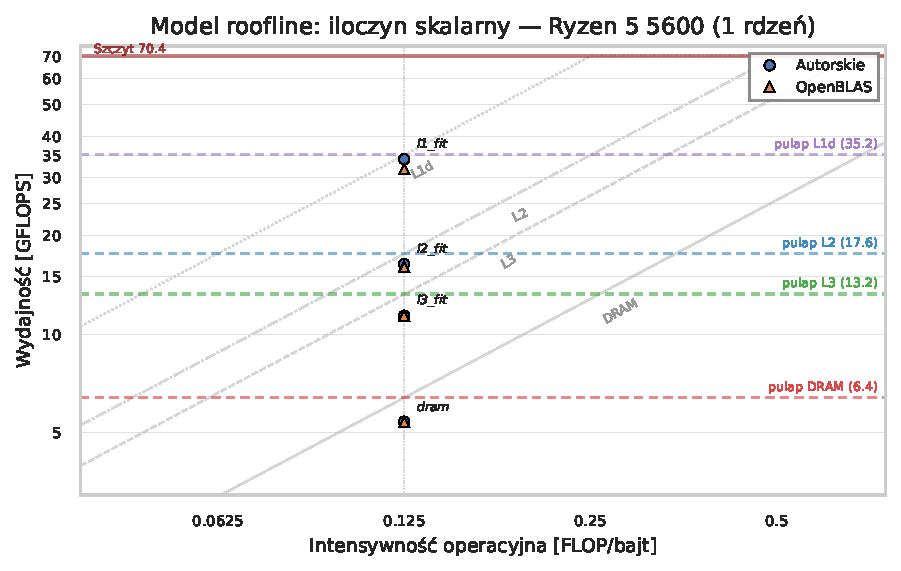
\includegraphics[width=0.72\textwidth]{roofline_dot}
\caption{Model roofline dla iloczynu skalarnego (tryb jednowątkowy): punkty pomiarowe najlepszego wariantu autorskiego oraz biblioteki OpenBLAS dla czterech presetów, naniesione przy stałej intensywności operacyjnej $0{,}125$ działania na bajt na tle skośnych pułapów przepustowości kolejnych poziomów pamięci oraz poziomego pułapu szczytowej mocy obliczeniowej. Wariant autorski trafia w pułap przepustowości poziomu, w którym mieści się zbiór roboczy}
\label{rys:roofline-dot}
\end{figure}

Najwyraźniej zachowanie operacji ograniczonej przepustowością ujawnia się dla danych w pamięci operacyjnej (preset \texttt{dram}). Wszystkie zwektoryzowane warianty (niezależnie od liczby akumulatorów) zbiegają do około 5,4 GFLOPS, czyli do wartości wyznaczonej przez zmierzoną w podrozdziale \ref{sec:srodowisko} osiągalną przepustowość odczytu z pamięci operacyjnej (około 42 GB/s, co przy tej intensywności daje $42 \cdot 0{,}125 \approx 5{,}3$ GFLOPS). Skośną prostą poziomu DRAM na rysunku \ref{rys:roofline-dot} wykreślono dla teoretycznego pułapu przepustowości modułów (51,2 GB/s), wobec czego punkty pamięci operacyjnej leżą wyraźnie poniżej niej (5,4 wobec 6,4 GFLOPS) --- zgodnie ze zmierzoną na maszynie osiągalną przepustowością odczytu (42 GB/s), niższą od nominalnej. Przewaga wariantu ośmioakumulatorowego, rozstrzygająca w pamięci podręcznej, tu całkowicie zanika: technika wielu łańcuchów ukrywa opóźnienie jednostek obliczeniowych, lecz nie zwiększa przepustowości pamięci, która jest tu czynnikiem wiążącym. Jedynie naiwna pętla skalarna pozostaje wolniejsza (2,8 GFLOPS), pozbawiona wektoryzacji, jest ograniczona opóźnieniem własnego łańcucha zależności. Zbieżność wszystkich szybkich wariantów do wspólnego pułapu na każdym poziomie pamięci jest istotą zachowania operacji ograniczonej przepustowością; ilustruje ją rysunek \ref{rys:size-dot}, na którym wydajność najlepszego wariantu opada schodkowo wraz ze wzrostem zbioru roboczego, za każdym razem gdy przekracza on pojemność kolejnego poziomu pamięci podręcznej.

\begin{figure}[t!]
\centering
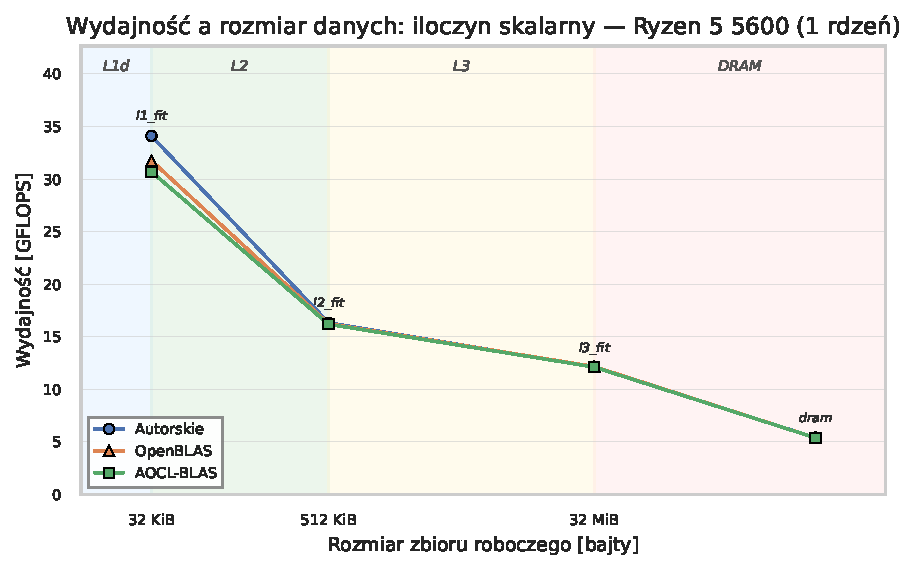
\includegraphics[width=0.72\textwidth]{size_dot}
\caption{Iloczyn skalarny: wydajność najlepszego wariantu autorskiego oraz biblioteki OpenBLAS w funkcji rozmiaru zbioru roboczego (tryb jednowątkowy). Pionowe pasy odpowiadają pojemnościom kolejnych poziomów pamięci; wydajność opada schodkowo przy każdym przekroczeniu pojemności poziomu pamięci podręcznej}
\label{rys:size-dot}
\end{figure}

Tryb sześciowątkowy (kolumny 6T w tabeli \ref{tab:wyniki-dot}; rysunek \ref{rys:dot-slupki}) potwierdza wnioski płynące z modelu roofline od drugiej strony. Zrównoleglenie przynosi zysk wyłącznie tam, gdzie wraz z liczbą rdzeni rośnie dostępne sumaryczne pasmo pamięci podręcznej. W presetach \texttt{l2\_fit} oraz \texttt{l3\_fit} wariant OpenMP skacze z około 12--14 GFLOPS jednowątkowo do około 44 GFLOPS --- każdy rdzeń dysponuje bowiem własną pamięcią podręczną L2, a współdzielona L3 oferuje sumarycznie znacznie wyższe pasmo niż widziane przez pojedynczy rdzeń. Natomiast w presecie \texttt{l1\_fit} (dane i tak prywatne dla rdzenia) oraz \texttt{dram} (wspólne, nasycone już przez jeden rdzeń pasmo pamięci operacyjnej) zrównoleglenie nie pomaga; w pamięci operacyjnej wynik jest wręcz nieco gorszy (4,7 GFLOPS), gdyż do nasyconego pasma dochodzi narzut koordynacji wątków. Biblioteki referencyjne zachowują się analogicznie, osiągając w L2 i L3 około 39--44 GFLOPS. Wniosek z modelu roofline jest zatem dwojaki: zrównoleglenie podnosi osiągalny pułap wyłącznie wtedy, gdy operacja korzysta z sumarycznego pasma pamięci podręcznej, a nie ze wspólnego, nasycalnego pasma pamięci operacyjnej.

\begin{figure}[t!]
\centering
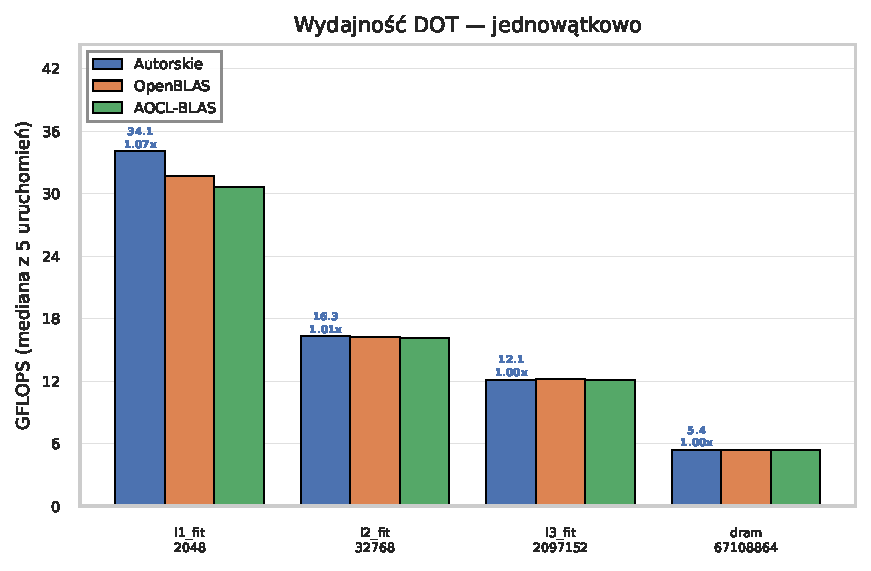
\includegraphics[width=0.86\textwidth]{dot_1t}\\[6pt]
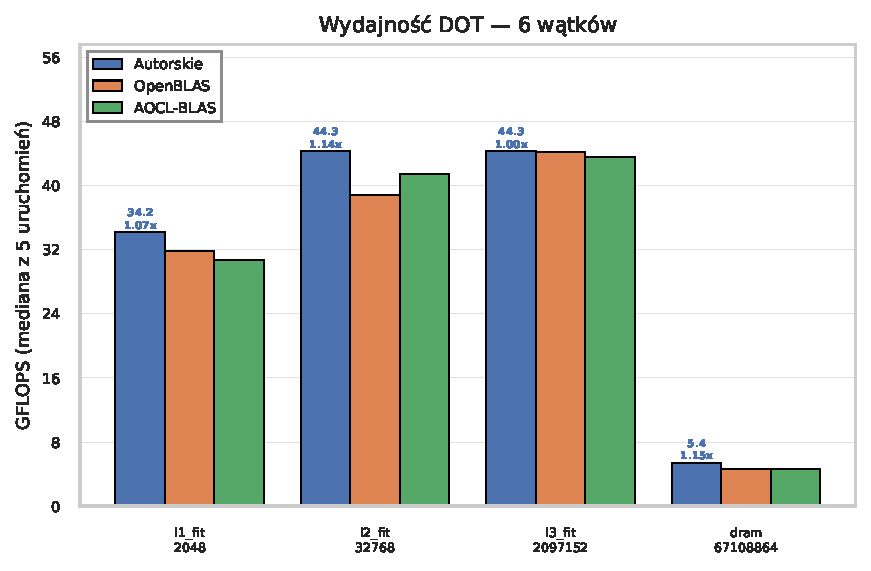
\includegraphics[width=0.86\textwidth]{dot_6t}
\caption{Iloczyn skalarny: najlepszy wariant autorski na tle bibliotek referencyjnych w czterech presetach --- u góry tryb jednowątkowy (1T), u dołu sześciowątkowy (6T). Liczby nad słupkami autorskimi podają wydajność oraz przyspieszenie względem OpenBLAS}
\label{rys:dot-slupki}
\end{figure}

\section{Mnożenie macierzy przez wektor}
\label{sec:wyniki-gemv}

Mnożenie macierzy przez wektor jest (podobnie jak iloczyn skalarny) operacją ograniczoną przepustowością pamięci. Jej intensywność operacyjną wyznaczono w podrozdziale \ref{sec:op-gemv}: wynosi ona 0,25 działania na bajt i jest w praktyce stała, gdyż każdy element macierzy $A$ odczytywany jest dokładnie raz. Wyniki dla sześciu presetów (tabela \ref{tab:gemv-presety}) zestawiono w tabeli \ref{tab:wyniki-gemv}, a położenie najlepszego wariantu względem pułapów roofline przedstawia rysunek \ref{rys:roofline-gemv} (dla czytelności pominięto na nim presety \texttt{wide} i \texttt{tall}, o niemal tej samej intensywności co \texttt{medium} i \texttt{large}).

\begin{table}[t!]
\centering
\caption{Mnożenie macierzy przez wektor --- wydajność (GFLOPS, mediana z maksymalnie pięciu przebiegów --- dla najdłuższych wywołań liczbę przebiegów protokół redukuje do dwóch lub jednego) w trybie jednowątkowym (1T) i sześciowątkowym (6T) dla sześciu presetów (tabela \ref{tab:gemv-presety}). Techniki kolejnych wariantów opisano w tabeli \ref{tab:gemv-impl}}
\label{tab:wyniki-gemv}
{\footnotesize
\setlength{\tabcolsep}{3pt}
\begin{tabular}{p{2.7cm} rr rr rr rr rr rr}
\hline
 & \multicolumn{2}{c}{\texttt{tiny}} & \multicolumn{2}{c}{\texttt{small}} & \multicolumn{2}{c}{\texttt{medium}} & \multicolumn{2}{c}{\texttt{large}} & \multicolumn{2}{c}{\texttt{wide}} & \multicolumn{2}{c}{\texttt{tall}} \\
Implementacja & 1T & 6T & 1T & 6T & 1T & 6T & 1T & 6T & 1T & 6T & 1T & 6T \\
\hline
naiwna (skalarna)            &  5,0 &  5,0 &  3,7 &  3,7 &  3,1 &   3,1 &  2,8 &  2,8 &  3,0 &   3,0 &  3,7 &   3,7 \\
wektoryzacja AVX2            & 28,3 & 28,3 & 23,0 & 22,4 & 19,9 &  19,7 & 10,1 & 10,0 & 16,0 &  16,5 & 22,5 &  22,5 \\
{}+ prefetch programowy      & 26,9 & 27,0 & 21,9 & 22,0 & 19,5 &  19,4 & 10,3 & 10,3 & 15,5 &  16,0 & 22,3 &  22,3 \\
jądro FMA, blok. 4-wierszowe & 38,0 & 37,8 & 25,0 & 24,5 & 23,0 &  22,9 & 13,1 & 12,7 & 22,9 &  23,2 & 22,6 &  22,9 \\
{}+ podwójne akumulatory     & 41,6 & 41,1 & 26,0 & 26,4 & 23,2 &  23,1 & 13,1 & 13,0 & 23,3 &  23,6 & 23,7 &  23,5 \\
{}+ blokowanie cache         & 35,8 & 35,5 & 25,2 & 24,5 & 19,2 &  20,2 &  8,5 &  8,2 & 15,6 &  16,4 & 22,4 &  22,8 \\
zrównoleglenie OpenMP        & 40,4 & 40,1 & 23,0 & 80,9 & 22,8 & 101,3 & 13,1 & 12,7 & 22,7 & 104,3 & 23,3 & 103,8 \\
OpenBLAS                     & 29,6 & 30,3 & 23,2 & 24,0 & 22,8 & 100,7 & 11,7 &  8,9 & 23,2 &  92,5 & 21,9 &  98,8 \\
AOCL-BLAS                    & 33,0 & 34,5 & 21,2 & 75,5 & 23,9 & 103,9 & 12,4 &  7,6 & 17,8 &  75,1 & 23,1 & 104,2 \\
\hline
\end{tabular}
}
\end{table}

W trybie jednowątkowym, dla najmniejszej macierzy mieszczącej się w pamięci podręcznej L1d (preset \texttt{tiny}), kolejne warianty ponownie tworzą drabinę wydajności: od naiwnej pętli skalarnej (5,0 GFLOPS), przez wektoryzację AVX2 (28,3 GFLOPS), aż po jądro FMA przetwarzające cztery wiersze naraz z reużyciem wektora $\mathbf{x}$ (38,0 GFLOPS) oraz jego wariant z podwójnymi akumulatorami, dający osiem niezależnych łańcuchów FMA --- 41,6 GFLOPS. Jawny prefetch programowy nie przynosi tu poprawy (26,9 GFLOPS), gdyż dane i tak rezydują już w pamięci podręcznej. Co istotne, mimo niewielkiego rozmiaru macierzy najlepszy wariant autorski przewyższa obie biblioteki referencyjne (OpenBLAS 29,6, AOCL-BLAS 33,0 GFLOPS): dla małych zadań w wyniku bibliotek znaczący udział ma stały narzut wywołania procedury. Osiągniętych 41,6 GFLOPS pozostaje przy tym wyraźnie poniżej pułapu przepustowości L1d dla tej intensywności ($281{,}6 \cdot 0{,}25 \approx 70{,}4$ GFLOPS) --- przy krótkich, 64-elementowych wierszach wiążącym ograniczeniem nie jest pasmo pamięci, lecz narzut redukcji poziomych i pętli resztkowych przypadający na każdy wiersz (rysunek \ref{rys:roofline-gemv}).

\begin{figure}[t!]
\centering
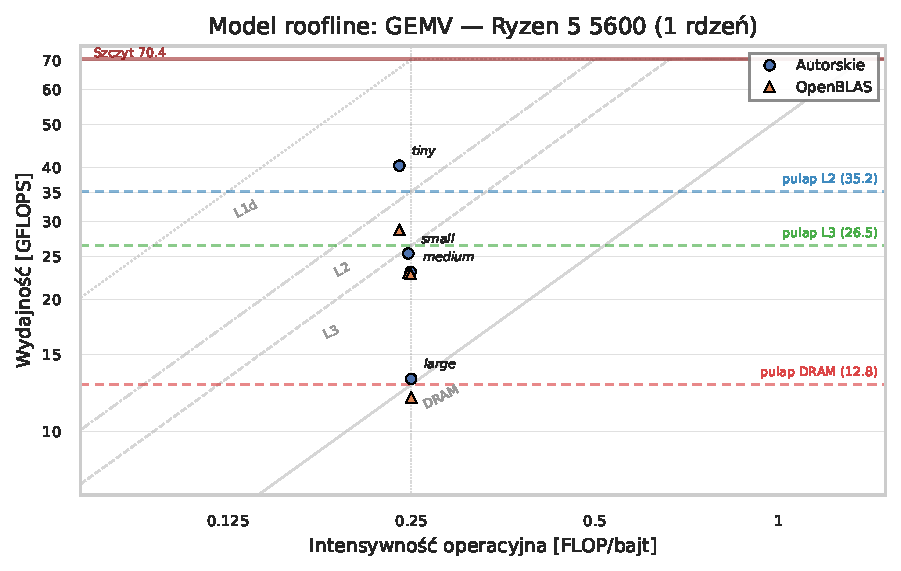
\includegraphics[width=0.72\textwidth]{roofline_gemv}
\caption{Model roofline dla mnożenia macierzy przez wektor (tryb jednowątkowy) przy intensywności operacyjnej $0{,}25$ działania na bajt. Punkt presetu \texttt{large} (macierz w pamięci operacyjnej) leży przy skośnym pułapie przepustowości DRAM, nieznacznie go przekraczając wskutek częściowej rezydencji macierzy w pamięci L3 między iteracjami pętli pomiarowej; punkt \texttt{tiny} pozostaje poniżej pułapu L1d, ograniczony narzutem obliczeń przy krótkich wierszach, a nie przepustowością pamięci}
\label{rys:roofline-gemv}
\end{figure}

W miarę wzrostu macierzy wydajność najlepszego wariantu opada wraz z przechodzeniem do coraz wolniejszych poziomów pamięci (rysunek \ref{rys:size-gemv}): w presecie \texttt{medium} (macierz w pamięci podręcznej L3) wariant z podwójnymi akumulatorami osiąga 23,2 GFLOPS, czyli około 87\% pułapu L3 dla tej intensywności ($106 \cdot 0{,}25 \approx 26{,}5$ GFLOPS). Decydujący jest jednak preset \texttt{large}, w którym macierz o objętości 128 MiB rezyduje w pamięci operacyjnej: warianty z reużyciem wektora $\mathbf{x}$ osiągają tu 13,1 GFLOPS. Wartość ta odpowiada ruchowi danych około $52{,}4$ GB/s, a więc nieznacznie przekracza zarówno teoretyczny pułap modułów DDR4-3200 ($51{,}2 \cdot 0{,}25 \approx 12{,}8$ GFLOPS), jak i --- wyraźniej --- przepustowość zmierzoną na maszynie ($42$ GB/s, czyli $\approx 10{,}5$ GFLOPS przy tej intensywności). Czysto strumieniowy odczyt z pamięci operacyjnej nie mógłby pułapu przekroczyć; najpewniejszym wyjaśnieniem jest częściowa rezydencja macierzy w pamięci podręcznej L3 między iteracjami pętli pomiarowej: 32 MiB pamięci L3 mieści około jednej czwartej 128-megabajtowej macierzy, co obniża rzeczywisty ruch z pamięci operacyjnej (przy 25\% reużycia wymagane pasmo spada do $\approx 39{,}3$ GB/s, poniżej zmierzonych 42 GB/s, i rachunek się domyka). Operacja pozostaje więc ograniczona przepustowością, lecz odniesienie do samego teoretycznego pułapu DRAM jest tu zaniżone o efekt pamięci podręcznej. Również w tym presecie autorskie warianty przewyższają biblioteki (OpenBLAS 11,7, AOCL-BLAS 12,4 GFLOPS).

\begin{figure}[t!]
\centering
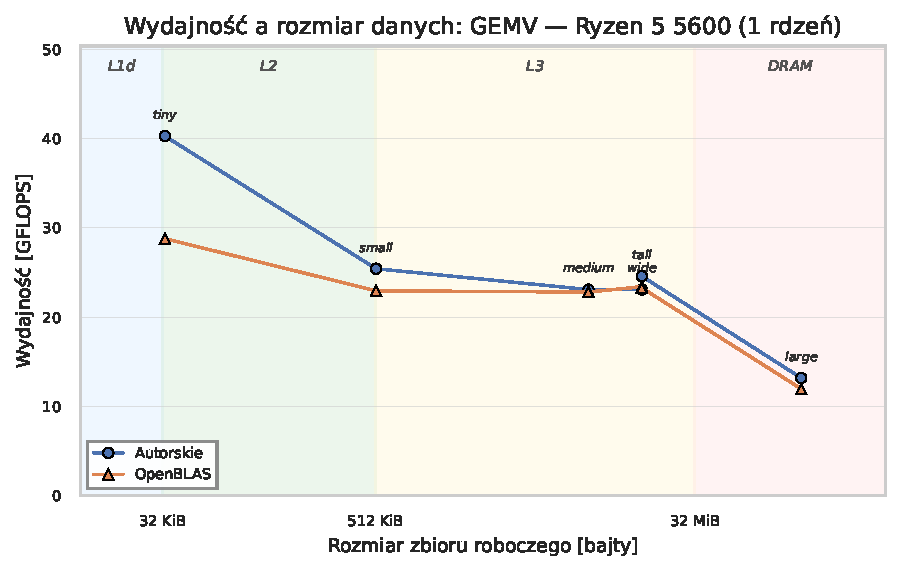
\includegraphics[width=0.72\textwidth]{size_gemv}
\caption{Mnożenie macierzy przez wektor: wydajność najlepszego wariantu autorskiego oraz biblioteki OpenBLAS w funkcji rozmiaru zbioru roboczego (tryb jednowątkowy); pionowe pasy odpowiadają pojemnościom kolejnych poziomów pamięci}
\label{rys:size-gemv}
\end{figure}

Preset \texttt{large} ujawnia zarazem granicę użyteczności blokowania pamięci podręcznej dla tej operacji. Wariant z jawnym kafelkowaniem wierszy i kolumn osiąga w nim jedynie 8,5 GFLOPS --- wyraźnie mniej niż prostsze warianty z reużyciem wektora $\mathbf{x}$ (13,1 GFLOPS). Powody są dwa i wynikają ze specyfiki operacji: po pierwsze, macierz $A$ jest i tak odczytywana tylko raz, więc blokowanie nie zmniejsza dominującego strumienia danych, a jedynie poprawia lokalność wektora $\mathbf{x}$, którego udział w ruchu pamięci jest znikomy; po drugie, jądro kafelkujące prowadzi obliczenia z jednym akumulatorem na wiersz (cztery łańcuchy FMA zamiast ośmiu), co obniża równoległość obliczeń. Presety o niesymetrycznym kształcie (\texttt{wide}, \texttt{tall}) potwierdzają, że zysk z reużycia wektora $\mathbf{x}$ zależy od proporcji macierzy: w obu wariant z reużyciem osiąga około 23--24 GFLOPS, czyli wydajność typową dla poziomu L3.

Tryb sześciowątkowy (kolumny 6T w tabeli \ref{tab:wyniki-gemv}; rysunek \ref{rys:gemv-slupki}) ponownie potwierdza wnioski roofline, wymaga jednak uwzględnienia warunkowego progu zrównoleglenia opisanego w podrozdziale \ref{sec:impl-gemv}. Zrównoleglony wariant autorski skaluje się wyraźnie tam, gdzie macierz mieści się w pamięci podręcznej L3 i dostępne jest sumaryczne pasmo wielu rdzeni: w presecie \texttt{medium} przechodzi z 22,8 do 101,3 GFLOPS, a w presetach \texttt{wide} i \texttt{tall} --- do około 104 GFLOPS. Inaczej zachowują się presety skrajne. Dla najmniejszej macierzy (\texttt{tiny}, poniżej dolnego progu) oraz dla największej (\texttt{large}, powyżej progu górnego) wariant ten z założenia wraca do ścieżki sekwencyjnej: nie tworzy wówczas regionu równoległego, więc jego wynik 6T (odpowiednio 40,1 i 12,7 GFLOPS) jest w istocie powtórzonym pomiarem jądra jednowątkowego, a nie skutkiem zrównoleglenia. Dla presetu \texttt{large} oznacza to, że wariant świadomie unika degradacji, która dotyka biblioteki: te rzeczywiście zrównoleglają ograniczoną pasmem pamięci operacyjnej operację i tracą na wydajności względem trybu jednowątkowego (OpenBLAS spada do 8,9, AOCL-BLAS do 7,6 GFLOPS). Tezę o nasyceniu wspólnego pasma pamięci operacyjnej już przez pojedynczy rdzeń potwierdza natomiast (bezpośrednim pomiarem) bezwarunkowo zrównoleglany wariant iloczynu skalarnego, który w presecie \texttt{dram} faktycznie spada z 5,4 do 4,7 GFLOPS (podrozdział \ref{sec:wyniki-dot}).

\begin{figure}[t!]
\centering
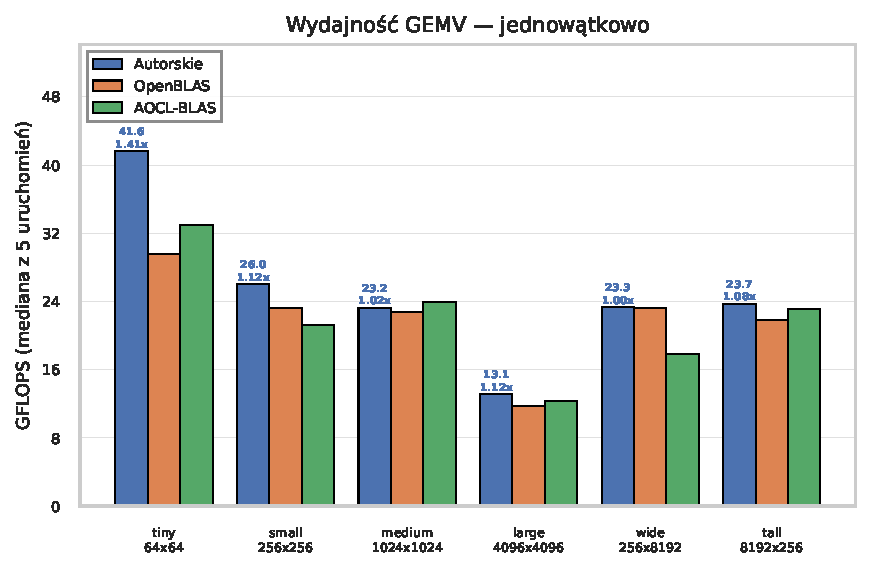
\includegraphics[width=0.86\textwidth]{gemv_1t}\\[6pt]
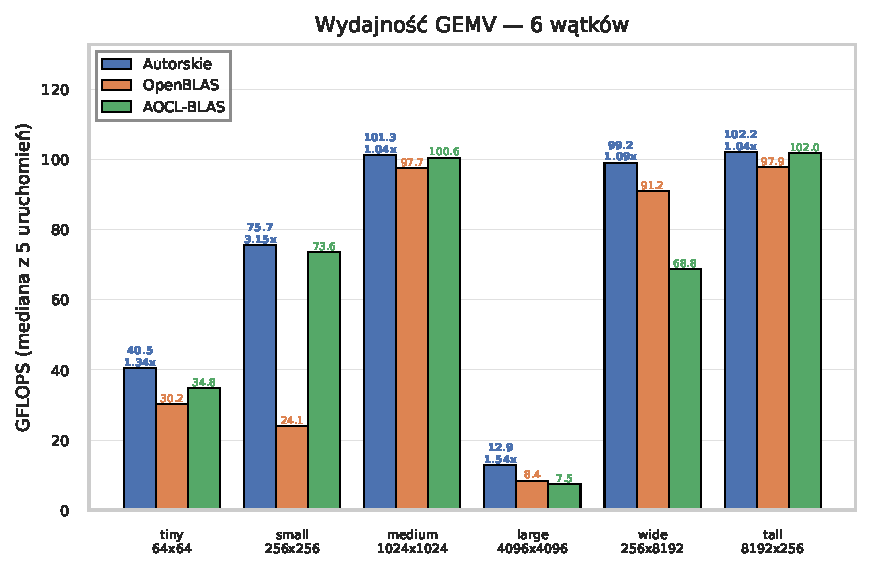
\includegraphics[width=0.86\textwidth]{gemv_6t}
\caption{Mnożenie macierzy przez wektor: najlepszy wariant autorski na tle bibliotek referencyjnych w sześciu presetach --- u góry tryb jednowątkowy (1T), u dołu sześciowątkowy (6T). Liczby nad słupkami autorskimi podają wydajność oraz przyspieszenie względem OpenBLAS}
\label{rys:gemv-slupki}
\end{figure}

\section{Mnożenie dwóch macierzy}
\label{sec:wyniki-gemm}

Mnożenie dwóch macierzy jest operacją poziomu trzeciego BLAS, której intensywność operacyjna rośnie wraz z rozmiarem macierzy (podrozdziały \ref{sec:op-gemm} i \ref{sec:impl-gemm}). Jest to więc operacja ograniczona mocą obliczeniową, a nie przepustowością pamięci: przy odpowiedniej organizacji obliczeń decyduje o niej utrzymanie jednostek FMA w ciągłej pracy, a osiągalnym pułapem jest szczytowa moc obliczeniowa procesora (około 70 GFLOPS dla liczb podwójnej precyzji, podrozdział \ref{sec:avx}). Z tego względu wyników nie analizuje się tu w odniesieniu do modelu roofline: ponieważ intensywność rośnie z rozmiarem, punkty pomiarowe leżałyby tuż pod poziomym pułapem szczytowym niezależnie od rozmiaru danych, a wykres roofline nie wnosiłby informacji. Analizę prowadzi się zamiast tego wzdłuż drabiny kolejnych optymalizacji, w odniesieniu do pułapu szczytowego (krzywa zależności wydajności od rozmiaru, rysunek \ref{rys:size-gemm}) oraz do wydajności bibliotek referencyjnych. Pełne wyniki dla siedmiu presetów (tabela \ref{tab:gemm-presety}) zestawiono w tabeli \ref{tab:wyniki-gemm}.

\begin{landscape}
\begin{table}
\centering
\caption{Mnożenie dwóch macierzy --- wydajność (GFLOPS, mediana z maksymalnie pięciu przebiegów --- dla najdłuższych wywołań liczbę przebiegów protokół redukuje do dwóch lub jednego) w trybie jednowątkowym (1T) i sześciowątkowym (6T) dla siedmiu presetów (tabela \ref{tab:gemm-presety}). Techniki kolejnych wariantów opisano w tabeli \ref{tab:gemm-impl}; ,,---'' oznacza pomiar pominięty (limit czasu)}
\label{tab:wyniki-gemm}
\footnotesize
\setlength{\tabcolsep}{4.5pt}
\begin{tabular}{l rr rr rr rr rr rr rr}
\hline
 & \multicolumn{2}{c}{\texttt{tiny}} & \multicolumn{2}{c}{\texttt{small}} & \multicolumn{2}{c}{\texttt{medium}} & \multicolumn{2}{c}{\texttt{large}} & \multicolumn{2}{c}{\texttt{rank\_k}} & \multicolumn{2}{c}{\texttt{tall\_K}} & \multicolumn{2}{c}{\texttt{odd}} \\
Implementacja & 1T & 6T & 1T & 6T & 1T & 6T & 1T & 6T & 1T & 6T & 1T & 6T & 1T & 6T \\
\hline
naiwna ($i$-$j$-$k$)                     &  4,6 &   4,6 &  1,3 &   1,3 &  0,4 &   0,4 &  --- &   --- &  0,9 &   0,9 &  0,2 &   0,2 &  3,3 &   3,3 \\
kolejność $i$-$k$-$j$                    & 20,9 &  20,9 & 20,5 &  20,0 & 20,1 &  19,4 &  9,8 &   9,8 & 18,4 &  18,5 & 13,3 &  13,3 & 18,4 &  18,5 \\
{}+ blokowanie pamięci podręcznej        & 20,1 &  20,3 & 22,4 &  22,4 & 14,8 &  14,9 & 11,7 &  11,7 & 21,5 &  21,0 & 14,4 &  14,7 & 21,7 &  21,3 \\
packing, mikrojądro $6 \times 8$         & 30,9 &  31,0 & 48,7 &  48,4 & 59,8 &  59,9 & 62,5 &  62,9 & 58,8 &  58,6 & 44,7 &  44,2 & 57,7 &  57,4 \\
mikrojądro $4 \times 12$ (asembler)      & 30,9 &  30,7 & 48,7 &  48,3 & 60,0 &  60,1 & 62,7 &  62,7 & 56,8 &  53,2 & 52,0 &  51,4 & 63,4 &  59,2 \\
mikrojądro $4 \times 12$ (funkcje wbud.) & 25,7 &  25,7 & 28,3 &  28,2 & 29,2 &  29,2 & 29,3 &  29,3 & 28,2 &  28,3 & 27,1 &  27,1 & 29,7 &  29,2 \\
ścieżka małych macierzy                  & 31,9 &  31,7 & 29,7 &  29,6 & 23,9 &  23,7 &  --- &   --- & 24,4 &  24,5 & 14,9 &  15,0 & 29,3 &  29,1 \\
równoległy, mikrojądro $6 \times 8$      & 30,2 &  56,5 & 48,6 & 148,2 & 59,8 & 226,5 & 62,5 & 111,2 & 58,7 & 204,2 & 44,7 &  86,4 & 57,6 & 183,5 \\
równoległy, osobny bufor $B$             & 30,1 &  91,3 & 48,7 & 191,6 & 60,0 & 245,9 & 62,7 &  94,3 & 53,7 & 191,1 & 52,0 & 100,7 & 60,3 & 209,1 \\
{}+ współdzielony bufor $B$              & 30,0 &  17,9 & 48,6 &  41,9 & 60,0 & 228,9 & 62,7 & 253,2 & 53,7 & 212,7 & 52,0 &  50,4 & 60,3 & 172,0 \\
dyspozytor wg rozmiaru                   & 31,8 &  91,5 & 49,6 & 189,1 & 60,6 & 267,3 & 62,1 & 257,3 & 54,2 & 217,6 & 50,9 & 100,5 & 60,8 & 181,2 \\
algorytm Strassena                       & 31,8 &  91,7 & 49,6 & 199,9 & 60,5 & 264,0 & 65,5 & 235,2 & 54,2 & 219,5 & 50,8 & 104,1 & 60,7 & 180,6 \\
OpenBLAS                                 & 47,7 &  47,0 & 59,4 & 219,0 & 61,5 & 292,7 & 60,4 & 297,4 & 51,7 & 251,7 & 54,9 & 212,0 & 61,5 & 315,1 \\
AOCL-BLAS                                & 61,0 & 162,5 & 63,7 & 282,8 & 65,3 & 341,6 & 61,6 & 318,2 & 60,5 & 306,2 & 56,0 & 258,8 & 64,7 & 336,5 \\
\hline
\end{tabular}
\end{table}
\end{landscape}

W trybie jednowątkowym kolejne warianty pokazują, jak ważna dla tej operacji jest organizacja obliczeń. Naiwna potrójna pętla w kolejności $i$--$j$--$k$ osiąga dla macierzy $1024^3$ (preset \texttt{medium}) zaledwie 0,4 GFLOPS --- jej najbardziej wewnętrzna pętla przebiega macierz $B$ kolumnowo, z krokiem równym liczbie kolumn, co jest wzorcem skrajnie wrogim pamięci podręcznej i niepodatnym na wektoryzację. Sama zmiana kolejności pętli na $i$--$k$--$j$, przywracająca ciągły dostęp w pętli wewnętrznej, podnosi wynik do 20,1 GFLOPS, a dodanie blokowania pamięci podręcznej utrzymuje go na poziomie kilkunastu--dwudziestu kilku GFLOPS. Co warte odnotowania, samo blokowanie (bez pakowania) bywa wręcz szkodliwe: w presecie \texttt{medium} obniża wynik z 20,1 do 14,8 GFLOPS. Bez przepakowania danych do ciągłych buforów kafelkowanie wprowadza bowiem dodatkowe chybienia konfliktowe i nie usuwa nieciągłości dostępu wewnątrz kafla --- dopiero pakowanie (kolejny wariant) przynosi rozstrzygający zysk. Rozstrzygający jest dopiero czwarty wariant: pełna pięciopętlowa anatomia z packingiem i rejestrowym mikrojądrem $6 \times 8$ osiąga 59,8 GFLOPS --- skok blisko trzykrotny, który po raz pierwszy doprowadza operację w pobliże pułapu mocy obliczeniowej. Dostrojenie mikrojądra do kafelka $4 \times 12$, optymalnego dla Zen 3, daje wyniki na tym samym poziomie lub nieco wyższe (60,0 GFLOPS dla \texttt{medium}, 63,4 dla \texttt{odd}).

Najwyraźniejszym wynikiem tego podrozdziału jest zmierzony koszt wylewania rejestrów (ang. \emph{spilling}), zapowiedziany w podrozdziale \ref{sec:impl-gemm}. Wariant z mikrojądrem $4 \times 12$ zapisanym w czystych funkcjach wbudowanych osiąga jedynie około 29 GFLOPS i osiąga swój limit na tym poziomie niezależnie od rozmiaru macierzy (29,2 GFLOPS dla \texttt{medium}, 29,3 dla \texttt{large}), podczas gdy wariant z pętlą po $K$ zapisaną w asemblerze osiąga odpowiednio 60,0 oraz 62,7 GFLOPS --- ponad dwukrotnie więcej (2,06-- oraz 2,14-krotnie). Potwierdza to mechanizm omówiony w podrozdziale \ref{sec:impl-gemm}: kafelek $4 \times 12$ wykorzystuje wszystkie szesnaście architektonicznych rejestrów YMM, więc kompilator pozbawiony rejestru zapasowego odsyła część akumulatorów na stos, dokładając do każdej iteracji gorącej pętli dodatkowe odczyty i zapisy pamięci, co niweczy przewagę kafelka. Argument ten ma charakter architektoniczny, niezależny od wersji kompilatora --- stąd konieczność zapisania pętli wewnętrznej w asemblerze, którą realizują również biblioteki OpenBLAS i AOCL-BLAS (podrozdział \ref{sec:blas-implementacje}).


\begin{figure}[t!]
\centering
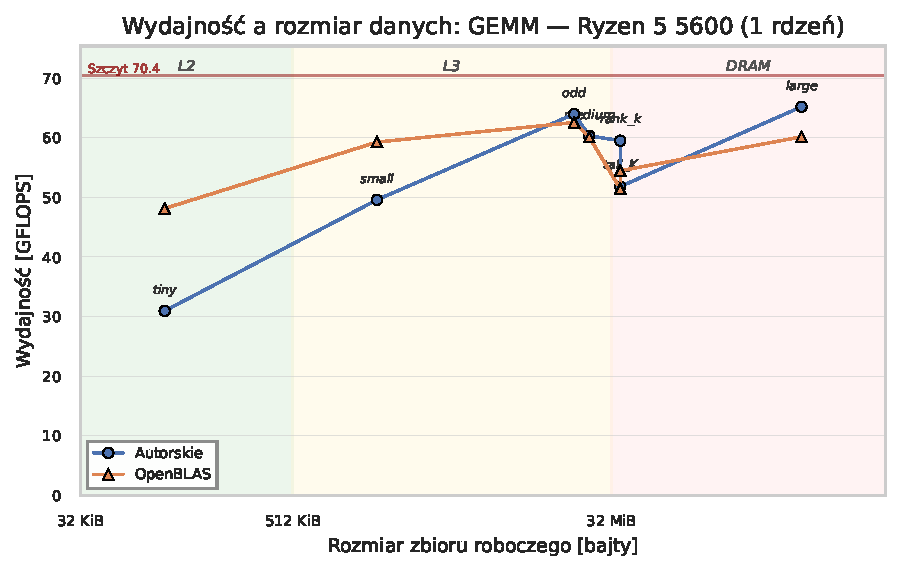
\includegraphics[width=0.72\textwidth]{size_gemm}
\caption{Mnożenie dwóch macierzy: wydajność najlepszego wariantu autorskiego oraz biblioteki OpenBLAS w funkcji rozmiaru zbioru roboczego (tryb jednowątkowy). Dzięki pakowaniu i blokowaniu wydajność utrzymuje się na plateau w pobliżu pułapu mocy obliczeniowej (około 85--89\% szczytu dla macierzy średnich i większych), mimo wzrostu zbioru roboczego i opuszczania kolejnych poziomów pamięci}
\label{rys:size-gemm}
\end{figure}

Utrzymanie wydajności mimo wzrostu rozmiaru macierzy jest wprost konsekwencją tego, że operacja jest ograniczona mocą obliczeniową: dzięki pakowaniu i blokowaniu najlepszy wariant utrzymuje szczyt możliwości na poziomie 60--63 GFLOPS (około 85--89\% pułapu szczytowego) od presetu \texttt{medium} aż po \texttt{large} (dla mniejszego presetu \texttt{small} jest to około 50 GFLOPS), podczas gdy wariant naiwny załamuje się wraz z opuszczeniem pamięci podręcznej (rysunek \ref{rys:size-gemm}). Kształt macierzy wpływa na to, który kafelek mikrojądra jest korzystniejszy: w presecie \texttt{tall\_K} (małe $M = 128$, duże $K$) kafelek $4 \times 12$ osiąga 52,0 GFLOPS wobec 44,7 dla kafelka $6 \times 8$ (węższy w wymiarze $M_R$ kafelek lepiej znosi małą liczbę wierszy), a w presecie \texttt{odd} o niewygodnych wymiarach wariant $4 \times 12$ sięga 63,4 GFLOPS, poprawnie obsługując brzegi. W porównaniu z bibliotekami najlepszy wariant autorski dorównuje w trybie jednowątkowym bibliotece OpenBLAS (48--62 GFLOPS) i ustępuje nieznacznie bibliotece AOCL-BLAS (56--65 GFLOPS), strojonej przez producenta procesora; wyjątkiem są najmniejsze macierze (\texttt{tiny}), w których obie biblioteki wyraźnie wygrywają (AOCL-BLAS 61,0 GFLOPS) dzięki dedykowanym ścieżkom dla małych zadań, oraz preset \texttt{rank\_k}, w którym najlepszy wariant autorski (58,8 GFLOPS, mikrojądro $6 \times 8$ z pakowaniem) przewyższa OpenBLAS (51,7 GFLOPS).

W trybie sześciowątkowym warianty równoległe skalują się do około 260--270 GFLOPS (dyspozytor osiąga 267,3 GFLOPS dla \texttt{medium}, 257,3 dla \texttt{large}), pozostając poniżej bibliotek, które skalują się lepiej (AOCL-BLAS do 341,6, OpenBLAS do 315,1 GFLOPS). Pomiary potwierdzają przy tym analizę z podrozdziału \ref{sec:impl-gemm} dotyczącą sposobu zarządzania buforem spakowanej macierzy $B$: żadna z dwóch strategii nie jest najlepsza we wszystkich przypadkach. Wariant z osobnym buforem $B$ dla każdego wątku nie jest wydajny dla największych macierzy (94,3 GFLOPS dla \texttt{large}), gdyż powielone kopie panelu $B$ wypierają się nawzajem ze współdzielonej pamięci podręcznej L3 --- to samo ograniczenie dotyka prostszego wariantu równoległego mikrojądra $6 \times 8$, opartego na tej samej strategii (111,2 GFLOPS dla \texttt{large}) --- sprawdza się natomiast dla zadań małych i średnich. Odwrotnie, wariant ze współdzielonym buforem $B$ utrzymuje wysoką wydajność dla dużych macierzy (253,2 GFLOPS dla \texttt{large}), lecz wykazuje niższą wydajność dla małych (17,9 GFLOPS dla \texttt{tiny}, 41,9 dla \texttt{small}), w których zrównoleglenie po grubych blokach $M_C$ daje zbyt mało pracy na wątek. Dyspozytor zależny od rozmiaru wybiera właściwą strategię dla danego kształtu zadania, łącząc zalety obu. Wariant Strassena, uruchamiany dopiero dla wymiarów parzystych i nie mniejszych niż próg $2048$ (a więc spośród badanych presetów wyłącznie dla \texttt{large}), osiąga wydajność zbliżoną do najlepszego wariantu gęstego. Porównanie najlepszego wariantu autorskiego z bibliotekami w obu trybach wątkowych przedstawia rysunek \ref{rys:gemm-slupki}.

\begin{figure}[t!]
\centering
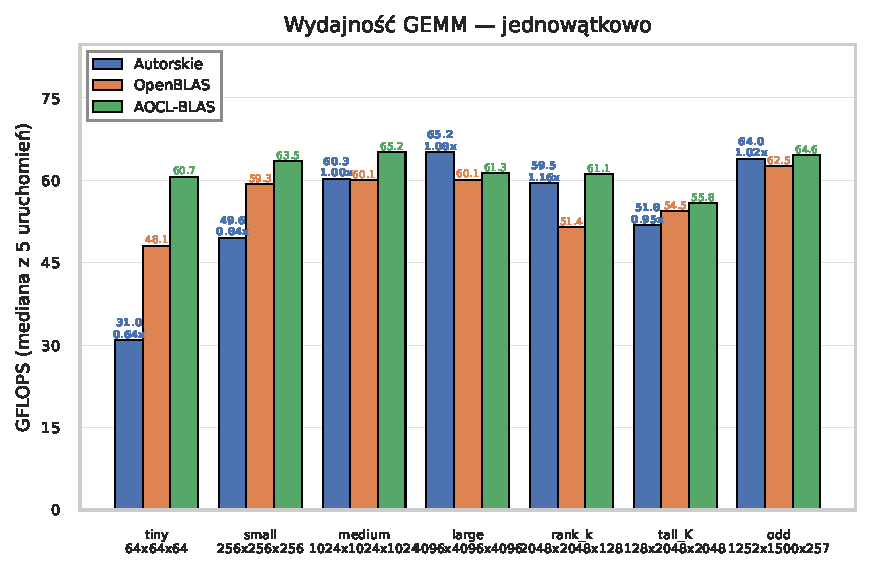
\includegraphics[width=0.86\textwidth]{gemm_1t}\\[6pt]
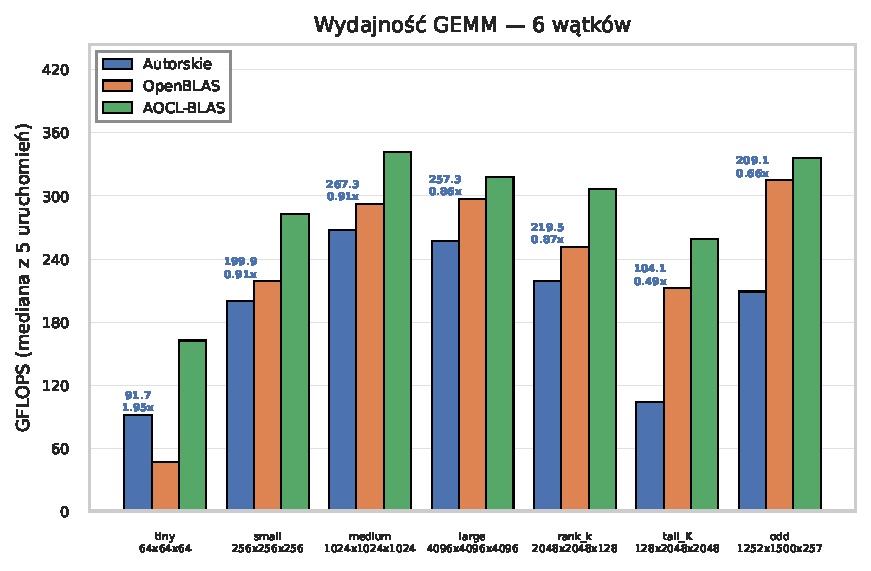
\includegraphics[width=0.86\textwidth]{gemm_6t}
\caption{Mnożenie dwóch macierzy: najlepszy wariant autorski na tle bibliotek referencyjnych w siedmiu presetach --- u góry tryb jednowątkowy (1T), u dołu sześciowątkowy (6T). Liczby nad słupkami autorskimi podają wydajność oraz przyspieszenie względem OpenBLAS}
\label{rys:gemm-slupki}
\end{figure}

\section{Splot dwuwymiarowy}
\label{sec:wyniki-conv}

Splot (podobnie jak mnożenie dwóch macierzy) ma wysoką intensywność operacyjną i jest operacją ograniczoną mocą obliczeniową (podrozdziały \ref{sec:splot-koszt} i \ref{sec:impl-conv}). Z tego względu, tak jak dla mnożenia macierzy, wyników nie analizuje się tu w odniesieniu do modelu roofline, lecz wzdłuż drabiny optymalizacji oraz względem pułapu szczytowego i wydajności bibliotek. Jedna różnica jest jednak istotna: splot zaimplementowano w pojedynczej precyzji (typ \texttt{float}), w której rejestr YMM mieści osiem wartości zamiast czterech, wobec czego szczytowa moc obliczeniowa jest dwukrotnie wyższa niż dla operacji podwójnej precyzji i wynosi około 141 GFLOPS (podrozdział \ref{sec:avx}, tabela \ref{tab:srodowisko}). Inaczej niż poprzednie operacje, splot nie ma pojedynczej najlepszej implementacji --- najwłaściwsza metoda zależy od kształtu warstwy, dlatego wariantem docelowym jest dyspozytor wybierający metodę na podstawie kształtu zadania (podrozdział \ref{sec:impl-conv}). Implementacje zmierzono dla dwunastu presetów (tabela \ref{tab:conv-presety}); wyniki dla kształtów standardowych z jądrem $3 \times 3$ oraz splotu punktowego zebrano w tabeli \ref{tab:wyniki-conv-a}, a dla większych jąder i obrazów RGB --- w tabeli \ref{tab:wyniki-conv-b}.

\begin{landscape}
\begin{table}
\centering
\caption{Splot --- wydajność (GFLOPS, mediana z maksymalnie pięciu przebiegów --- dla najdłuższych wywołań liczbę przebiegów protokół redukuje do dwóch lub jednego) w trybie jednowątkowym (1T) i sześciowątkowym (6T) dla presetów o jądrze $3 \times 3$ oraz splotu punktowego (tabela \ref{tab:conv-presety}). Techniki kolejnych wariantów opisano w tabeli \ref{tab:conv-impl}. W wierszach metod użytych poza ich domeną (np. Winograd dla presetu \texttt{pointwise}, splot $1 \times 1$ dla jąder $3 \times 3$) figuruje wynik ścieżki zastępczej, identyczny z wierszem mikrojądra bezpośredniego z pakowaniem}
\label{tab:wyniki-conv-a}
\footnotesize
\setlength{\tabcolsep}{4.5pt}
\begin{tabular}{l rr rr rr rr rr rr}
\hline
 & \multicolumn{2}{c}{\texttt{tiny}} & \multicolumn{2}{c}{\texttt{small}} & \multicolumn{2}{c}{\texttt{mid}} & \multicolumn{2}{c}{\texttt{large}} & \multicolumn{2}{c}{\texttt{xlarge}} & \multicolumn{2}{c}{\texttt{pointwise}} \\
Implementacja & 1T & 6T & 1T & 6T & 1T & 6T & 1T & 6T & 1T & 6T & 1T & 6T \\
\hline
naiwna (sześć pętli)               &  2,2 &   2,2 &   2,2 &   2,2 &   2,2 &   2,2 &   2,2 &   2,2 &   2,2 &   2,2 &   1,1 &   1,0 \\
zmiana kolejności pętli            & 17,4 &  17,1 &  24,7 &  24,7 &  16,9 &  17,0 &  10,3 &  10,2 &  10,3 &  10,3 &  28,9 &  31,7 \\
{}+ blokowanie pamięci podręcznej  & 19,6 &  19,2 &  25,0 &  24,9 &  16,9 &  17,0 &  10,2 &  10,2 &  10,2 &  10,2 &  31,9 &  31,5 \\
mikrojądro bezpośrednie, pakowanie &  3,7 &   3,7 &  11,7 &  11,7 &   5,4 &   5,4 &   2,2 &   2,2 &   2,2 &   2,2 &   6,4 &   6,4 \\
{}+ OpenMP                         &  3,7 &   8,9 &  11,7 &  34,5 &   5,3 &  28,2 &   2,2 &  11,1 &   2,2 &  11,4 &   6,4 &  34,8 \\
układ blokowy NCHWc8               & 84,2 & 268,2 &  94,4 & 502,5 &  76,1 & 422,2 &  89,2 & 442,3 &  86,4 & 451,6 &  63,7 & 321,9 \\
splot $1 \times 1$ jako SGEMM      &  3,7 &   3,7 &  11,7 &  11,7 &   5,4 &   5,3 &   2,2 &   2,2 &   2,2 &   2,2 & 112,6 & 569,1 \\
Winograd $F(2{,}3)$                & 63,6 &  82,0 & 145,1 & 567,5 & 123,2 & 527,0 &  44,6 & 231,4 &  48,4 & 261,8 &   6,4 &   6,4 \\
dyspozytor wg kształtu             & 84,1 & 267,7 & 145,1 & 570,0 & 123,4 & 537,1 &  89,2 & 476,5 &  86,4 & 450,9 & 112,8 & 529,4 \\
im2col $+$ OpenBLAS                & 73,4 &  92,0 & 112,3 & 403,8 & 117,2 & 444,6 & 118,6 & 427,3 & 121,8 & 485,5 & 108,0 & 477,0 \\
im2col $+$ AOCL-BLAS               & 87,8 & 107,1 & 111,6 & 425,7 & 112,6 & 449,8 & 127,1 & 560,8 & 127,6 & 571,5 & 123,6 & 513,7 \\
\hline
\end{tabular}
\end{table}
\end{landscape}

\begin{landscape}
\begin{table}
\centering
\caption{Splot --- wydajność (GFLOPS, mediana z maksymalnie pięciu przebiegów --- dla najdłuższych wywołań liczbę przebiegów protokół redukuje do dwóch lub jednego) w trybie jednowątkowym (1T) i sześciowątkowym (6T) dla presetów o większych jądrach ($5 \times 5$, $7 \times 7$) oraz obrazów RGB o trzech kanałach wejścia (tabela \ref{tab:conv-presety})}
\label{tab:wyniki-conv-b}
\footnotesize
\setlength{\tabcolsep}{4.5pt}
\begin{tabular}{l rr rr rr rr rr rr}
\hline
 & \multicolumn{2}{c}{\texttt{kernel5}} & \multicolumn{2}{c}{\texttt{kernel7}} & \multicolumn{2}{c}{\texttt{rgb3x3}} & \multicolumn{2}{c}{\texttt{rgb5x5}} & \multicolumn{2}{c}{\texttt{rgb7x7}} & \multicolumn{2}{c}{\texttt{rgb\_fhd}} \\
Implementacja & 1T & 6T & 1T & 6T & 1T & 6T & 1T & 6T & 1T & 6T & 1T & 6T \\
\hline
naiwna (sześć pętli)               &   2,8 &   2,7 &  2,6 &   2,6 &  2,6 &   2,6 &   3,1 &   3,1 &   2,8 &   2,8 &  2,6 &  2,6 \\
zmiana kolejności pętli            &  30,7 &  30,7 & 23,6 &  23,6 & 24,3 &  25,0 &  26,3 &  26,4 &  23,8 &  23,8 & 20,6 & 20,5 \\
{}+ blokowanie pamięci podręcznej  &  31,9 &  31,7 & 32,4 &  32,5 & 34,7 &  34,6 &  37,2 &  37,5 &  32,5 &  32,5 & 24,1 & 24,1 \\
mikrojądro bezpośrednie, pakowanie &  10,0 &  10,0 & 14,5 &  14,5 & 17,3 &  17,2 &  16,8 &  16,8 &  25,9 &  25,5 & 22,3 & 22,6 \\
{}+ OpenMP                         &  10,0 &  42,4 & 14,0 &  40,1 & 17,2 &  39,2 &  16,8 &  47,5 &  25,9 &  43,6 & 22,7 & 39,0 \\
układ blokowy NCHWc8               &  97,7 & 535,7 & 88,5 & 505,2 & 61,1 & 278,4 &  81,6 & 405,4 &  94,7 & 493,7 & 42,5 & 64,1 \\
splot $1 \times 1$ jako SGEMM      &  10,0 &  10,0 & 14,5 &  14,5 & 17,2 &  17,2 &  16,8 &  16,8 &  25,9 &  25,6 & 22,3 & 22,6 \\
Winograd $F(2{,}3)$                &  10,0 &  10,0 & 14,5 &  14,5 & 17,7 &  18,5 &  16,8 &  16,8 &  25,9 &  25,6 & 12,5 & 12,9 \\
dyspozytor wg kształtu             &  97,7 & 540,3 & 88,5 & 505,0 & 61,0 & 293,1 &  81,6 & 395,2 &  94,7 & 481,8 & 42,5 & 64,5 \\
im2col $+$ OpenBLAS                & 102,3 & 293,9 & 89,2 & 174,0 & 70,4 & 319,7 &  88,4 & 287,0 & 105,3 & 400,2 & 49,4 & 62,4 \\
im2col $+$ AOCL-BLAS               & 110,9 & 357,7 & 86,8 & 202,1 & 99,6 & 435,8 & 106,4 & 362,0 & 120,9 & 486,5 & 61,4 & 80,3 \\
\hline
\end{tabular}
\end{table}
\end{landscape}

W trybie jednowątkowym, dla typowej warstwy z jądrem $3 \times 3$, kolejne warianty ponownie tworzą drabinę wydajności. Naiwny splot sześciopętlowy osiąga około 2,2 GFLOPS, zmiana kolejności pętli i blokowanie pamięci podręcznej podnoszą wynik do kilkunastu--trzydziestu kilku GFLOPS, a mikrojądro bezpośrednie z pakowaniem (przeniesione wprost z mnożenia macierzy) okazuje się dla tej operacji rozczarowujące (od 2 do 26 GFLOPS). Przyczyną nie jest płytkość redukcji --- przeciwnie, najgorszy wynik dają presety \texttt{large} i \texttt{xlarge}, o najgłębszej spośród wszystkich presetów redukcji ($C_{\mathrm{in}} K_H K_W = 256 \cdot 9 = 2304$) --- lecz wymóg co najmniej szesnastu ciągłych pozycji wyjścia w wierszu, narzucony przez szerokość kafelka mikrojądra ($\mathrm{CONV\_NR} = 16$). Dla map węższych niż szesnaście kolumn, a takie mają presety \texttt{large} i \texttt{xlarge} ($O_W = 12$), oraz w resztkach wierszy obliczenie spada do skalarnej ścieżki brzegowej, równoważnej wariantowi naiwnemu; dla tych dwóch presetów cała praca wykonuje się tą ścieżką, stąd wynik na poziomie naiwnym (2,2 GFLOPS). Gradację pozostałych wyników wyjaśnia ułamek wiersza pokryty wektorowo: \texttt{small} ($O_W = 54$, czyli 48 z 54 kolumn) --- 11,7 GFLOPS, a \texttt{kernel7} ($O_W = 106$) --- 14,5 GFLOPS. Przełomem jest dopiero układ blokowy NCHWc8, w którym blok ośmiu kanałów wypełnia rejestr wektorowy: osiąga on od 76 do 94 GFLOPS, a więc po raz pierwszy doprowadza splot bezpośredni w pobliże wydajności charakterystycznej dla operacji ograniczonej mocą obliczeniową. Dla map cech o umiarkowanej liczbie kanałów najszybszy okazuje się jednak algorytm Winograda: w presetach \texttt{small} i \texttt{mid} osiąga on 145,1 oraz 123,2 GFLOPS. Pierwsza z tych wartości przekracza pułap szczytowy pojedynczej precyzji (około 141 GFLOPS), co nie jest sprzecznością: algorytm Winograda wykonuje, podobnie jak algorytm Strassena dla mnożenia macierzy (podrozdział \ref{sec:blas-strassen}), mniej działań arytmetycznych niż splot bezpośredni, względem którego liczona jest wydajność, więc wyrażona w ten sposób liczba ,,działań na sekundę'' może przewyższać fizyczny pułap jednostek FMA.

Żadna pojedyncza metoda nie jest jednak najlepsza dla wszystkich kształtów --- i to właśnie czyni dyspozytor wariantem docelowym. Jego skuteczność widać w tabeli \ref{tab:wyniki-conv-a}: dla każdego presetu osiąga on wydajność najlepszej metody dostępnej dla danego kształtu. Dla jądra $3 \times 3$ kieruje obliczenie na algorytm Winograda tam, gdzie jest on opłacalny, to jest gdy kafelków transformaty jest dostatecznie wiele, a kanałów dostatecznie dużo (\texttt{small}, \texttt{mid}: 145 i 123 GFLOPS), a w przeciwnym razie na układ blokowy NCHWc8, szybszy dla map małych lub o skrajnej liczbie kanałów (\texttt{tiny}, \texttt{large}, \texttt{xlarge}: 84, 89 i 86 GFLOPS), w których wsadowe mnożenia Winograda stają się zbyt chude. Progi tej decyzji (co najmniej $64$ kafelki oraz $\min(C_{\mathrm{in}}, C_{\mathrm{out}}) \ge 32$) dobrano empirycznie z krzywej skrzyżowania wydajności obu metod (podrozdział \ref{sec:impl-conv}). Splot punktowy $1 \times 1$ kierowany jest na ścieżkę czystego mnożenia macierzy (\texttt{pointwise}: 112,8 GFLOPS), a większe jądra $5 \times 5$ i $7 \times 7$ --- na układ blokowy NCHWc8 (97,7 i 88,5 GFLOPS).

Osobnym, wymagającym przypadkiem są obrazy wejściowe o trzech kanałach (format RGB), typowe dla pierwszej warstwy sieci. Obie najszybsze metody dla jądra $3 \times 3$ zawodzą tu z powodów strukturalnych: algorytm Winograda degeneruje się, gdyż wspólnym wymiarem jego mnożeń staje się sama liczba kanałów wejścia ($C_{\mathrm{in}} = 3$), dając skrajnie chude mnożenia i ogromne bufory pośrednie (szczególnie dla klatki Full HD), a układ blokowy NCHWc8 wymaga liczby kanałów będącej wielokrotnością ośmiu. Dlatego dla małej liczby kanałów wejścia dyspozytor kieruje obliczenie na mikrojądro bezpośrednie blokowane po kanałach wyjścia (podrozdział \ref{sec:impl-conv}). Wariant ten istotnie poprawia wydajność względem najlepszej z pozostałych metod bezpośrednich (blokowania pamięci podręcznej): dla presetu \texttt{rgb3x3} podnosi ją z 34,7 do 61,0 GFLOPS, dla \texttt{rgb5x5} z 37,2 do 81,6, dla \texttt{rgb7x7} z 32,5 do 94,7, a dla klatki Full HD (\texttt{rgb\_fhd}) z 24,1 do 42,5 GFLOPS, czyli od $1{,}7$ do $2{,}9$ razy.

W porównaniu z bibliotekami referencyjnymi, realizującymi splot przez rozwinięcie im2col i mnożenie macierzy (podrozdział \ref{sec:impl-conv}), obraz jest niejednoznaczny i zależy od kształtu warstwy. Dla map o umiarkowanej liczbie kanałów wariant autorski wygrywa lub dorównuje: w presecie \texttt{small} dyspozytor (algorytm Winograda) osiąga 145,1 GFLOPS wobec 111,6 dla im2col z AOCL-BLAS, a w presecie \texttt{kernel7} układ blokowy NCHWc8 (88,5 GFLOPS) dorównuje obu realizacjom bibliotecznym (89,2 i 86,8 GFLOPS), nie ponosząc przy tym narzutu pamięciowego rozwinięcia im2col, który przy jądrze $7 \times 7$ przekracza czterdziestokrotność rozmiaru wejścia. Uczciwie należy jednak odnotować przypadki przegrane. Dla małych map o bardzo wielu kanałach (\texttt{large}, \texttt{xlarge}) rozwinięcie im2col z biblioteką AOCL-BLAS (127,1 i 127,6 GFLOPS) przewyższa autorski układ blokowy NCHWc8 (89,2 i 86,4) --- niewielkie mapy sprzyjają tu sprowadzeniu splotu do pojedynczego, dużego mnożenia macierzy. Podobnie dla obrazów RGB chuda redukcja po trzech kanałach nadal faworyzuje pojedyncze duże mnożenie im2col (AOCL-BLAS osiąga 100--121 GFLOPS wobec autorskich 61--95), a dla klatki Full HD wynik autorski (42,5 GFLOPS) ustępuje bibliotece (61,4) z powodu dużych buforów pośrednich i wiążącej przepustowości pamięci.

W trybie sześciowątkowym szybkie jądra bezpośrednie skalują się bardzo dobrze: dla większości presetów o jądrze $3 \times 3$ i umiarkowanej liczbie kanałów układ blokowy NCHWc8 oraz algorytm Winograda osiągają od około 270 do 570 GFLOPS, a dyspozytor --- 570 GFLOPS dla \texttt{small}, 537 dla \texttt{mid}, 477 dla \texttt{large} oraz 505 dla \texttt{kernel7} (dla przypadków skrajnych, jak \texttt{tiny} czy obrazy RGB, wartości są wyraźnie niższe). W wielu przypadkach przewyższa to biblioteki, zwłaszcza dla dużych jąder (\texttt{kernel7}: 505,0 GFLOPS wobec 202,1 dla AOCL-BLAS). Wyjątkiem pozostają obrazy RGB, dla których zrównoleglone rozwinięcie im2col nadal bywa szybsze, oraz klatka Full HD, gdzie wynik autorski (64,5 GFLOPS) ogranicza przepustowość pamięci przy dużych buforach pośrednich. Porównanie najlepszego wariantu autorskiego (dyspozytora) z bibliotekami w obu trybach wątkowych przedstawia rysunek \ref{rys:conv-slupki}.

\begin{figure}[p]
\centering
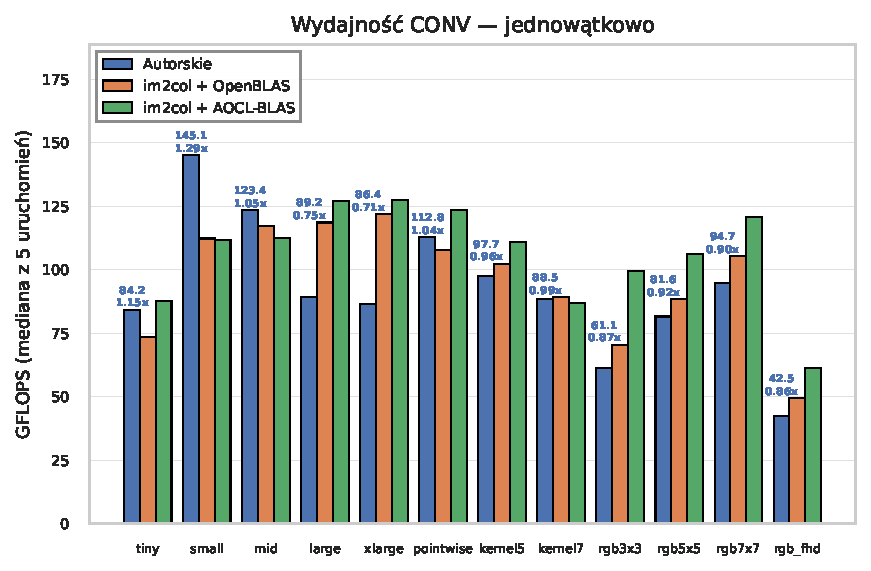
\includegraphics[width=\textwidth]{conv_1t}\\[8pt]
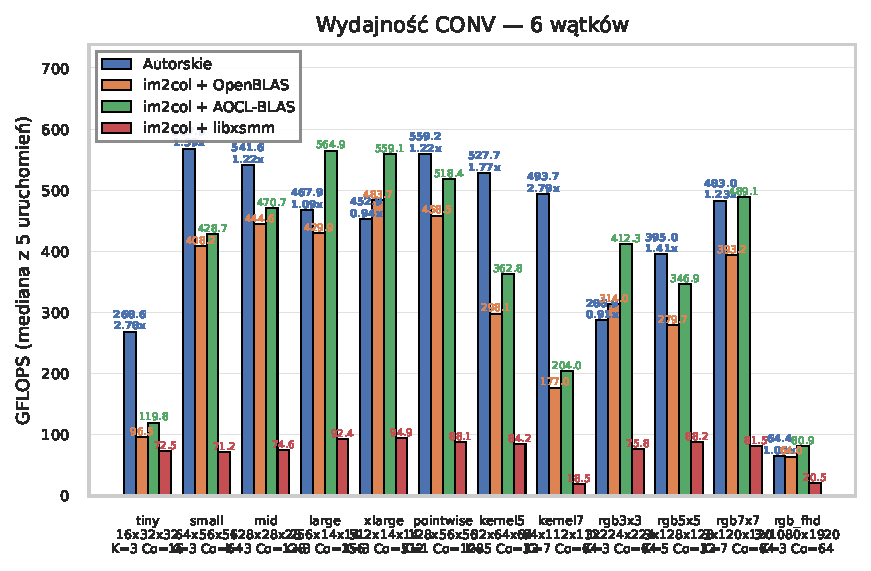
\includegraphics[width=\textwidth]{conv_6t}
\caption{Splot: najlepszy wariant autorski (dyspozytor) na tle bibliotek referencyjnych (im2col $+$ SGEMM) w dwunastu presetach --- u góry tryb jednowątkowy (1T), u dołu sześciowątkowy (6T). Liczby nad słupkami autorskimi podają wydajność oraz przyspieszenie względem im2col z OpenBLAS}
\label{rys:conv-slupki}
\end{figure}

\section{Synteza wyników}
\label{sec:wyniki-synteza}

Zebrane pomiary potwierdzają tezę przewodnią pracy: techniki lokalności danych i wykorzystania pamięci podręcznej, omówione w rozdziałach \ref{chap:hierarchia} i \ref{chap:lokalnosc}, przekładają się bezpośrednio na wydajność, lecz osiągalny pułap oraz właściwa technika optymalizacji zależą od intensywności operacyjnej operacji. Podział na operacje ograniczone przepustowością pamięci oraz ograniczone mocą obliczeniową, wprowadzony w rozdziale \ref{chap:blas} i przyjęty jako oś niniejszego rozdziału, okazał się trafnym kryterium porządkującym wyniki.

Dla operacji ograniczonych przepustowością pamięci (iloczynu skalarnego i mnożenia macierzy przez wektor) osiągalną wydajność wyznacza przepustowość tego poziomu pamięci, w którym mieści się zbiór roboczy, a najlepsze warianty autorskie osiągają niemal odpowiadający im skośny pułap modelu roofline (iloczyn skalarny w pamięci podręcznej L1d --- 34,1 GFLOPS wobec pułapu 35,2; mnożenie macierzy przez wektor dla danych w pamięci operacyjnej --- 13,1 GFLOPS na poziomie pułapu DRAM rzędu 12,8, z niewielkim przekroczeniem tłumaczonym częściową rezydencją macierzy w pamięci L3 między iteracjami pomiaru). Optymalizacja (wektoryzacja, wiele niezależnych akumulatorów, reużycie wektora wspólnego dla wielu wierszy, wyrównanie danych i prefetch) służy tu wyłącznie pełnemu wykorzystaniu dostępnej przepustowości, nie zaś zmniejszeniu liczby działań. Zrównoleglenie podnosi osiągalny pułap jedynie tam, gdzie wraz z liczbą rdzeni rośnie sumaryczne pasmo pamięci podręcznej (poziomy L2 i L3), a nie dla wspólnego, nasycalnego pasma pamięci operacyjnej.

Dla operacji ograniczonych mocą obliczeniową (mnożenia dwóch macierzy i splotu) decydujące okazuje się utrzymanie jednostek FMA w ciągłej pracy za pomocą blokowania i packingu. Techniki te doprowadzają wydajność jednowątkową do plateau w pobliżu pułapu szczytowego (mnożenie macierzy utrzymuje 60--63 GFLOPS, czyli około 85--89\% szczytu, dla macierzy średnich i większych niezależnie od poziomu pamięci) i pozwalają na dobre skalowanie wielordzeniowe. Kluczowym składnikiem jest rejestrowe mikrojądro, a zmierzony koszt wylewania rejestrów (ponaddwukrotny spadek wydajności wariantu z funkcji wbudowanych względem asemblerowego) dowodzi, że dla kafelka optymalnego pod mikroarchitekturę Zen 3 zapisanie gorącej pętli w asemblerze wstawianym jest koniecznością wynikającą z liczby rejestrów wektorowych, a nie kwestią doboru kompilatora. Do tego samego rozwiązania uciekają się dojrzałe biblioteki.

W zestawieniu z bibliotekami referencyjnymi autorskie implementacje wypadają konkurencyjnie, choć nierównomiernie. W mnożeniu macierzy dorównują w trybie jednowątkowym bibliotece OpenBLAS i ustępują nieznacznie strojonej przez producenta bibliotece AOCL-BLAS. W splocie obraz zależy od kształtu warstwy: warianty autorskie wygrywają lub dorównują dla map o umiarkowanej liczbie kanałów oraz dla dużych jąder (gdzie kosztowna materializacja macierzy im2col osłabia biblioteki), a ustępują dla małych map o bardzo wielu kanałach oraz obrazów RGB, w których sprowadzenie splotu do pojedynczego dużego mnożenia macierzy pozostaje korzystniejsze. Co istotne, dla splotu żadna pojedyncza metoda nie jest najlepsza dla wszystkich kształtów; to dyspozytor wybierający metodę na podstawie kształtu warstwy (łączący splot bezpośredni w układzie NCHWc8, algorytm Winograda, ścieżkę splotu punktowego oraz mikrojądro blokowane po kanałach wyjścia dla małej liczby kanałów wejścia) zapewnia najlepszy wynik w całym zakresie badanych warstw.

Podsumowując, na konkretnej architekturze AMD Zen 3 (Ryzen 5 5600) techniki lokalności danych rozwinięte w rozdziałach teoretycznych pozwoliły starannie dostrojonym jądrom zbliżyć się do sprzętowych pułapów (przepustowości pamięci dla operacji pierwszego i drugiego poziomu oraz mocy obliczeniowej dla operacji trzeciego poziomu i splotu) i stanąć do porównania z bibliotekami produkcyjnymi. Wyniki ujawniły zarazem granice tego podejścia: architektoniczną konieczność asemblera dla kafelka optymalnego oraz zależność najlepszej metody obliczania splotu od kształtu warstwy.

\chapter*{Podsumowanie} % jak we wstępie
\addcontentsline{toc}{chapter}{Podsumowanie}
\chaptermark{Podsumowanie}

Celem niniejszej pracy była optymalizacja lokalności danych i wykorzystania pamięci podręcznej w implementacjach wybranych funkcji BLAS oraz operacji splotu dwuwymiarowego, osadzona w realiach konkretnej architektury, procesora AMD Ryzen 5 5600 z mikroarchitekturą Zen 3. Cel ten zrealizowano. Część teoretyczna (rozdziały \ref{chap:hierarchia}--\ref{chap:splot}) usystematyzowała wiedzę niezbędną do świadomego strojenia jąder obliczeniowych: budowę i organizację hierarchii pamięci oraz jednostek wektorowych procesora docelowego, techniki poprawy lokalności danych (blokowanie, packing, prefetching, wektoryzację oraz dobór układu danych), a także podział BLAS na trzy poziomy wraz z pojęciem intensywności operacyjnej i przegląd metod obliczania splotu. Część praktyczna (rozdziały \ref{chap:implementacja} oraz \ref{chap:wyniki}) ukazała te zagadnienia w praktyce.

W części praktycznej zaimplementowano cztery operacje (iloczyn skalarny, mnożenie macierzy przez wektor, mnożenie dwóch macierzy oraz splot dwuwymiarowy), każdą w szeregu wariantów o narastającym stopniu optymalizacji, od wersji naiwnej po jądra dostrojone do mikroarchitektury Zen 3. Wszystkie zmierzono jednolitym protokołem, w trybie jednowątkowym i wielowątkowym, i porównano z dojrzałymi bibliotekami OpenBLAS oraz AOCL-BLAS. Zebrane wyniki, omówione szczegółowo w syntezie podrozdziału \ref{sec:wyniki-synteza}, pokazują, że starannie dostrojone jądra autorskie zbliżają się do sprzętowych pułapów wydajności (przepustowości pamięci dla operacji ograniczonych pamięciowo oraz mocy obliczeniowej dla operacji ograniczonych obliczeniowo) i stają, choć nierównomiernie, do porównania z bibliotekami produkcyjnymi.

W ramach pracy osiągnięto w szczególności:
\begin{itemize}
  \item usystematyzowanie wiedzy teoretycznej --- o hierarchii pamięci i jednostkach wektorowych procesora docelowego, o technikach poprawy lokalności danych (blokowanie, pakowanie, prefetching, wektoryzacja, dobór układu danych), o poziomach BLAS wraz z intensywnością operacyjną oraz o metodach obliczania splotu;
  \item autorskie implementacje czterech operacji (iloczynu skalarnego, mnożenia macierzy przez wektor, mnożenia dwóch macierzy i splotu dwuwymiarowego) w wariantach o narastającej optymalizacji, z dostrojonym pod Zen 3 mikrojądrem mnożenia macierzy zapisanym w asemblerze;
  \item dyspozytory dobierające metodę lub ścieżkę obliczeń do kształtu zadania (dla mnożenia macierzy i dla splotu) oraz jednolity, automatyczny protokół pomiarowy z porównaniem do bibliotek OpenBLAS i AOCL-BLAS;
  \item przeprowadzenie dogłębnej analizy wydajności --- w odniesieniu do modelu roofline i sprzętowych pułapów, wzdłuż drabin kolejnych optymalizacji oraz w porównaniu z bibliotekami referencyjnymi, w trybie jedno- i sześciowątkowym;
  \item wykazanie, że dostrojone jądra zbliżają się do sprzętowych pułapów wydajności i stają do porównania z bibliotekami produkcyjnymi.
\end{itemize}

Przedstawione wyniki wyznaczają naturalne kierunki dalszych prac. Pierwszym jest przeniesienie tej samej metodyki na nowsze rozszerzenia wektorowe i mikroarchitektury, których szersze oraz liczniejsze rejestry wymagają ponownego doboru wymiarów kafelka mikrojądra, lecz nie zmieniają samej zasady postępowania. Drugim --- rozszerzenie na arytmetykę niższej i mieszanej precyzji, szczególnie istotną dla wnioskowania sieci neuronowych, w którym operacja splotu odgrywa kluczową rolę. Kolejne to poprawa skalowania wielowątkowego (z uwzględnieniem topologii pamięci oraz zrównoleglenia po wielu pętlach na wzór rozwiązań bibliotecznych), a także wzbogacenie repertuaru metod splotu o warianty algorytmu Winograda dla większych kafelków, splot przez szybką transformatę Fouriera dla dużych jąder oraz obsługę kroku, wypełnienia i splotu grupowego. Obiecującym kierunkiem jest wreszcie zastąpienie ręcznie dobranych rozmiarów bloków i progów dyspozytora automatycznym strojeniem oraz uzupełnienie miary wydajności o efektywność energetyczną.

 % jeśli są listingi:
\cleardoublepage
\addcontentsline{toc}{chapter}{Spis listingów}
\renewcommand{\lstlistlistingname}{Spis listingów}
\lstlistoflistings{}

 % jeśli są tabele:
\cleardoublepage
\addcontentsline{toc}{chapter}{Spis tabel}
\listoftables{}

 % jeśli są rysunki:
\cleardoublepage
\addcontentsline{toc}{chapter}{Spis rysunków}
\listoffigures{}

\cleardoublepage
\addcontentsline{toc}{chapter}{Bibliografia} % też ręczne dodanie do spisu treści, jak Wstęp
\label{sec:bibliografia}
\bibliography{mojabibliografia}

\end{document}
